% !TEX root =index.tex
\setchapterpreamble[u]{\margintoc}
\chapter{Flower Calculus}
\labch{flowers}

\epigraph{In a certain flower garden, each flower was either red, yellow, or
blue, and all three colors were represented. A statistician once visited the
garden and made the observation that whatever three flowers you picked, at least
one of them was bound to be red. A second statistician visited the garden and
made the observation that whatever three flowers you picked, at least one was
bound to be yellow. Two logic students heard about this and got into an
argument. The first student said: "It therefore follows that whatever three
flowers you pick, at least one is bound to be blue, doesn't it?" The second
student said: "Of course not!". Which student was right, and why?
}{\textbf{Raymond Smullyan}, \textit{The Flower Garden}, 1985}


\begin{scope}\knowledgeimport{flower}


We introduce the \emph{\kl{flower calculus}}, a novel \kl{proof system} for
\kl{intuitionistic} \kl{predicate logic} based on syntactic objects called
\emph{flowers}. We start by explaining how flowers stem from considerations in
graphical logic, and more specifically from an \kl{intuitionistic} variant of
the \kl{existential graphs} of C. S. Peirce proposed by A. Oostra. Then we
present our inductive syntax for flowers, reminiscent at the same time of the
\kl{nested sequents} of \kl{deep inference} \kl{proof theory}, and the
geometric/\kl{coherent formulas} of categorical logic.

A salient feature of our calculus inherited from \kl{EGs}, is that it is
\emph{fully \kl{iconic}}: it dispenses completely with the traditional notion of
\kl{symbolic} formula, operating instead as a \kl{rewriting system} on flowers
containing only atomic predicates. We also propose a notion of proof geared
towards \kl{analyticity} results à la Gentzen, suggesting new rules absent from
other works on \kl{intuitionistic} \kl{EGs}. This allows us to prove
admissibility theorems for many rules, including Peirce's deletion rule which is
a variant of Gentzen's cut rule. These results are obtained as a consequence of
our soundness and completeness proofs with respect to Kripke semantics, in the
spirit of the \emph{normalization-by-evaluation} technique.

Furthermore, the kernel of rules targetted by completeness is fully
\kl{invertible}, a desirable property in both automated and interactive proof
search. This is illustrated by our implementation of the \kl{Flower\,\,Prover},
an early prototype of \kl{GUI} for \kl{ITPs} that uses the rules of the \kl{flower
calculus} both for \kl{direct manipulation} of flowers in its frontend, and
automated simplification of \kl{goal}s in its backend.

The chapter is organized as follows: in \refsec{IEGs}, we retrace the origin of
Oostra's syntax for \intro{intuitionistic existential graphs} (\reintro{IEGs})
as a natural generalization of the \emph{\kl{scroll}}, an \kl{icon} for
implication introduced by Peirce that inspired the very creation of \kl{EGs}. In
\refsec{Flowers}, we explain how flowers are really just a fun and
\kl{metaphorical} way to draw \kl{IEGs}, and proceed to give them an inductive,
multiset-based syntax as in \refsec{multisets}. In \refsec{Calculus}, we
introduce the full set of \kl{inference rules} of the \kl{flower calculus} as
well as our notion of proof, and prove a few syntactic properties, including two
deduction theorems. In \refsec{Semantics}, we give a direct Kripke semantics to
flowers, avoiding the need for translations to and from formulas. In
\refsec{Soundness}, we show that the rules of the \kl{flower calculus} are \kl{valid}
with respect to our Kripke semantics, and in \refsec{Completeness} we identify a
complete fragment of the system where all rules are both \emph{\kl{analytic}}
and \emph{\kl{invertible}}. This entails the admissibility of all rules outside
of this fragment, and as a consequence the \kl{analyticity} of the system. We
exploit these properties in \refsec{flowers-search} by describing an algorithm
for fully automated proof search in the propositional fragment; unfortunately,
the current version of the algorithm is neither terminating nor complete. Then
in \refsec{flowers-prover} we give an overview of the \kl{Flower\,\,Prover}, a
prototype of \kl{GUI} in the \kl{Proof-by-Action} paradigm whose actions map
directly to the rules of the \kl{flower calculus}, and which integrates nicely
with (a restricted version of) our search procedure. We conclude in
\refsec{Conclusion} by a comparison with some related works, and a discussion of
future works and applications that we envision.


\section{Intuitionistic existential graphs}\labsec{IEGs}

\subsection{The scroll}

In \refsec{alpha}, we presented the syntax of \kl{existential graphs} (\kl{EGs}) as
stemming from two fundamental \kl{icons}: the \kl{sheet of assertion} ($\SA$),
with its ability to represent the conjunction of assertions through
\emph{\kl{juxtaposition}}, and \emph{\kl(eg){cuts}} in $\SA$ that signify the denial or
negation of assertions. However as noted in \refremark{eg-entitative}, the first
interpretation of \kl{juxtaposition} proposed by Peirce was that of
\emph{disjunction}, in his system of \kl{entitative graphs}. According to him,
the \kl{illative transformations} of \kl{EGs} are a necessary consequence of the
\emph{conjunctive} interpretation of \kl{juxtaposition}, as witnessed by the
following excerpt \sidecite[][p.~533]{peirce_prolegomena_1906}:

\begin{quote}
If you carefully examine the above conventions, you will find that they are
simply the development, and excepting in their insignificant details, the
inevitable result of the development of the one convention that if any Graph, A,
asserts one state of things to be real and if another graph, B, asserts the same
of another state of things, then AB, which results from setting both A and B
upon the sheet, shall assert that both states of things are real.
\end{quote}

He goes on to notice:

\begin{quote}
   This was not the case with my first system of Graphs, described in Vol. VII
of The Monist, which I now call Entitative Graphs. But I was forced to this
principle by a series of considerations which ultimately arrayed themselves into
an exact logical deduction of all the features of Existential Graphs.
\end{quote}

Thus the conjunctive reading of \kl{juxtaposition} itself stemmed from ``a
series of considerations'' that ``forced'' Peirce to adopt it. While in this
article he does not give the full ``exact logical deduction of all the features
of Existential Graphs'', he exposes in some details the initial and determining
insight that kickstarted the whole development: the discovery of the \kl{icon}
called the \intro{scroll}. Again, I will let Peirce speak for himself
\cite[pp.~533--534]{peirce_prolegomena_1906}:

\begin{marginfigure}
  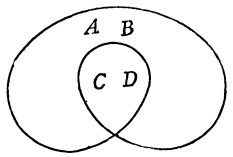
\includegraphics{scroll.png}
  \caption{Peirce's \kl{scroll}}
  \labfig{scroll}
\end{marginfigure}

\begin{quote}
  Accordingly, since logic has primarily in view argument, and since the
conclusiveness of an argument can never be weakened by adding to the premisses
or by subtracting from the conclusion, I thought I ought to take the general
form of argument as the basal form of composition of signs in my
diagrammatization; and this necessarily took the form of a ``scroll'', that is
[...] a curved line without contrary flexure and returning into itself after
once crossing itself, and thus forming an outer and an inner ``close''.
\end{quote}

\reffig{scroll} shows Peirce's drawing of the \kl{scroll} as it appears in
\cite[Fig.~5]{peirce_prolegomena_1906}. He defines its intended meaning like so
\cite[p.~534--535]{peirce_prolegomena_1906}:

\begin{quote}
  I shall call the outer boundary the Wall; and the inner, the Fence. In the
outer I scribed the Antecedent, in the inner the Consequent, of a Conditional
Proposition de inesse. [...][Thus the meaning of \reffig{scroll} is] that if
both A and B are true, then both C and D are true. [...] a Conditional de inesse
(unlike other conditionals) only asserts that either the antecedent is false or
the consequent is true. 
\end{quote}

This shows the \kl{classical} view of Peirce on \kl{EGs}, who interprets the
\kl{scroll} as signifying the \textit{conditional de inesse} --- also called
nowadays \emph{material implication}, and defined here in its disjunctive form,
expressed \kl{symbolically} by $A \limp B \defeq \neg A \lor B$. This is no
coincidence that Peirce based his most fundamental \kl{icon} on implication:
according to Lewis \sidecite[][p.~79]{Lewis1920-LEWASO-4}, he was the one who
introduced the ``illative relation'' of implication into \kl{symbolic} logic in
the first place, by giving it a distinguished \kl{symbol}, and studying
extensively the algebraic laws that govern it (including Peirce's law).

\begin{marginfigure}
  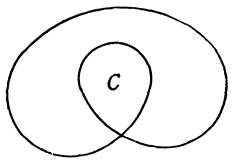
\includegraphics{empty-antecedant.png}
  \caption{Peirce's \kl{scroll} with a blank antecedant}
  \labfig{empty-antecedant}
\end{marginfigure}

\begin{marginfigure}
  $$
  \!\!\!\!\!\!\!\!\stkfig{1}{scroll-empty-antecedant}
  \!\!\!\!\xinvstep{\intro{BA}}~~~~
  G
  $$
  \caption{The rule of \kl{Blank~Antecedant}}
  \labfig{rule-empty-antecedant}
\end{marginfigure}

\subsection{Seeds of intuitionism}

\paragraph{Blank Antecedant}

A first principle that Peirce derives from the \kl{scroll} is the following
\cite[p.~534]{peirce_prolegomena_1906}:

\begin{quote}
  [...] any insertion [is] permitted in the outer close, and any omission from
the inner close. By applying the former clause of this rule to
[\reffig{empty-antecedant}], we see that this \kl{scroll} with the outer close void,
justifies the assertion that if no matter what be true, C is in any case true;
so that the two walls of the \kl{scroll}, when nothing is between them, fall
together, collapse, disappear, and leave only the contents of the inner close
standing, asserted, in the open field.
\end{quote}

\begin{marginfigure}
  ~~~\stkfig{0.8}{scroll-curried}
  \caption{Currying as \kl{scroll} nesting}
  \labfig{scroll-curried}
\end{marginfigure}

\begin{marginfigure}
  \setlength{\fboxsep}{2pt}
\setlength{\arraycolsep}{0pt}
\newcommand{\vsp}{\vspace{-0.5em}}
\newcommand{\stkf}{\tikzfig{0.9}{0.5}}
$$
\begin{array}{r@{\quad}c@{\vsp}}
                                  &\stkf{eg-currying-3} \\
       \xstep{\kl{BA}} &\stkf{eg-uncurrying-1} \\
       \xstep{\kl{Ins}} &\stkf{eg-uncurrying-2} \\
       \xstep{\kl{Deit}} &\stkf{eg-currying-0}
\end{array}
$$
  \caption{\kl{Intuitionistic} proof of currying}
  \labfig{eg-currying}
\end{marginfigure}

\begin{marginfigure}
  \setlength{\fboxsep}{2pt}
\setlength{\arraycolsep}{0pt}
\newcommand{\vsp}{\vspace{-0.5em}}
\newcommand{\stkf}{\tikzfig{0.9}{0.5}}
$$
\begin{array}{r@{\quad}c@{\vsp}}
                                  &\stkf{eg-currying-0} \\
       \xstep{\mathsf{Ins}} &\stkf{eg-currying-1} \\
       \xstep{\mathsf{Deit}} &\stkf{eg-currying-2} \\
       \xstep{\mathsf{BA}} &\stkf{eg-currying-3}
\end{array}
$$

  \caption{\kl{Intuitionistic} proof of uncurrying}
  \labfig{eg-uncurrying}
\end{marginfigure}

This first form of ``collapsing of walls'' is called the rule of \intro{Blank~Antecedant} in \cite{minghui_graphical_2019}, and corresponds \kl{symbolically} to
the equivalence $\top \limp A \semequiv{} A$. The reader might be tempted to see
the ``former clause'' that permits any insertion in the outer close as a special
case of the \kl{Insertion} principle of \kl{Alpha} (\refsec{alpha}). However, we
stress again that Peirce first identified this clause as a feature of the
\kl{scroll}, seen as the \kl{diagrammatic} embodiment of the ``general form of argument''
mentioned in a previous excerpt. The principle of \kl{Insertion} only followed as a
subsequent generalization, stemming from the analysis of the \kl{scroll} into two
nested \kl(eg){cuts} \cite[p.~535]{peirce_prolegomena_1906}:

\begin{quote}
  [...] and you will further see that a scroll is really nothing but one oval
within another.
\end{quote}

To emphasize this point, we will from now on depict \kl{scrolls} as two nested \kl(eg){cuts}
joined at a single point highlighted in orange, as illustrated in
\reffig{rule-empty-antecedant}.

\begin{remark}
  It is interesting to note that the rule of \kl{Blank~Antecedant} is not seen as
  primitive by Peirce, but as a consequence of a \emph{dynamic potential} of the
  \kl{scroll}: namely, the ability to insert anything in the outer close, at will.
  This is another manifestation of Peirce's concern for the question of
  \emph{\kl{illative atomicity}}, and is to be related to the elimination of the
  \kl{Double{-}cut} rule discussed in \refsec{atomicity}.
\end{remark}

\paragraph{Currying}

Peirce was aware of the phenomenon of \emph{currying}, expressed \kl{symbolically} by
the equivalence $A \limp B \limp C \semequiv{} A \land B \limp C$, as witnessed by
the following passage \cite[p.~535]{peirce_prolegomena_1906}:
\begin{quote}
Now, Reader, if you will just take pencil and paper and scribe the scroll
expressing that if $A$ be true, then it is true that if $B$ be true $C$ and $D$
are true [\reffig{scroll-curried}], and compare this with [\reffig{scroll}],
which amounts to the same thing in meaning, you will see that scroll walls with
a void between them collapse even when they belong to different scrolls.
\end{quote}
It is remarkable that he comes to this conclusion by a topological argument,
noting that this second form of ``collapsing of walls'', now involving two
different \kl{scrolls}, follows from the \kl{scroll} beeing composed of two nested
\kl(eg){cuts}. If we reject this interpretation by requiring that the Fence (the
inner oval) stays glued to the Wall (the outer oval), then one cannot derive
currying through the rule of \kl{Double{-}cut}, precisely because the system
only permits to collapse a Wall and a Fence continuously joined in the same
\kl{scroll}, by the weaker rule of \kl{Blank~Antecedant}. Fear not however, as one can
still derive the currying and uncurrying laws in this \kl{intuitionistic} setting,
but through the additional use of the insertion and deiteration rules, as
depicted in \reffig{eg-currying} and \reffig{eg-uncurrying}. Yet we find that
Peirce's insight on the topological explanation of currying in the \kl{classical}
setting remains noteworthy.

\begin{remark}
Note that in \reffig{eg-currying} and \reffig{eg-uncurrying}, we give
\emph{\kl{forward}} proofs that rewrite the premiss of the argument into its
conclusion, rather than \emph{\kl{backward}} proofs that rewrite a \kl{goal}
into the empty $\SA$, as we usually did in previous chapters. \kl{Forward}
proofs correspond to Peirce's usage of the \kl{illative transformations} --- and
thus to what can be found in most of the literature on \kl{EGs}, and have the
advantage of being more economical in space by leaving the \kl{goal} implicit.
One can easily go from a \kl{forward} proof to a \kl{backward} one as shown by
the \emph{deduction theorem} of Sowa \cite[Section 6]{sowa_peirces_2011}, which
also applies in the \kl{intuitionistic} setting by substituting the rule of
\kl{Double{-}cut} with the rule of \kl{Blank~Antecedant}.
\end{remark}

\subsection{Parallel conclusions}

\paragraph{The $n$-ary scroll}

In \cite{oostra_graficos_2010}, A. Oostra proposes to take the above remark
seriously, by reifying the \kl{scroll} as a primitive \kl{icon} of \kl{EGs}
(``\emph{rizo}'' in Spanish), that exists alongside the \kl(eg){cut}
(``\emph{corte}''), and is distinguished from it. In fact he goes further than
this, and proposes to generalize both the \kl(eg){cut} and the \kl{scroll} into
an $n$-ary construction called the \intro{curl} (``\emph{bucle}''), where $n$ is
the number of inner closes, called \emph{loops} (``\emph{lazos}'').
\reffig{five-loops} shows an example of \kl{curl} with five loops. In
\cite{minghui_graphical_2019}, the \kl{curl} is simply called \intro{$n$-ary
scroll}, and is analyzed into the outer area (that enclosed by the Wall) called
the \intro{outloop}, and the inner areas (those enclosed by the $n$ Fences, i.e.
the loops of Oostra) called the \intro{inloops}. Then \kl(eg){cuts} and
\kl{scrolls} are indeed special cases of \kl{$n$-ary scrolls}, respectively with
$n = 0$ and $n = 1$.

\begin{marginfigure}
  \stkfig{1}{five-loops}
  \caption{A \kl{curl} with five loops}
  \labfig{five-loops}
\end{marginfigure}

Like the unary \kl{scroll}, the \kl{$n$-ary scroll} is to be read as an
implication whose antecedant is the content of the \kl{outloop}, and consequent the
content of the \kl{inloops}. The generalization then consists in taking the
\emph{disjunction} of the contents of all \kl{inloops}: this reflects nicely the
etymological meaning of the word ``disjunction'', since the \kl{inloops} enclose
\emph{disjoint} areas of the \kl{outloop} to which they are attached. Then the
\kl[$n$-ary scroll]{$5$-ary scroll} of \reffig{five-loops} is read as the
formula $a \limp b \lor c \lor d \lor e \lor f$; and the \kl[$n$-ary
scroll]{$0$-ary scroll} obtained by removing all \kl{inloops} from the latter as $a
\limp \bot$, since a $0$-ary disjunction is naturally evaluated to its neutral
element $\bot$. This coincides with the \kl{intuitionistic} reading of negation
$\neg A \defeq A \limp \bot$, and is thus consistent with the interpretation of
\kl(eg){cuts} as negations.

\paragraph{Continuity}

\begin{marginfigure}
  $$
\begin{array}{c}
  \begin{array}{cc}
    \stkfig{1}{scroll-disj} & A \lor B \\
    \stkfig{1}{scroll-imp} & A \limp B \\[1em]
    \multicolumn{2}{c}{\not=} \\
    \stkfig{1}{eg-disj} & \neg (\neg A \land \neg B) \\
    \stkfig{1}{eg-imp} & \neg (A \land \neg B)
  \end{array}
\end{array}
$$
  \caption{Continuity, disjunction and implication in \kl{IEGs}}
  \labfig{eg-disj-imp}
\end{marginfigure}

With this interpretation of the \kl{$n$-ary scroll}, the \kl{Alpha} encodings of
disjunction and implication as nested \kl(eg){cuts} are no longer valid, because
they are not \kl{intuitionistically} equivalent to the associated binary and
unary \kl[$n$-ary scroll]{scrolls}. This is illustrated in \reffig{eg-disj-imp},
where the closeness in meaning is reflected \kl{iconically} (but not
\kl{symbolically}) in the fact that the graphs only differ in the
\emph{continuity} (or lack thereof) between \kl{inloops} and their \kl{outloop}. Indeed,
contrary to nested \kl(eg){cuts}, any \kl{$n$-ary scroll} can be drawn by a
\emph{continuous} movement of the pen, producing a self-intersecting curve as
described by Peirce in \cite{peirce_prolegomena_1906}.

This might be related to other manifestations of the notion of continuity in the
semantics of \kl{intuitionistic} logic, such as the well-known Stone-Tarski
interpretation of formulas as topological spaces \cite{stone_topological_1938},
and the interpretation of proofs as continuous maps in the \emph{denotational
semantics} of Dana Scott \sidecite{10.5555/218742.218744}. Before the advent of
Oostra's \kl{IEGs}, Zalamea gave a detailed analysis of Peirce's philosophy of
the \emph{continuum}, how it relates to modern developments in mathematics, and
how it is embodied in \kl{existential graphs} \cite{zalamea_peirces_2003}.
Actually according to Oostra \sidecite[][p.~162]{oostra_advances_2022}, ``the
possibility of developing \kl{intuitionistic} existential graphs was first
suggested by Zalamea in the 1990s \cite{zalamea_ieg_1,zalamea_ieg_2}''.

\subsection{Quantifiers}

More generally, a \kl{$n$-ary scroll} with atoms $G \deq a_1, \ldots, a_m$ in its
\kl{outloop} and $\Delta \deq \begin{pmatrix} a_{1,1} & \ldots & a_{1,p_1} \\
  \vdots & \ddots & \vdots \\
  a_{n,1} & \ldots & a_{1,p_n}
\end{pmatrix}$
in its \kl{inloops}, where each row $H_j$ in $\Delta$ encodes an \kl{inloop}, can be
interpreted as the formula
$$\bigwedge_{i = 1}^{m}{a_i} \limp \bigvee_{j = 1}^{n}\bigwedge_{k = 1}^{p_n}{a_{j,k}}$$
\begin{marginfigure}
  $$
  \!\!\!\!
  \!\!\!\!
  \!\!\!\!
  \begin{array}{c}
    \tikzfig{0.85}{0.85}{curl-geom} \vspace{1.5em}\\
    \forall \bx. \left(\bigwedge G \limp \bigvee_{j = 1}^{n}\exists \bx_j. \bigwedge H_j\right)
  \end{array}
  $$
  \caption{Formula interpretation of the \kl{$n$-ary scroll}}
  \labfig{curl-geom}
\end{marginfigure}
If one adds \emph{\kl(eg){binders}} to the mix (see \refsec{gardens}) by having $\gamma \deq
\garden{\bx}{G}$ as \kl{outloop}, and
$\Xi \deq \begin{pmatrix}
  \bx_1 \\
  \vdots \\
  \bx_n
\end{pmatrix} \cdot \Delta$ as \kl{inloops}, then the interpretation is extended into
the formula
$$\forall \bx. \left(\bigwedge_{i = 1}^{m}{a_i} \limp \bigvee_{j = 1}^{n}\exists \bx_j. \bigwedge_{k = 1}^{p_n}{a_{j,k}}\right)$$
as depicted in \reffig{curl-geom}. Typically, the particular case where $\gamma
\deq \garden{x}{\emptyset}$ and $\Xi \deq (\emptyset) \cdot (p(x))$ encodes the graph
$$\stkfig{1}{scroll-forall}$$
expressing the universal quantification $\forall x. p(x)$, and the case where
$\gamma \deq \garden{\emptyset}{\emptyset}$ and $\Xi \deq (x) \cdot (p(x))$ the graph
$$\stkfig{1}{scroll-exists}$$
expressing the existential quantification $\exists x. p(x)$. The interpretation
is invariant under \kl(eg){polarity}, meaning that for instance the graphs
$$\stkfig{1}{scroll-neg-forall} \text{   and   } \stkfig{1}{scroll-neg-exists}$$
obtained by enclosing the previous graphs in a \kl(eg){cut} are interpreted with the
same quantifiers, as the formulas $\neg \forall x. p(x)$ and $\neg \exists x.
p(x)$. In \kl{Beta}, we would have exploited the \kl{classical} equivalences
$\neg \forall x. A \semequiv{} \exists x. \neg A$ and $\neg \exists x. A \semequiv{}
\forall x. \neg A$ (justified by the \kl{Double{-}cut} principle) in order to
interpret them as $\exists x. \neg p(x)$ and $\forall x. \neg p(x)$, emphasizing
the idea that \kl(eg){positive} and \kl(eg){negative} \kl(eg){binders} encode
respectively $\exists$ and $\forall$. But this is not possible anymore with the
\kl{intuitionistic} interpretation of \kl{$n$-ary scrolls}, where the
$\exists/\forall$ duality is replaced by the \kl{inloop}/\kl{outloop} distinction. In
fact, we are tempted to further qualify this distinction of \emph{adjunction},
following a classical result of Lawvere in the context of categorical logic
\sidecite{lawvere_quantifiers_sheaves}.

\subsection{Coherent formulas}

Lawvere is also known for some contributions to the study of \intro{geometric
logic} \sidecite{lawvere_geometric}, a subset of the formulas of \kl{FOL} first
discovered by Skolem \sidecite{skolem_geometric} that is capable of expressing
many mathematical theories, and has close connections to \emph{topos theory}.
Quite remarkably, the interpretation of \kl{$n$-ary scrolls} coincides exactly
with the class of \intro{coherent formulas}, which are the formulas of
\kl{geometric logic} where infinitary disjunctions are restricted to finitary
ones. There is a difference however: the full syntax of \kl{IEGs} allows for
arbitrary \emph{nestings} of \kl{$n$-ary scrolls} inside eachother, i.e. the
multisets $G$ and $H_j$ in \reffig{curl-geom} can contain \kl{$n$-ary scrolls}
in addition to atoms; while \kl{coherent formulas} are restricted to atoms.

\kl{Coherent formulas} have some nice properties, which might also apply to \kl{IEGs} to
some extent. We only mention two important ones:
\begin{description}
  \item[Completeness] Every \kl{first-order} \kl{theory} has a coherent conservative
  extension, making \kl{coherent formulas} (and thus non-nested \kl{$n$-ary scrolls}) in
  principle as expressive as arbitrary \kl{first-order} formulas
  \sidecite{negri_geometric}.
  
  \item[Automation] \kl{Coherent formulas} benefit from faster proof-search
  procedures compared to arbitrary formulas, making automation more tractable
  computationally. They also allow the direct encoding of many reasoning
  problems, thanks to their use of the full set of connectives and quantifiers
  of \kl{FOL}; and avoiding complex encodings (as can be found e.g. in SMT
  solvers) is crucial in \emph{interactive} theorem proving, where the user and
  the computer manipulate the same formulas in \kl{goal}s
  \sidecite{bezem_automating_2005}. This has been exploited already in some
  domain-specific theorem provers, like the \intro{Larus} prover that
  automatically generates illustrated proofs in geometry\sidenote{Incidentally,
  projective geometry was one of the motivating applications that led Skolem to
  identify the class of \kl{coherent formulas} \cite{bezem_automating_2005}.}
  \sidecite{narboux_larus}.
  
  \begin{remark}
  Thus with \kl{IEGs}, one becomes able to reason \emph{geometrically} on geometric
  formulas that speak about geometry: another beautiful incarnation of the
  reflexivity at work in Peirce's \kl{iconic} logic.
  \end{remark}
\end{description}

\section{Flowers}\labsec{Flowers}

\subsection{Blooming}

As we have seen, the ($n$-ary) \kl[$n$-ary scroll]{scroll} is a powerful
\kl{icon}, because it captures the distinction between \kl{classical} and
\kl{intuitionistic} logic as being a matter of \emph{continuity} between the
space of inputs/hypotheses (\kl{outloop}) and the spaces of outputs/conclusions
(\kl{inloops}), reflecting an intuition discovered much later in the denotational
semantics of the \kl{$\lambda$-calculus}. However as a \kl{diagrammatic}
component to be operated upon through \kl{direct manipulation}, it has one
notable flaw, also shared with the \kl{classical} \kl(eg){cut}-based syntax: it
quickly induces heavy nestings of curves in the plane, making even a simple
graph like that of \reffig{scroll-curried} hard to read for an untrained eye.

\begin{marginfigure}
  $$
  \tikzfig{1}{0.4}{scroll-inside-out}
  $$
  \caption{Turning a \kl[$n$-ary scroll]{$5$-ary scroll} inside-out}
  \labfig{scroll-inside-out}
\end{marginfigure}

Before devising an alternative syntax, one should ask: what are the essential
features of the \kl[$n$-ary scroll]{scroll} that we want to preserve? Following
the previous observations, we identified two of them:
\begin{description}
  \item[Continuity] the \kl[$n$-ary scroll]{scroll is} a self-intersecting
  continuous curve, which can be drawn in one stroke of the pen;
  \item[Polarity] this curve delineates two kinds of areas: \kl{inloops} that have
  the same \kl(eg){polarity} as the area on which the \kl[$n$-ary
  scroll]{scroll} is scribed, and the \kl{outloop} which has the opposite
  \kl(eg){polarity}.
\end{description}

Fortunately, these two properties are preserved when turning \kl{inloops}
\emph{inside-out}, as illustrated in \reffig{scroll-inside-out}. This might be
because the very process of turning inside-out can be seen as a continuous
movement in three-dimensional space, where the \kl{inloops} are rotated around their
intersection points with the \kl{outloop}. In this way, we have effectively divided
the amount of curve-nesting in \kl[$n$-ary scroll]{scrolls} by two. And as an
added bonus, the new \kl{icon} is reminiscent of a \emph{flower}, as if it had
bloomed from its curled bud; or as if the pistol cylinder from
\reffig{five-loops} had transformed into a \emph{pistil}, and its bullet
chambers into \emph{petals}\sidenote{As the saying goes: make love, not war.}.

\begin{marginfigure}
  $$
  \!\!\!\!
  \!\!\!\!
  \!\!\!\!
  \!\!\!\!
  \stkfig{0.65}{flowers}
  $$
  \vspace{-3em}
  \caption{Nested flowers}
  \labfig{flowers}
\end{marginfigure}

From that point onwards, we decided to fully embrace the flower \kl{metaphor}:
first in our drawing style as witnessed in \reffig{flowers}, but also in our
syntactic terminology, to be introduced in the next pages. \kl(eg){Negative}
\kl{outloops} are now drawn as \emph{yellow} pistils for a more colorful experience,
and \kl{inloops} as transparent petals, i.e. of the same color as the area on which
they are scribed. We also drop the requirement that petals should intersect
their pistil at a single point, for purely aesthetic reasons.

\subsection{Multisets}

As we did for \kl{classical} \kl{EGs} in \refsec{multisets} and \refsec{gardens}, we are
now going to distill the syntactic essence of flowers into an inductive,
(multi)set-based data structure. This will allow for a more compact textual
notation, that is better suited to \kl{proof-theoretical} study.

In \refsec{beta}, we explained how the graphs of \kl{Beta} allow to represent
purely relational statements, without function symbols. Since functions are just
deterministic relations, one can in principle formalize any \kl{first-order}
\kl{theory} in this syntax\sidenote{Conversely, every relation can be faithfully
encoded as its characteristic function, which is the basis for the formalization
of mathematics in \emph{\kl{type theories}}.}. However it is much more
convenient to have a dedicated syntax for functions, and we will thus introduce
them as is usually done in predicate calculus.

\begin{definition}[First-order signature]
  A \intro{first-order signature} is a triplet $\mathcal{\Sigma} = (
  \intro*\fsymbs, \intro*\psymbs, \intro*\arity )$, where $\fsymbs$ and $\psymbs$ are
  respectively the countable sets of \emph{function} and \emph{predicate}
  symbols of $\Sigma$, and $\arity : \fsymbs \cup \psymbs \to \nats$ gives an
  \emph{arity} to each symbol.
\end{definition}

\AP
In the following, we assume given a denumerable set of variables $\intro*\vars$
and a \kl{first-order signature} $\Sigma$.

\begin{definition}[Terms]
  The set of terms $\intro*\terms$ is defined inductively as follows:
  \begin{description}
    \item[(Variable)] If $x \in \vars$ then $x \in \terms$;
    \item[(Application)] If $f \in \fsymbs$ and $\tvec{t}
    \in \terms^{\arity(f)}$, then $f(\tvec{t}) \in \terms$.
  \end{description}
\end{definition}

\begin{digression}
  According to the Merriam-Webster dictionary \cite{corolla}, the word
  ``corollary'' has \emph{botanical} etymological roots:
  \begin{quote}
    [...] the seed of corollary was planted initially by the Latin noun corōlla
    meaning ``small wreath of flowers'', which later bloomed into another Latin
    noun, corōllārium, referring to a garland given as a reward as well as to a
    gratuity or an unsolicited payment. [...] The formality of corollary is
    thanks to its formal roots [...]
  \end{quote}
  Then our flower metaphor is a meaningful tribute to these origins: the
  \kl{petals} (\kl{corolla}) of a flower can literally be seen as the
  \emph{corollaries} of its \kl{pistil}, when the latter happens to be true.
\end{digression}

\begin{definition}[Flowers]\labdef{flowers}
  The sets of \emph{flowers} $\intro*\flowers$ and \emph{gardens}
  $\intro*\gardens$ are defined mutually inductively as follows:
  \begin{description}
    \itemAP[(Atom)] If $p \in \psymbs$ and $\tvec{t} \in
    \terms^{\arity(p)}$, then $p(\tvec{t}) \in \flowers$;
    \itemAP[(Garden)] If $\bx \subset \vars$ is a finite set and $\Phi
    \subset \flowers$ a finite multiset, then $\intro*\garden{\bx}{\Phi} \in
    \gardens$;
    \itemAP[(Flower)] If $\gamma \in \gardens$ and $\Delta \subset \gardens$
    is a finite multiset, then $\intro*\flower{\gamma}{\Delta} \in \flowers$.
  \end{description}
\end{definition}

Any finite set $\bx \subset \vars$ of variables is called a \intro{sprinkler},
finite multiset $\Phi \subset \flowers$ of flowers a \intro{bouquet}, and finite
multiset $\Gamma \subset \gardens$ of gardens a \intro{corolla}. We will often
write gardens as $\garden{x_1, \ldots, x_n}{\phi_1, \ldots, \phi_m}$, where the
$x_i$ are called \intro{binders}; and non-atomic flowers as
$\flower{\gamma}{\delta_1 \sep \ldots \sep \delta_n}$, where $\gamma$ is the
\intro{pistil}, and the $\delta_i$ are called \intro{petals}. We write
$\intro*\fset{i}{n}{E_i}$ to denote a finite (multi)set of size $n$ with
elements $E_i$ indexed by $1 \leq i \leq n$. We also omit writing the empty
(multi)set, accounting for it with blank space as is done in \kl{sequent}
notation or in \kl{EGs}; in particular, $\garden{{}}{{}}$ stands for the empty
garden $\garden{\emptyset}{\emptyset}$, $\flower{\gamma}{{}}$ for the flower
with no \kl{petals} $\flower{\gamma}{\emptyset}$, and
$\flower{\gamma}{\garden{{}}{{}}}$ for the flower with one empty \kl{petal}.

Note that the order of precedence of operators is
$\mathop{,} < \garden{{}}{{}} < \mathop{;} < \mathop{\flower{}{}}$
so that for instance, the string
$$\flower{\garden{x_1, x_2}{\phi_1, \phi_2}}{\garden{y_1}{\psi, (\flower{\gamma}{\Delta})} \sep \garden{y_2}{\Phi}}$$
is parsed as the flower
% $$\left(\flower{\left(\garden{\{x_1, x_2\}}{\{\phi_1,
% \phi_2\}}\right)}{\{\left(\garden{\{y_1\}}{\{\psi,
% \left(\flower{\gamma}{\Delta}\right)\}}\right) \sep
% \left(\garden{\{y_2\}}{\Phi}\right)\}}\right)$$ where constructed finite
% (multi)sets are delimited with $\{\}$, and constructed flowers/gardens are
% delimited with $()$.
\vspace{-6em}
$$\stkfig{1}{parsed-flower}$$
\vspace{-6em}

\begin{margintable}
  \centering
  \begin{tabular}{|c|c|}
    \hline
    \bfseries Kind & \bfseries Letters \\
    \hline
    Variables ($\vars$) & $x, y, z$ \\
    Terms ($\terms$) & $t, u, v$ \\
    Flowers ($\flowers$) & $\phi, \psi, \xi$ \\
    Gardens ($\gardens$) & $\gamma, \delta$ \\
    \kl{Sprinklers} & $\bx, \by, \bz$ \\
    Term vectors & $\tvec{t}, \tvec{u}, \tvec{v}$ \\
    \kl{Substitutions} & $\sigma, \tau$ \\
    \kl{Bouquets} & $\Phi, \Psi, \Xi$ \\
    \kl{Corollas} & $\Gamma, \Delta$ \\
    \kl{Contexts} & $\Phi\hole, \Psi\hole, \Xi\hole$ \\
    \kl{Theories} & $\mathcall{T}, \mathcall{U}$ \\
    \hline
  \end{tabular}
  \caption{Notational conventions for meta-variables}
  \labtab{letters}
\end{margintable}

Also to improve readability, we will most of the time omit the garden dot
`$\cdot$' when the \kl{sprinkler} is empty, writing $\Phi$ instead of
$\garden{{}}{\Phi}$.

\begin{remark}
  In some places the choice of letter for meta-variables will be important to
  disambiguate the kind of syntactic object we denote. \reftab{letters}
  summarizes our chosen notational conventions in this respect.
\end{remark}

As usual, we introduce a \emph{\kl{depth}} measure that will allow us to reason
inductively on the structure of flowers:
\begin{definition}[Depth]
  The \reintro{depth} $\intro*\sdepth{-}$ of a flower or garden is defined mutually
  recursively as follows:
  \begin{align*}
    \sdepth{p(\tvec{t})} &= 0 \\
    \sdepth{\garden{\bx}{\Phi}} &= \max_{\phi \in \Phi}{\sdepth{\phi}} \\
    \sdepth{\flower{\gamma}{\Delta}} &= 1 + \max(\sdepth{\gamma}, \max_{\delta \in \Delta}{\sdepth{\delta}})
  \end{align*}
\end{definition}

\subsection{Substitutions}

We now proceed with routine definitions for handling variables and \kl{substitutions}
of terms in flowers.

\begin{definition}[Free variables]\labdef{fv}
  
  The sets of \intro{free variables} $\intro*\fv(-)$ of a term, flower,
  \kl{bouquet} or garden are defined mutually recursively as follows:
  \begin{align*}
    \fv(x) &= \{x\} &
    \fv(\Phi) &= \bigcup_{\phi \in \Phi}{\fv(\phi)} \\
    \fv(f(\tvec{t})) &= \bigcup_{t \in \tvec{t}}{\fv(t)} &
    \fv(\garden{\bx}{\Phi}) &= \fv(\Phi) \setminus \bx \\
    \fv(p(\tvec{t})) &= \bigcup_{t \in \tvec{t}}{\fv(t)} &
    \fv(\flower{\garden{\bx}{\Phi}}{\Delta}) &= \fv(\garden{\bx}{\Phi}) \cup \bigcup_{\garden{\by}{\Psi} \in \Delta}{\fv(\garden{\bx, \by}{\Psi})}
  \end{align*}
  We say that a term, flower, \kl{bouquet} or garden is \emph{closed} when its set of
  \kl{free variables} is empty.
  % The sets of closed terms, flowers and gardens are denoted respectively by
  % $\closed{\terms}$, $\closed{\flowers}$ and $\closed{\gardens}$.
\end{definition}

\begin{remark}\labremark{flower-scope}
Note that the scope of a \kl{binder} located in a \kl{pistil} extends both to the \kl{pistil}
\emph{and} to all its attached \kl{petals}, whereas for a \kl{binder} located in a \kl{petal}
it is limited to said \kl{petal}. This is reflected in the above definition of \kl{free
variables} for (non-atomic) flowers, and is visually explained by the nesting of
curves in an \kl{$n$-ary scroll}.
\end{remark}

\begin{definition}[Bound variables]
  % The set of \emph{bound variables} $\bv(\Phi\hole)$ of a context $\Phi\hole$ is defined
  % inductively as follows:
  % \begin{align*}
  %   \bv(\Psi, \hole) &= \emptyset \\
  %   \bv(\Psi, (\flower{\garden{\bx}{X}}{\Delta})) &= \bx \cup \bv(X) \\
  %   \bv(\Psi, (\flower{\garden{\bx}{\Phi}}{\garden{\by}{X} \sep \Delta})) &= \bx \cup \by \cup \bv(X)
  % \end{align*}
  The sets of \intro{bound variables} $\intro*\bv(-)$ of a flower, \kl{bouquet}
  or garden are defined mutually recursively as follows:
  \begin{align*}
    \bv(p(\tvec{t})) &= \emptyset &
    \bv(\garden{\bx}{\Phi}) &= \bx \cup \bv(\Phi) \\
    \bv(\Phi) &= \bigcup_{\phi \in \Phi}{\bv(\phi)} &
    \bv(\flower{\gamma}{\Delta}) &= \bv(\gamma) \cup \bigcup_{\delta \in \Delta}{\bv(\delta)}
  \end{align*}
\end{definition}

To avoid reasoning about $\alpha$-equivalence, we adopt in this work the
so-called \emph{Barendregt convention} that all variable \kl{binders} are distinct,
both among themselves and from eventual \kl{free variables}. Formally, we assume that
for any \kl{bouquet} $\Phi$, the two following conditions hold:
\begin{enumerate}
  \item computing $\bv(\Phi)$ as a multiset gives the same result as computing
  it as a set;
  \item $\bv(\Phi) \cap \fv(\Phi) = \emptyset$.
\end{enumerate} 
% To preserve this convention, in this paper we will only consider
% \emph{non-circular} substitutions $\sigma$ where $x \not\in \fv(\sigma(x))$ for
% all $x \in \dom(\sigma)$.

To define \kl{substitutions}, we introduce a general notion of \emph{function
\kl{update}}, which will be useful for the semantic evaluation of flowers in
\refsec{Semantics}.

\begin{definition}[Function update]\labdef{update}
  Let $A, B$ be two sets, $f, g : A \to B$ two functions and $R \subseteq A$
  some subset of their domain. The \intro{update} of $f$ on $R$ with $g$ is the
  function defined by:
  $$
  (f \intro*\upd{R} g)(x) =
  \begin{cases}
    g(x) &\text{if $x \in R$} \\
    f(x) &\text{otherwise}
  \end{cases}
  $$
  $\update{-}{-}{-}$ is left-associative, that is
  $\update{f}{R}{\update{g}{S}{h}} = \update{(\update{f}{R}{g})}{S}{h}$. Also if
  $f$ or $g$ is the identity function $\intro*\idsubst$ we omit writing it, i.e.
  $\update{f}{R}{{}} = \update{f}{R}{\idsubst}$ and $\update{{}}{R}{g} =
  \update{\idsubst}{R}{g}$.
\end{definition}

\begin{definition}[Substitution]
  A \intro{substitution} is a function $\sigma : \vars \to \terms$ with a finite
  \intro{support} $\dom(\sigma) = \compr{x}{\sigma(x) \not= x}$. By abuse of
  notation, we will write $\sigma : \bx \to \terms$ to denote a \kl{substitution}
  $\sigma$ whose \kl{support} is $\bx$. The domain of \kl{substitutions} is extended to
  terms, flowers, \kl{bouquets} and gardens mutually recursively as follows:
  \begin{align*}
    \sigma(f(t_1, \ldots, t_n)) &= f(\sigma(t_1), \ldots, \sigma(t_n)) \\
    \sigma(p(t_1, \ldots, t_n)) &= p(\sigma(t_1), \ldots, \sigma(t_n)) \\
    \sigma(\phi_1, \ldots, \phi_n) &= \sigma(\phi_1), \ldots, \sigma(\phi_n) \\
    \sigma(\garden{\mathbf{x}}{\Phi}) &=
      \garden{\mathbf{x}}{\restr{\sigma}{\mathbf{x}}(\Phi)} \\
    \sigma(\flower{\garden{\mathbf{x}}{\Phi}}{\delta_1 \sep \ldots \sep \delta_n}) &=
      \flower{\sigma(\garden{\mathbf{x}}{\Phi})}{\restr{\sigma}{\mathbf{x}}(\delta_1) \sep \ldots \sep \restr{\sigma}{\mathbf{x}}(\delta_n)}
  \end{align*}

\end{definition}

\begin{definition}[Capture-avoiding substitution]
  We say that a \kl{substitution} $\sigma : \bx \to \terms$ is
  \intro{capture-avoiding} in a \kl{bouquet} $\Phi$ if $\fv(\sigma(x)) \cap \bv(\Phi)
  = \emptyset$ for every $x \in \bx$.
  % $\fv(\sigma(x)) \cap \bv(\phi) = \emptyset$ for every $x \in
  % \bx$, or $\bx \cap \fv(\phi) = \emptyset$.
  % \begin{itemize}
  %   \item $\phi = p(\tvec{t})$;
  %   \item $\phi =
  %   \flower{\garden{\by}{\Phi}}{\fset{i}{n}{\garden{\bz_i}{\Psi_i}}}$,
  %   $\fv(\sigma(x)) \cap \left(\by \cup \bigcup_{i = 1}^{n}{\bz_i}\right) =
  %   \emptyset$ for every $x \in \bx \cap \left(\fv(\Phi) \cup \bigcup_{i =
  %   1}^{n}{\fv(\Psi_i)}\right)$, and $\sigma$ is capture-avoiding in $\Phi \cup
  %   \bigcup_{i = 1}^{n}{\Psi_i}$.
  %   % \item $\bx \cap \fv(\phi) = \emptyset$.
  % \end{itemize}
\end{definition}

\section{Calculus}\labsec{Calculus}

\subsection{Preliminary definitions}

\paragraph{Contexts}

Equipped with an inductive syntax, we can now express formally the \kl{inference
rules} of our \kl{flower calculus}, just as we did for \kl{Alpha}
(\refsec{multisets}) and \kl{Beta} (\refsec{gardens}). There, graphs and their
\kl{contexts} were defined as multisets of \kl(beta){nodes}, which have now turned
into \kl{bouquets} of flowers:

\begin{definition}[Context]
  A \intro{context} $\Phi\hole$ is a \kl{bouquet} which contains exactly one
  occurrence of a special flower written $\hole$, called its \reintro{hole}. The
  \kl{hole} can always be \emph{filled} (substituted) with any other
  \kl{bouquet} $\Psi$ or \kl{context} $\Xi\hole$, producing a new \kl{bouquet}
  $\cfill{\Phi}{\Psi}$ or \kl{context} $\cfill{\Phi}{\Xi\hole}$. In particular,
  filling with the empty \kl{bouquet} will yield a \kl{bouquet}
  $\cfill{\Phi}{\phantom{\Phi}}$, which is just $\Phi\hole$ with its \kl{hole}
  removed. A \emph{flower context} $\phi\hole$ is a \kl{context} with exactly
  one flower.
\end{definition}

\begin{definition}[Depth]
  The \intro{depth} $\intro*\cdepth{\Phi\hole}$ of a \kl{context} $\Phi\hole$ is
  defined recursively as follows:
  \begin{align*}
    \cdepth{\Psi, \hole} &= 0 \\
    \cdepth{\Psi, (\flower{\garden{\bx}{\Phi\hole}}{\Delta})} &= 1 + \cdepth{\Phi\hole} \\
    \cdepth{\Psi, (\flower{\gamma}{\garden{\bx}{\Phi\hole} \sep \Delta})} &= 1 + \cdepth{\Phi\hole}
  \end{align*}
\end{definition}

Contrarily to \kl{EGs} (\refdef{eg-inv}), the number of inversions of a \kl{context} does
not coincide with its \kl{depth}, since \kl{petals} increase \kl{depth} but preserve \kl{polarity}:

\begin{definition}[Inversions]
  The number of \emph{inversions} $\intro*\inv(\Phi\hole)$ of a \kl{context} $\Phi\hole$ is
  defined recursively by:
  \begin{align*}
    \inv(\Psi, \hole) &= 0 \\
    \inv(\Psi, (\flower{\garden{\bx}{\Phi\hole}}{\Delta})) &= \inv(\Phi\hole) + 1 \\
    \inv(\Psi, (\flower{\gamma}{\garden{\bx}{\Phi\hole} \sep \Delta})) &= \inv(\Phi\hole)
  \end{align*}
\end{definition}

\begin{definition}[Polarity]
  \phantomintro{polarity}
  We say that a \kl{context} $\Phi\hole$ is \intro{positive} if
  $\inv(\Phi\hole)$ is even, and \intro{negative} otherwise. We denote \kl{positive}
  and \kl{negative} \kl{contexts} respectively by $\Phi^+\hole$ and $\Phi^-\hole$.
\end{definition}

\paragraph{Pollination}

In order to formulate the equivalent of the (de)iteration rules of \kl{EGs} for
flowers, we introduce a \emph{\kl{pollination}} relation that captures the
availability of a flower in a given \kl{context}, akin to the \emph{justification}
relation of \refsubsec{scientific-way}:

\begin{definition}[Pollination]\labdef{pollination}
  
  We say that a flower $\phi$ can be \intro{pollinated} in a \kl{context}
  $\Phi\hole$, written $\intro*\chyp{\phi}{\Phi\hole}$, when there exists a
  \kl{bouquet} $\Psi$ with $\phi \in \Psi$ and \kl{contexts} $\Xi\hole$ and
  $\Xi_{0}$ such that either:
  \begin{description}
    \itemAP[(\intro{Cross-pollination})] $\Phi\hole = \cfill{\Xi}{\Psi,
    \Xi_{0}}$;
    \itemAP[(\intro{Self-pollination})] $\Phi\hole =
    \cfill{\Xi}{\flower{\garden{\bx}{\Psi}}{\garden{\by}{\Xi_{0}}
    \sep \Delta}}$ for some $\bx, \by, \Delta$.
  \end{description}
  A \kl{bouquet} $\Psi$ can be \kl{pollinated} in $\Phi\hole$, written
  $\chyp{\Phi}{\Phi\hole}$, if $\chyp{\phi}{\Phi\hole}$ for all $\phi \in \Phi$.
\end{definition}

\begin{marginfigure}
  $$
  \!\!\!\!
  \!\!\!\!
  \!\!\!\!
  \begin{array}{c}
    \tikzfig{1}{0.5}{cross-pollination} \vspace{-2em} \\
    \text{\textit{\kl{Cross-pollination}}} \vspace{-1em} \\
    \tikzfig{1}{0.5}{self-pollination} \vspace{-2em} \\
    \text{\textit{\kl{Self-pollination}}}
  \end{array}
  $$
  \caption{\kl{Pollination} in flowers}
  \labfig{pollination}
\end{marginfigure}

We now employ the \kl{metaphor} of \emph{\kl{pollination}} to speak about
(de)iteration in flowers. This is illustrated in \reffig{pollination}, where the
blue dot marks the location of the justifying/\kl{pollinating} occurrence of
$\phi$, and the red dots all the areas that it (locally)
justifies/\kl{pollinates}, and thus where $\phi$ can be
(de)iterated\sidenote{\reffig{pollination} summarizes visually the flow of
information in flowers, just like \reffig{eg-local-justification} summarized the
flow of information in \kl{EGs}, and \reffig{bubbles-porosity} in bubbles. From
a UI point of view, all these figures can be understood as kind of
``cheatsheets'', that indicate with arrows the allowed drag-and-drop moves for
importing a statement (the source of the \kl{DnD}) into a new \kl{context} (the
destination of the \kl{DnD}).}. We distinguish two cases of
\emph{\kl{cross-pollination}} and \emph{\kl{self-pollination}}, as botanists do
when describing the reproduction of flowers. This distinction does not exist in
\kl{classical} \kl{EGs}, because \kl{pistils} and \kl{petals} are both
identified as instances of \kl(eg){cuts}\sidenote{The same phenomenon is at work
in \emph{\kl{subformula linking}} (\refch{sfl}): \kl{self-pollination} and
\kl{cross-pollination} correspond respectively to the \emph{\kl(dnd){backward}}
$\back$ and \emph{\kl(dnd){forward}} $\forw$ \kl{interaction operators}, which
are collapsed into a single interaction operator $\ast$ in the original
formulation of \kl{subformula linking} for classical linear logic
\cite{Chaudhuri2013}.}. If we were to replace \kl{binders} by \kl{LoIs}
(\kl{lines of identity}, see \refsec{beta}), then the \kl{pollination} relation would
also prescribe in which areas \kl{LoIs} can be extended/iterated, providing an
explanation for the scope of \kl{binders} (\refremark{flower-scope}).

\subsection{Rules}

As has become standard in this thesis, we define the \kl{flower calculus} as a
\emph{\kl{rewriting system}} on \kl{bouquets}, presented in \reffig{flower-calculus} as a
set of unary \kl{deep inference} rules: when read \emph{top-down}, they correspond to
usual inferences from premiss to conclusion, and will be justified by the
soundness theorem of \refsec{Soundness}.
But the more interesting direction, and the one around which the calculus has
been designed, is when you read the rules \emph{bottom-up}: then they are indeed
\kl{rewriting rules}, telling you the different ways in which you can choose to
simplify a \kl{goal}. This is how the \emph{graphical} version of the rules is
presented in \reffig{natural-graphical} and \reffig{cultural-graphical}.

Let us now describe the rules in more detail, starting with the fragment that is
a direct adaptation of the rules of \kl{Beta} (\reffig{beta}):

\begin{description}
  \item[Blank~Antecedant (\kl{epis})]
    
    \begin{marginfigure}
      $$
      \R[\intro{epis{\da}}]
        {\Phi}
        {\flower{\garden{{}}{{}}}{\garden{{}}{\Phi}}}
      $$
      \caption{Converse of \kl{epis} rule}
      \labfig{flowers-episda}
    \end{marginfigure}

    It allows to enclose any \kl{bouquet} in a \kl{petal} attached to an \textsf{(e)}mpty
    \textsf{(pis)}til. This is one direction of the rule of \kl{Blank~Antecedant} (\reffig{rule-empty-antecedant}), which is a weaker,
    \kl{intuitionistic} version of the \kl{classical} rule \kl{Dcut{\ua}} of
    \kl{Alpha} and \kl{Beta}. The other direction (rule \kl{epis{\da}} in
    \reffig{flowers-episda}) is actually \kl{admissible}, which might be related
    to the co-admissibility of \kl{Dcut{\da}} in \kl{Alpha} (\refcor{adm-ins}).

  \item[(De)iteration (\kl{poll{\da}}, \kl{poll{\ua}})]
    Renamed \emph{\textsf{(poll)}ination} rules, they correspond to the rules
    \kl{Iter} and \kl{Deit} of \kl{Alpha} and \kl{Beta}, but reformulated with
    the \kl{pollination} relation (\refdef{pollination}). In fact in their
    textual presentation of \reffig{flower-calculus}, they are more general than
    (de)iteration rules, because \refdef{pollination} allows the
    \kl{pollinating} \kl{bouquet} $\Phi$ to be \emph{scattered} in the
    \kl{context} $\Xi\hole$, i.e. its flowers need not be located in the same
    area. On the contrary in the graphical presentation of
    \reffig{natural-graphical}, they are less general since only one flower can
    be \kl{pollinated} at a time, rather than an entire \kl{bouquet} of flowers
    residing in the same area. But it is easy to see that all these variants are
    equivalent in deductive power, since the \kl{pollination} of a \kl{bouquet}
    (however scattered) can always be simulated by the successive
    \kl{pollinations} of each of its flowers.

  \item[Insertion/Deletion (\kl{grow}, \kl{crop}, \kl{pull}, \kl{glue})]
    They correspond to the rules \kl{Ins} and \kl{Del} of \kl{Alpha} and
    \kl{Beta}, but have doubled in number to account for the syntactic
    distinction between \kl{pistils} and \kl{petals}. More precisely, rules \kl{grow} and
    \kl{crop} allow to insert and delete entire flowers, while rules \kl{pull}
    and \kl{glue} deal with \kl{petals}. As for \kl{pollination} rules, manipulating
    single flowers/\kl{petals} (graphical version) or entire \kl{bouquets}/\kl{corollas}
    (textual version) does not change the deductive power of the rules.
    
  \item[Unification (\kl{ipis}, \kl{ipet}, \kl{apis}, \kl{apet})]
    Rules \kl{ipis} and \kl{ipet} allow to \textsf{(i)}nstantiate a
    \kl{sprinkler} located respectively in a \textsf{(pis)}til ($\forall$) and a
    \textsf{(pet)}al ($\exists$) with an arbitrary \kl{substitution}, while
    rules \kl{apis} and \kl{apet} do the opposite operation of
    \textsf{(a)}bstracting a set of terms by introducing a \kl{sprinkler}. They
    correspond respectively to a generalization of the rules \kl{Unif{\ua}} and
    \kl{Unif{\da}} of \kl{Beta}, where the variable \kl{substitution} $\{z/y\}$
    becomes an arbitrary \kl{substitution} $\sigma$. Once again, we have twice
    the amount of rules to account for the \kl{pistil}/\kl{petal} distinction,
    which is not surprising since in the \kl{LoI} syntax of \kl{EGs}, they are
    special cases of \kl{Insertion}/\kl{Deletion}. Note that for the
    instantiation rules \kl{ipis}/\kl{ipet} to be \kl{invertible}, we duplicate
    the whole flower/\kl{petal} where the \kl{sprinkler} occurs, mirroring what
    is done in multi-conclusion \kl{sequent calculi} (see \reffig{multi-inst}).
\end{description}

The last two rules mainly handle the behavior of disjunctive and absurd
statements, i.e. flowers with respectively $n \geq 2$ and $n = 0$ \kl{petals}, and
are closer to sequent-style introduction/\kl{elimination rules}:

\begin{description}
  \item[Disjunction Introduction (\kl{epet})]
    It allows to erase any flower with an \textsf{(e)}mpty \textsf{(pet)}al.
    According to Oostra \cite[p.~109]{oostra_advances_2022}, Peirce already
    identified \kl{epet} as a component of his decision procedure for
    \kl{Alpha} (it is simply called ``Operation 1'' in
    \cite{oostra_advances_2022}). This is no coincidence, since we precisely
    came up with this rule when trying to design a decision procedure for
    flowers (see \refsec{flowers-search}).

  \item[Disjunction/Absurdity Elimination (\kl{srep})]
    It corresponds to a $n$-ary generalization of the \kl{left introduction
    rule} for disjunction in \kl{sequent calculus}, the $0$-ary case capturing
    absurdity elimination (\textit{ex falso quodlibet}). The binary case is also
    used in the \kl{IEGs} system of \cite{minghui_graphical_2019}, together with
    its converse. The name \kl{srep} is short for
    \textsf{(s)}elf-\textsf{(rep)}roduction, which is more clearly visualized in
    the graphical version of the rule in \reffig{natural-graphical}. Through the
    \kl{Curry-Howard correspondence}, it can be related to the \emph{pattern-matching
    generator} found in modern editors of some functional programming languages,
    such as the Hazel structure editor and the \kl{Agda} \kl{proof assistant}
    \sidecite{yuan-live-2023}.
\end{description}

\begin{table}
  \vspace{-1em}
  $$
  \newcommand{\nhsp}{\!}
  \def\arraystretch{1.5}
  \begin{array}{|c|c|c|c|c|c|c|c|c|c|}
    \hline
    \multicolumn{2}{|c|}{\text{\textbf{Connective}}} &
    \top & \land & \bot & \neg & \limp & \lor & \forall & \exists \\
    \hhline{|==|=|=|=|=|=|=|=|=|}
    \multicolumn{2}{|c|}{\text{\textbf{\kl{Corolla}}}} &
    \geq & = & < & < & = & > & = & = \\
    \hline
    % \multicolumn{2}{|c|}{\text{\textbf{Depth}}} &
    % < & < & = & - & - & - & - & - \\
    % \hline
    \multirow{2}{*}{\text{\textbf{\kl{Bouquets}}}}
    % & \text{\small\textbf{Top-level}} &
    % < & > & = & = & = & = & = & = \\
    % \cline{2-10}
    & \text{\small\textbf{\kl{Pistil}}} &
    - & < & < & = & \leq & < & < & < \\
    \cline{2-10}
    & \text{\small\textbf{\kl{Petals}}} &
    < & > & - & - & = & = & = & = \\
    \hline
    \multirow{2}{*}{\text{\textbf{\kl{Sprinklers}}}}
    & \text{\small\textbf{\kl{Pistil}}} &
    - & < & < & < & < & < & \geq & < \\
    \cline{2-10}
    & \text{\small\textbf{\kl{Petals}}} &
    < & < & - & - & < & < & < & \geq \\
    \hline
  \end{array}
  $$
  \caption{Fragments of \kl{intuitionistic} logic as cardinality constraints on flowers}
  \labtab{flowers-fragments}
\end{table}

The rules of the \kl{flower calculus} have an interesting property: they are
mostly \emph{arity-agnostic}, i.e. they work uniformly on flowers, \kl{bouquets}
and gardens with any number of \kl{petals}, flowers and \kl{binders}. In
particular, this means that the same rules can be used to capture provability in
almost any \emph{fragment} of \kl{intuitionistic} \kl{predicate logic},
understood as any subset $\mathfrak{F} \subset \flowers$ of the set of all
flowers\sidenote{The only exception seems to be the rule (\kl{ipis}) (resp.
\kl{ipet}), whose duplication of flowers (resp. \kl{petals}) prevents $\forall$
(resp. $\exists$) from being provable without $\land$ (resp. $\lor$). This can
be fixed by simply removing the duplication, and polarizing the \kl{context} of
application as for the rule \kl{apis} (resp. \kl{apet}), at the cost of making
the rule non-\kl{invertible}.}. \reftab{flowers-fragments} shows how all the
usual \kl{symbolic} connectives can be expressed by \emph{cardinality}
constraints on set-based syntactic constructs: $<$, $\leq$, $=$, $\geq$, $>$
correspond respectively to a cardinality smaller, smaller or equal, equal,
greater or equal, and greater than $1$; and `$-$' denotes the absence of
constraint. These constraints are then taken \emph{conjunctively} for a single
connective (column-wise); and they can be freely mixed \emph{disjunctively}
(row-wise), in order to capture any fragment corresponding to a subset of
connectives.

\begin{figure*}[h!]
  \begin{framed}
{\textsc{Nature} $\intro*\Nature$}
\vspace{1.5em}
\begin{mathpar}
  \R[\intro{poll{\da}}]
    {\cfill{\Xi}{\phantom{\Phi}}}
    {\cfill{\Xi}{\Phi}}
  \and
  \R[\intro{poll{\ua}}]
    {\cfill{\Xi}{\Phi}}
    {\cfill{\Xi}{\phantom{\Phi}}}
  \\
  \R[\intro{epis}]
    {\flower{\garden{{}}{{}}}{\garden{{}}{\Phi}}}
    {\Phi}
  \and
  \R[\intro{epet}]
    {}
    {\flower{\gamma}{\garden{{}}{{}} \sep \Delta}}
  \\
  \R[\intro{ipis}]
    {(\flower{\garden{\bx}{\sigma(\Phi)}}{\sigma(\Delta)}), (\flower{\garden{\bx, \by}{\Phi}}{\Delta})}
    {\flower{\garden{\bx, \by}{\Phi}}{\Delta}}
  \and
  \R[\intro{ipet}]
    {\flower{\gamma}{\garden{\bx}{\sigma(\Phi)} \sep \garden{\bx, \by}{\Phi} \sep \Delta}}
    {\flower{\gamma}{\garden{\bx, \by}{\Phi} \sep \Delta}}
  \\
  \R[\intro{srep}]
    {\flower{\garden{\bx}{\Phi}}{\garden{{}}{\fset{i}{n}{\flower{\gamma_i}{\Delta}}}}}
    {\flower{\garden{\bx}{\Phi, (\flower{\garden{{}}{{}}}{\fset{i}{n}{\gamma_i}})}}{\Delta}}
\end{mathpar}

\vspace{3em}

{\textsc{Culture} $\intro*\Culture$}
\vspace{1.5em}
\begin{mathpar}
  \R[\intro{grow}]
    {\cfill{\Xi^+}{\Phi}}
    {\cfill{\Xi^+}{\phantom{\Phi}}}
  \and
  \R[\intro{crop}]
    {\cfill{\Xi^-}{\phantom{\Phi}}}
    {\cfill{\Xi^-}{\Phi}}
  \\\\
  \R[\intro{pull}]
    {\cfill{\Xi^+}{\flower{\gamma}{\Delta}}}
    {\cfill{\Xi^+}{\flower{\gamma}{\Gamma \sep \Delta}}}
  \and
  \R[\intro{glue}]
    {\cfill{\Xi^-}{\flower{\gamma}{\Gamma \sep \Delta}}}
    {\cfill{\Xi^-}{\flower{\gamma}{\Delta}}}
  \\\\
  \R[\intro{apis}]
    {\cfill{\Xi^+}{\flower{\garden{\bx, \by}{\Phi}}{\Delta}}}
    {\cfill{\Xi^+}{\flower{\garden{\bx}{\sigma(\Phi)}}{\sigma(\Delta)}}}
  \and
  \R[\intro{apet}]
    {\cfill{\Xi^-}{\flower{\gamma}{\garden{\bx, \by}{\Phi} \sep \Delta}}}
    {\cfill{\Xi^-}{\flower{\gamma}{\garden{\bx}{\sigma(\Phi)} \sep \Delta}}}
\end{mathpar}

\vspace{3em}

In the rules \kl{poll{\da}} and \kl{poll{\ua}}, we assume that
$\chyp{\Phi}{\Xi\hole}$.

In the rules \kl{ipis}, \kl{apis} (resp. \kl{ipet}, \kl{apet}), we
assume some \kl{substitution} $\sigma : \by \to \terms$ that is
capture-avoiding in $\flower{\garden{{}}{\Phi}}{\Delta}$ (resp. $\Phi$).
\end{framed}
  \caption{Rules of the \kl{flower calculus}}
  \labfig{flower-calculus}
\end{figure*}

\subsection{Proofs}

Our notions of derivation and proof are essentially the same as the ones given
for \kl{EGs} in \refsec{multisets}, except that we distinguish from the outset between
two kinds of derivations, stemming from our partitioning of the rules into two
sets: the \intro{natural} rules denoted by $\Nature$, and the \intro{cultural}
rules denoted by $\Culture$. In particular, every $\Nature$-rule is both
\emph{\kl{analytic}} (i.e. every atom in the premiss already appears in the
conclusion) and \emph{\kl{invertible}} (this will be shown in \refsec{Soundness}); on
the contrary, all $\Culture$-rules are \emph{non-\kl{invertible}}, and they will be
shown to be \emph{\kl{admissible}} in \refsec{Completeness}.

\begin{definition}[Derivation]
  Given a set of rules $\mathsf{R}$, we write $\Phi \intro*\step{\mathsf{R}}
  \Psi$ to indicate a rewrite \emph{step} in $\mathsf{R}$, that is an instance
  of some $r \in \mathsf{R}$ from \reffig{flower-calculus} with $\Psi$ as
  premiss and $\Phi$ as conclusion. We just write $\Phi \reintro*\step{} \Psi$
  to mean $\Phi \step{\Nature\cup\Culture} \Psi$. A \emph{derivation} $\Phi
  \nsteps{n}{\mathsf{R}} \Psi$ is a sequence of rewrite steps $\Phi_0
  \step{\mathsf{R}} \Phi_1 \ldots \step{\mathsf{R}} \Phi_n$ with $\Phi_0 =
  \Phi$, $\Phi_n = \Psi$ and $n \geq 0$. Generally the length $n$ of the
  derivation does not matter, and we just write $\Phi
  \reintro*\steps{\mathsf{R}} \Psi$. Finally, natural derivations are closed
  under arbitrary \kl{contexts}: for every \kl{context} $\Xi\hole$, $\Phi
  \step{\Nature} \Psi$ implies $\cfill{\Xi}{\Phi} \step{\Nature}
  \cfill{\Xi}{\Psi}$. We write $\Phi \intro*\lstep{\Nature} \Psi$ to denote a
  \intro{shallow} natural step, i.e. a direct instance of a natural rule in the
  empty \kl{context}.
\end{definition}

\newpage
The following lemma is the \kl{flower calculus} equivalent of \reflemma{eg-posclos}
for \kl{EGs}:

\begin{lemma}[Positive closure]\lablemma{flowers-posclos}
  If $\Phi \step{} \Psi$, then $\Xi^+\select{\Phi} \step{} \Xi^+\select{\Psi}$.
\end{lemma}
\begin{proof}
  In the case of a natural step $\Phi \step{\Nature} \Psi$, this is immediate
  by definition. Otherwise we have a cultural step $\Xi'\select{\Phi_0}
  \step{\Culture} \Xi'\select{\Psi_0}$. Then either $\Xi'\hole$ is \kl{positive},
  and $\inv(\Xi^+\select{\Xi'\hole}) = \inv(\Xi^+\hole) + \inv(\Xi'\hole)$ is
  even since it is the sum of two even numbers; or $\Xi'\hole$ is \kl{negative}, and
  $\inv(\Xi^+\select{\Xi'\hole})$ is odd since it is the sum of an even and an
  odd number. In both cases $\Xi^+\select{\Xi'\hole}$ has the same \kl{polarity} as
  $\Xi'\hole$, and thus the same rule can be applied.
\end{proof}

Now we can define our usual ``\kl{goal}-oriented'' notion of proof:

\begin{definition}[Proof]\labdef{flowers-proof}
  A \emph{proof} of a \kl{bouquet} $\Phi$ is a derivation $\Phi \steps{} \emptyset$.
\end{definition}

In Peircean terms, the empty \kl{bouquet} is the blank $\SA$. Then proving a
\kl{bouquet} amounts to erasing it completely from $\SA$, thus reducing it to
vacuous truth. \reffig{flowers-proof-example} shows an example of
$\Nature$-proof in the \kl{flower calculus}, both in textual and graphical
syntax. Note that we used a non-duplicating version of the rules \kl{ipis} and
\kl{ipet}, in order to save some space in the graphical presentation.

If we want to speak about \emph{relative} truth, i.e. $\Phi$ is true under the
assumption that $\Psi$ is, we can simply rely on the existence of a derivation
$\Phi \steps{} \Psi$ in the full \kl{flower calculus}. This will be justified by
the soundness of all rules (\refthm{flowers-soundness}) as well as a
\emph{strong} completeness result (\refcor{flowers-strong-completeness}), that
relies on the following strong deduction theorem:

\begin{theorem}[Strong deduction]\labthm{flowers-strong-deduction}
  $\Phi \steps{} \Psi$ if and only if $\flower{\Psi}{\Phi} \steps{} \emptyset$.
\end{theorem}
\begin{proof}
  Suppose that $\Phi \steps{} \Psi$. Then we have:
  $$
  \begin{array}{rlll}
    \flower{\Psi}{\Phi}
    &\steps{} &\flower{\Psi}{\Psi} &\text{(Hypothesis + \reflemma{flowers-posclos})}\\
    &\step{\kl{poll{\da}}} &\flower{\Psi}{\cdot} &\\
    &\step{\kl{epet}} &\emptyset &
  \end{array}
  $$
  
  In the other direction, suppose that $\flower{\Psi}{\Phi} \steps{} \emptyset$.
  Then we have:
  $$
  \begin{array}{rlll}
    \Phi
    &\step{\kl{epis}} &\flower{}{\Phi} &\\
    &\step{\kl{grow}} &(\flower{\Psi}{\Phi}),(\flower{}{\Phi}) &\\
    &\step{\kl{poll{\ua}}} &(\flower{\Psi}{\Phi}),(\flower{(\flower{\Psi}{\Phi})}{\Phi}) &\\
    &\steps{} &\flower{(\flower{\Psi}{\Phi})}{\Phi} &\text{(Hypothesis + \reflemma{flowers-posclos})}\\
    &\step{\kl{grow}} &\Psi,(\flower{(\flower{\Psi}{\Phi})}{\Phi}) &\\
    &\step{\kl{poll{\da}}} &\Psi,(\flower{(\flower{}{\Phi})}{\Phi}) &\\
    &\step{\kl{srep}} &\Psi,(\flower{}{(\flower{\Phi}{\Phi})}) &\\
    &\step{\kl{poll{\da}}} &\Psi,(\flower{}{(\flower{\Phi}{\cdot})}) &\\
    &\step{\kl{epet}} &\Psi,(\flower{}{\cdot}) &\\
    &\step{\kl{epet}} &\Psi
  \end{array}
  $$
\end{proof}

Contrary to full derivability, \kl{natural} derivability $\Phi \steps{\Nature}
\Psi$ is too weak to satisfy a strong deduction theorem. This is a consequence
of the fact that $\Nature$-rules are \emph{\kl{invertible}}, and thus can only
relate equivalent \kl{bouquets}. Indeed, as soon as $\flower{\Psi}{\Phi}$
is $\Nature$-provable but the converse $\flower{\Phi}{\Psi}$ is not, it follows
from the completeness of $\Nature$-rules that $\Phi$ and $\Psi$ are not
equivalent: thus $\Phi \notsteps{\Nature} \Psi$, contradicting the strong
deduction statement.

\AP
$\flower{\Psi}{\Phi} \steps{} \emptyset$. In fact this is closer to what one
would find in \kl{sequent calculus}, where hypothetical proofs are closed
derivations of hypothetical sequents, not open derivations. The difference is
that \kl{sequents} capture only the \intro(implication){first-order} implicative
structure of logic\sidenote{As opposed to \intro(implication){higher-order},
i.e. \kl(sfl){negatively} nested implications.}, while flowers capture the full
structure of \kl{intuitionistic} \kl{predicate logic}. This allows for a nice
generalization of the notion of hypothetical provability, which will be useful
in the completeness proof of \refsec{Completeness}. 

\begin{definition}[Hypothetical provability]
  Given two \kl{bouquets} $\Phi, \Psi$, we say that $\Phi$ is
  \emph{hypothetically provable} from $\Psi$ in a fragment $\mathsf{R}$ of
  rules, written $\Psi \intro*\entails{\mathsf{R}} \Phi$, if for every
  \kl{context} $\Xi\hole$ such that $\chyp{\Psi}{\Xi\hole}$, $\cfill{\Xi}{\Phi}
  \step{\mathsf{R}} \cfill{\Xi}{\phantom{\Phi}}$. We write $\Psi
  \reintro*\entails{} \Phi$ to denote hypothetical provability in the full
  \kl{flower calculus}.
\end{definition}

\begin{lemma}[Reflexivity]\lablemma{reflexivity}
  For any \kl{bouquet} $\Phi$, $\Phi \entails{\Nature} \Phi$.
\end{lemma}
\begin{proof}
  For any \kl{context} $\Xi\hole$ such that $\chyp{\Phi}{\Xi\hole}$, one has the following
  derivation:
  $$
  \cfill{\Xi}{\Phi} \step{\mathsf{poll{\da}}}
  \cfill{\Xi}{\phantom{\Phi}}
  $$
\end{proof}

There is a subtle but important shift here with respect to the standard notions
of hypothetical provability, as found in Gentzen systems or \kl{type theories}:
while in these settings it is characterized as the existence of a proof for a
\emph{single} hypothetical \kl{judgment} $\Gamma \seq C$ which constrains the
space of derivations, here we have the stronger requirement that there exist
proofs for a \emph{class} of \kl{judgments} $\cfill{\Xi}{\Phi}$, whose
hypothetical shape comes from the condition that $\chyp{\Psi}{\Xi\hole}$. In
practice, the \kl{pollination} rules $\{\text{\kl{poll{\da}}},
\text{\kl{poll{\ua}}}\}$ and the {\kl{epis}} rule make this equivalent to the
existence of a proof for $\flower{\Psi}{\Phi}$. But we conjecture that the
{\kl{epis}} rule might be \kl{admissible} modulo the addition of the
distributivity rule \kl{crep}\sidenote{\kl{crep} stands for
\textsf{(c)}ross-\textsf{(rep)}roduction, mirroring the distinction between
\kl{cross-pollination} and \kl{self-pollination}, but with respect to the
\textsf{(s)}elf-\textsf{(r)}eproduction rule \kl{srep}.}\sidenote{It seems that
the question of admissibility of \kl{epis} is very similar to the question of
admissibility of \emph{release} rules discussed in \refsec{dnd-completeness}.
Both can be used to enable a \emph{local} simulation of \kl{sequent calculus}
rules, but do not appear in real proofs because of the \emph{global} power of
link formation (\kl{B},\kl{F}) and \kl{pollination}
(\kl{poll{\da}},\kl{poll{\ua}}) rules.} of \reffig{cross-reproduction}.

\begin{marginfigure}
  $$
  \R[\intro{crep}]
    {\flower{\gamma}{\fset{i}{n}{\garden{\bx_i}{\Phi_i, \Psi}}}}
    {(\flower{\gamma}{\fset{i}{n}{\garden{\bx_i}{\Phi_i}}}), \Psi}
  $$
  \caption{Cross-reproduction rule}
  \labfig{cross-reproduction}
\end{marginfigure}

Thus our stronger notion of hypothetical provability makes more sense in the
variant $\Nature \setminus \{\kl{epis}\} \cup \{\kl{crep}\}$ of the
\kl{flower calculus}, although it will still be useful in this work to make
meta-theoretical proofs slightly shorter. For now we allow the
{\kl{epis}} rule, which renders the deduction theorem trivial:

\begin{theorem}[Deduction]\labthm{flowers-deduction}
  For any pair $\Phi, \Psi$ of \kl{bouquets}, $\Psi \entails{\Nature} \Phi$ if and only if
  $\entails{\Nature} \flower{\Psi}{\Phi}$.
\end{theorem}
\begin{proof}
  Let $\Xi\hole$ be some \kl{context}. If $\Psi \entails{\Nature} \Phi$, then in
  particular $\cfill{\Xi'}{\Phi} \step{\Nature} \cfill{\Xi'}{\phantom{\Phi}}$
  for $\Xi'\hole \deq \cfill{\Xi}{\flower{\Psi}{\square}}$. Thus we have:
  $$
  \cfill{\Xi}{\flower{\Psi}{\Phi}} \step{\Nature}
  \cfill{\Xi}{\flower{\Psi}{\garden{{}}{{}}}} \step{\mathsf{epet}}
  \cfill{\Xi}{\phantom{\Phi}}
  $$
  In the other direction, let $\Xi$ be some \kl{context} such that
  $\chyp{\Psi}{\Xi\hole}$. If $\entails{\Nature}
  \flower{\Psi}{\Phi}$, then in particular
  $\cfill{\Xi}{\flower{\Psi}{\Phi}} \step{\Nature}
  \cfill{\Xi}{\phantom{\Phi}}$. Thus we have:
  $$
  \cfill{\Xi}{\Phi} \step{\mathsf{epis}}
  \cfill{\Xi}{\flower{{}}{\Phi}} \step{\mathsf{poll{\ua}}}
  \cfill{\Xi}{\flower{\Psi}{\Phi}} \step{\Nature}
  \cfill{\Xi}{\phantom{\Phi}}
  $$
\end{proof}

\begin{figure*}[h!]
  \newcommand{\st}[1]{\xstep{#1}}
\begin{framed}
{\textsc{Nature} $\Nature$}
\vspace{1.5em}
\begin{mathpar}
  \begin{array}{rcl}
    \tikzfig{1}{0.8}{generic-flower} &
    \st{\kl{poll{\da}}} &
  \end{array}
  \and
  \begin{array}{rcl}
    & \st{\kl{poll{\ua}}}
    & \tikzfig{1}{0.8}{generic-flower}
  \end{array}
  \\
  \begin{array}{rcl}
    \Phi &
    ~\st{\kl{epis}} &
    \tikzfig{1}{1}{epis}
  \end{array}
  \and
  \begin{array}{rcl}
    \tikzfig{1}{0.8}{epet} &
    \st{\kl{epet}} &
  \end{array}
  \\
  \begin{array}{rcl}
    \tikzfig{1}{0.9}{ipis-1}
    & \st{\kl{ipis}}
    & \tikzfig{1}{0.9}{ipis-2}
  \end{array}
  \and
  \begin{array}{rcl}
    \tikzfig{1}{0.9}{ipet-1}
    & \st{\kl{ipet}}
    & \!\!\tikzfig{1}{0.9}{ipet-2}
  \end{array}
  \\
  \begin{array}{rcl}
    \tikzfig{0.8}{1}{srep-1} &
    \st{\kl{srep}} &
    \!\!\!\!\!\!\!\!\tikzfig{0.8}{1}{srep-2}
  \end{array}
\end{mathpar}

% \vspace{3em}

% {\textsc{Culture} $\Culture$}
% \vspace{1.5em}
% \begin{mathpar}
% \end{mathpar}

% \vspace{3em}

% In the rules \kl{poll{\da}} and \kl{poll{\ua}}, we assume that
% $\chyp{\Phi}{\Xi\hole}$.

% In the rules \kl{ipis}, \kl{ipet}, \kl{apis}, \kl{apet}, we assume
% some substitution $\sigma : \by \to \terms$.
\end{framed}
  \caption{Graphical presentation of the natural rules}
  \labfig{natural-graphical}
\end{figure*}

\begin{figure*}[h!]
  \newcommand{\st}[1]{\xstep{#1}}
\begin{framed}
{\textsc{Culture} $\Culture$}
\vspace{1.5em}
\begin{mathpar}
  \begin{array}{rcl}
    \phantom{\tikzfig{1}{0.8}{generic-flower}}
    & \st{\rsf{grow}}
    & \tikzfig{1}{0.8}{generic-flower}
  \end{array}
  \and
  \begin{array}{rcl}
    \pissheet{\tikzfig{1}{0.8}{generic-flower-neg}}
    & \st{\rsf{crop}}
    & \pissheet{\phantom{\tikzfig{1}{0.8}{generic-flower-neg}}}
  \end{array}
  \\
  \begin{array}{rcl}
    \tikzfig{1}{0.8}{pull-1} &
    \st{\rsf{pull}} &
    \tikzfig{1}{0.8}{pull-2}
  \end{array}
  \and
  \begin{array}{rcl}
    \pissheet{\tikzfig{1}{0.8}{glue-1}} &
    \st{\rsf{glue}} &
    \pissheet{\tikzfig{1}{0.8}{glue-2}}
  \end{array}
  \\
  \begin{array}{rcl}
    \tikzfig{1}{0.9}{apis-1} &
    \st{\rsf{apis}} &
    \tikzfig{1}{0.9}{apis-2}
  \end{array}
  \and
  \begin{array}{rcl}
    \pissheet{\tikzfig{1}{0.9}{apet-1}} &
    \st{\rsf{apet}} &
    \pissheet{\tikzfig{1}{0.9}{apet-2}}
  \end{array}
\end{mathpar}

% \vspace{3em}

% {\textsc{Culture} $\Culture$}
% \vspace{1.5em}
% \begin{mathpar}
% \end{mathpar}

% \vspace{3em}

% In the rules \rnmsf{poll{\da}} and \rnmsf{poll{\ua}}, we assume that
% $\chyp{\Phi}{\Xi\hole}$.

% In the rules \rnmsf{ipis}, \rnmsf{ipet}, \rnmsf{apis}, \rnmsf{apet}, we assume
% some substitution $\sigma : \by \to \terms$.
\end{framed}
  \caption{Graphical presentation of the cultural rules}
  \labfig{cultural-graphical}
\end{figure*}

\begin{figure*}
  \centering
  \scalebox{0.8}{
\begin{mathpar}
  \begin{array}{ll}
    &\flower{(\flower{\garden{x}{}}{(\flower{p(x)}{})\sep q(x)})}{(\flower{\garden{y}{p(y)}}{\garden{z}{q(z)}})}
    \\\step{\kl{ipet}}
    &\flower{(\flower{\garden{x}{}}{(\flower{p(x)}{})\sep q(x)})}{(\flower{\garden{y}{p(y)}}{q(y)})}
    \\\step{\kl{poll{\ua}}}
    &\flower{(\flower{\garden{x}{}}{(\flower{p(x)}{})\sep q(x)})}{(\flower{\garden{y}{p(y),(\flower{\garden{x}{}}{(\flower{p(x)}{})\sep q(x)})}}{q(y)})}
    \\\step{\kl{ipis}}
    &\flower{(\flower{\garden{x}{}}{(\flower{p(x)}{})\sep q(x)})}{(\flower{\garden{y}{p(y),(\flower{}{(\flower{p(y)}{})\sep q(y)})}}{q(y)})}
    \\\step{\kl{srep}}
    &\flower{(\flower{\garden{x}{}}{(\flower{p(x)}{})\sep q(x)})}{(\flower{\garden{y}{p(y)}}{(\flower{(\flower{p(y)}{})}{q(y)}),(\flower{q(y)}{q(y)})})}
    \\\nsteps{2}{\kl{poll{\da}}}
    &\flower{(\flower{\garden{x}{}}{(\flower{p(x)}{})\sep q(x)})}{(\flower{\garden{y}{p(y)}}{(\flower{(\flower{}{})}{q(y)}),(\flower{q(y)}{\garden{}{}})})}
    \\\step{\kl{srep}}
    &\flower{(\flower{\garden{x}{}}{(\flower{p(x)}{})\sep q(x)})}{(\flower{\garden{y}{p(y)}}{(\flower{}{\garden{}{}}),(\flower{q(y)}{\garden{}{}})})}
    \\\nsteps{2}{\kl{epet}}
    &\flower{(\flower{\garden{x}{}}{(\flower{p(x)}{})\sep q(x)})}{(\flower{\garden{y}{p(y)}}{\garden{}{}})}
    \\\step{\kl{epet}}
    &\flower{(\flower{\garden{x}{}}{(\flower{p(x)}{})\sep q(x)})}{\garden{}{}}
    \\\step{\kl{epet}}
  \end{array}
\end{mathpar}
}
  \par\bigskip
  \scalebox{0.8}{
\newcommand{\tkfig}{\tikzfig{0.85}{0.6}}
\newcommand{\nsp}{\hspace{-0.5em}}
\begin{mathpar}
  \begin{array}{c@{\nsp}c@{\nsp}c@{\nsp}c}
    &\tkfig{proof-example-0}
    &\step{\kl{ipet}}
    &\tkfig{proof-example-1}
    \\
    \step{\kl{poll{\ua}}}
    &\tkfig{proof-example-2}
    &\step{\kl{ipis}}
    &\tkfig{proof-example-3}
    \\
    \step{\kl{srep}}
    &\tkfig{proof-example-4}
    &\nsteps{2}{\kl{poll{\da}}}
    &\tkfig{proof-example-5}
    \\
    \step{\kl{srep}}
    &\tkfig{proof-example-6}
    &\nsteps{2}{\kl{epet}}
    &\tkfig{proof-example-7}
    \\
    \step{\kl{epet}}
    &\tkfig{proof-example-8}
    &\step{\kl{epet}}
    &
  \end{array}
\end{mathpar}
}
  \caption{A \kl{natural} proof in the \kl{flower calculus}}
  \labfig{flowers-proof-example}
\end{figure*}

\section{Kripke semantics}\labsec{Semantics}

In \refsec{bubbles-soundness}, in order to prove the soundness of system
\kl{B}, we gave a \kl{bi-intuitionistic} (resp. \kl{classical}) semantics to \kl{bubbles} in
Heyting-Brouwer (resp. Boolean) algebras, and in \refsec{eg-soundness} we
interpreted $\alpha$-graphs with simple boolean truth values. For flowers, we
use a third kind of models that is standard in the literature on \kl{intuitionistic}
logic: \kl{Kripke structures}. Our goal is not to fill as many pages as possible by
introducing new definitions in each chapter, but rather to find the simplest
semantics for our purposes with the specific \kl{proof system} at hand. In the case
of the \kl{flower calculus}, there are a few reasons that led us to the choice of
\kl{Kripke structures}, detailed hereafter by order of increasing importance:
\begin{description}
  \item[Generalization of EGs]
    As mentioned in \refsec{IEGs}, the syntax of \kl{intuitionistic} \kl{EGs}
    (and thus of flowers) subsumes that of Peirce's \kl{classical} \kl{EGs}, by
    seeing the \kl(eg){cut} as a \kl[$n$-ary scroll]{$0$-ary scroll} (or a
    flower with no \kl{petals}). Similarly, it is well-known that \kl{Kripke
    structures} enable a natural generalization of truth valuations, where
    \kl{classical} valuations are those limited to ``unary'' structures with a
    single possible \kl{world}\sidenote{It is tempting to draw a parallel
    between \emph{possible \kl{worlds}} and the \emph{\kl{petals}} of flowers,
    where the \kl{accessibility} relation $\access$ between \kl{worlds} might be
    reflected to some extent in the \kl{pollination} relation illustrated in
    \reffig{pollination}.%
    % In particular, transitivity of $\access$ could correspond to the possibility
    % of \kl{cross-pollinating} a \kl{petal} by first \kl{cross-pollinating} the
    % \kl{pistil} to which it is attached, and then performing
    % \kl{self-pollination}.
    An analogy between possible \kl{worlds} and \kl{intuitionistic} disjunction
    is also proposed by Girard in \cite{girard_parallel}, although as usual he
    demonstrates his (free) criticism towards Kripke semantics.}.
  
  \item[Quantifiers]
    It is easy to accomodate quantifiers in \kl{Kripke structures}, by interpreting
    terms as individuals in the domains of the structure's \kl{worlds}. In contrast,
    extensions of algebraic semantics that account for quantifiers like polyadic
    and cylindric algebras are more involved, and less studied in the
    literature.
  
  \item[Cut-free completeness]
    Rather than just completeness, we are interested more specifically in the
    completeness of the natural fragment $\Nature$ of the \kl{flower calculus}, where
    all rules are \emph{\kl{analytic}}. In Gentzen systems, this corresponds to
    the well-known questions of \emph{proof normalization} (\kl{natural
    deduction}) and \emph{cut admissibility} (\kl{sequent calculus}). Gentzen
    originally proved cut admissibility through a syntactic procedure of
    \emph{\kl{cut-elimination}}, which is very hard to transpose in our \kl{deep
    inference} setting, especially since there is no known internal
    \kl{cut-elimination} procedure in the (sparse) literature on \kl{deep
    inference} systems for full \kl{intuitionistic} logic. In fact, the
    requirement that the procedure be \emph{internal} is useful when studying
    the computational content of proofs, but too strong for our logical study of
    \kl{analyticity}. Thus our first attempt was to devise an \emph{external}
    syntactic procedure, based on the simulation of a cut-free \kl{sequent
    calculus} as in \sidecite{tiu_local_2006}; and we do have a working,
    verified implementation of this procedure in \kl{Coq}
    \cite{flowers-metatheory}. However, we realized \textit{a posteriori} that
    this only proves a weak form of completeness, in the sense that we only
    guarantee that a true flower is provable if it is the direct translation of
    a \kl{symbolic} formula. But formulas are based on binary connectives and
    unary quantifiers, and are thus less expressive syntactically than flowers
    and their $n$-ary constructs.

    To palliate this limitation, we turned to a more \emph{semantic} (and not
    so-well known) strand of \kl{analyticity} proofs, which nowadays tends to be
    labelled \emph{normalization-by-evaluation} \sidecite{NbE}. The idea is to
    prove completeness of the \kl{analytic} fragment of the \kl{proof system} with
    respect to some semantic models (in our case, $\kentails{} \phi$ implies
    $\entails{\Nature} \phi$), and then compose with the soundness of the full
    system with respect to the same models ($\entails{} \phi$ implies $\kentails{}
    \phi$), giving the desired admissibility result ($\entails{} \phi$ implies
    $\entails{\Nature} \phi$). And in the case of \kl{intuitionistic} logics,
    the models used are most of the time \kl{Kripke structures}\sidenote{We know of
    two exceptions: the first is the (complex) uniform completeness proof for
    various logics proposed by Okada \cite{OKADA2002471} and based on
    \emph{phase spaces}, which are the closest one can get to a truth-based (or
    Tarskian) semantics for \emph{linear logic} \cite{girard-linear-1987}. The
    second is the recent completeness proof of Frumin for the logic of Bunched
    Implications (BI) \cite{10.1145/3497775.3503690}, a cousin of linear logic
    at the heart of \emph{separation logic}, which is a very popular framework
    in contemporary deductive program verification. It is based on so-called
    \emph{BI algebras}, a kind of \kl{Heyting algebra} with additional structure for
    the linear part of the logic. We should also mention the recent
    normalization proof for \emph{cubical type theory} given by Sterling in his
    thesis \cite{Sterling2022}, based on a categorical and topos-theoretic
    generalization of \kl{Kripke structures}.}
    \sidecite{hutchison_semantic_2005,10.1007/978-3-642-02261-6_17,ilik:tel-00529021}.
    
\end{description}

We now recall the standard definitions, starting with the \kl{interpretation} of
constants in \emph{\kl{first-order structures}}:

\begin{definition}[First-order structure]
  A \intro{first-order structure} is a pair $( M, \interp{\cdot} )$ where $M$ is
  a non-empty set, and $\intro*\interp{\cdot}$ is a map called the
  \intro{interpretation} that associates to each function symbol $f \in \fsymbs$
  a function $\interp{f} : M^{\arity(f)} \to M$, and to each predicate symbol $p
  \in \psymbs$ a relation $\interp{p} \subseteq M^{\arity(p)}$.
\end{definition}

\begin{definition}[Kripke structure]
  A \intro{Kripke structure} is a triplet $\mathcal{K} = ( W, \intro*\access,
  (M_w)_{w \in W} )$, where $W$ is the set of \intro{worlds}, $\access$ is
  a pre-order on $W$ called \intro{accessibility}, and $(M_w)_{w \in W}$ is a
  family of \kl{first-order structures} indexed by $W$. Furthermore, we require the
  following monotonicity conditions to hold whenever $w \access w'$:
  \begin{itemize}
    \item $M_w \subseteq M_{w'}$;
    \item for every $f \in \fsymbs$, $\interp{f}_w \subseteq
      \interp{f}_{w'}$;
    \item for every $p \in \psymbs$, $\interp{p}_w \subseteq
      \interp{p}_{w'}$.
  \end{itemize}
\end{definition}

Then we need a way to interpret arbitrary terms with \kl{free variables} in any given
\kl{world} $w$ of a \kl{Kripke structure}, which is done through the concept of
\emph{\evaluation{w}}:

\begin{marginfigure}
  \begin{align*}
    \text{\kl{Substitution} } &\hvrefl{e} : \vars \to \terms \\
    \text{\kl[\evaluation]{Evaluation} } &e : \vars \to M_w
  \end{align*}
  \caption{The syntax-semantics mirror}
  \labfig{syn-sem-mirror}
\end{marginfigure}

\begin{definition}[$w$-evaluation]
  Given a \kl{Kripke structure} $\mathcal{K}$ and a \kl{world} $w$ in
  $\mathcal{K}$, a \intro*\evaluation{w} is a function $e : \vars \to M_w$. The
  \kl{interpretation} map of $M_w$ is extended to terms and \kl{substitutions}
  with respect to any evaluation $e$ as follows:
  \begin{mathpar}
  \interp{x}_e = e(x) \and
  \interp{f(\tvec{t})}_e = \interp{f}_w(\interp{\tvec{t}}_e) \and
  \interp{\sigma}_e(x) = \interp{\sigma(x)}_e
  \end{mathpar}
\end{definition}

The crux of Kripke semantics is the \emph{\kl{forcing}} relation, that captures the
truth-conditions of statements in \kl{Kripke structures}. While it is usually defined
on formulas, here we adapt the definition to flowers, which in our opinion makes
it simpler and more uniform since flowers can be seen as built from essentially
one big constructor:

\begin{definition}[Forcing]\labdef{forcing}

  Given some \kl{Kripke structure} $\mathcal{K}$, the \intro{forcing} relation
  $\intro*\eforces{w}{\phi}{e}$ between a \kl{world} $w$, a flower $\phi$ and a
  \evaluation{w} $e$ is defined by induction on $\sdepth{\phi}$ as follows:
  \begin{description}
    \item[(Atom)]
    $\eforces{w}{p(\tvec{t})}{e}$ iff $\interp{\tvec{t}}_e \in \interp{p}_w$;
      
    \item[(Flower)]
    $\eforces{w}{\flower{\garden{\bx}{\Phi}}{\fset{i}{n}{\garden{\bx_i}{\Phi_i}}}}{e}$ iff for every $w' \geq
    w$ and every \evaluation{w'} $e'$, if
    $\eforces{w'}{\Phi}{\update{e}{\bx}{e'}} $ then there is some $1
    \leq i \leq n$ and \evaluation{w'} $e''$ such that
    $\eforces{w'}{\Phi_i}{\update{\update{e}{\bx}{e'}}{\bx_i}{e''}}$.
    
    \item[(Bouquet)]
    $\eforces{w}{\Phi}{e}$ iff $\eforces{w}{\phi}{e}$ for every $\phi \in \Phi$.
  \end{description}
  % , and $w \forces \Phi$ if $\eforces{w}{\Phi}{e}$ for every
  % \evaluation{w} $e$.
\end{definition}

Lastly, we define the notion of \emph{semantic entailment} $\Phi \kentails{} \Psi$ on
\kl{bouquets}, mirroring the syntactic entailment $\Phi \entails{} \Psi$ of the last
section:

\begin{definition}[Semantic entailment]
  Let $\mathcal{K}$ be a \kl{Kripke structure}, and $\Phi, \Psi$ some
  \kl{bouquets}. We say that $\Phi$ \emph{semantically entails} $\Psi$ in
  $\mathcal{K}$, written $\Phi \intro*\kentails{\mathcal{K}} \Psi$, when
  $\eforces{w}{\Phi}{e}$ implies $\eforces{w}{\Psi}{e}$ for every \kl{world} $w
  \in W$ and \evaluation{w} $e$. This entailment is \intro{valid} if it holds
  for any \kl{Kripke structure} $\mathcal{K}$, and in that case we simply write
  $\Phi \reintro*\kentails{} \Psi$. We say that $\Phi$ is \emph{semantically
  equivalent} to $\Psi$, written $\Phi \intro*\kequiv{} \Psi$, when $\Phi
  \kentails{}\Psi$ and $\Psi \kentails{}\Phi$.
\end{definition}


\section{Soundness}\labsec{Soundness}

In this section, we show that every rule of the \kl{flower calculus} is
\emph{sound} with respect to our Kripke semantics for flowers, and thus
that $\entails{} \phi$ implies $\kentails{} \phi$ for every $\phi$. We start
with a few trivial facts about \refdef{update}:

\begin{fact}[Associativity]\labfact{update-assoc}
  $\update{\update{f}{R}{g}}{S}{h} = \update{f}{R \cup S}{(\update{g}{S}{h})}$.
\end{fact}

\begin{fact}[Commutativity]\labfact{update-comm}
  If $R \cap S = \emptyset$ then $f \upd{R} g \upd{S} h = f \upd{S} h \upd{R}
  g$.
\end{fact}

\begin{fact}[Agreement]\labfact{update-agree}
  If $f(x) = g(x)$ for all $x \in R$ then $h \upd{R} f = h \upd{R} g$.
\end{fact}

\begin{fact}[Idempotency]\labfact{update-idempot}
  $f \upd{R} f = f$.
\end{fact}

Semantic entailment is obviously a reflexive and transitive relation:

\begin{fact}[Reflexivity]\labfact{kentails-refl}
  $\Phi \kentails{} \Phi$.
\end{fact}

\begin{fact}[Transitivity]\labfact{kentails-trans}
  If $\Phi \kentails{} \Psi$ and $\Psi \kentails{} \Xi$, then $\Phi \kentails{} \Xi$.
\end{fact}

The two following lemmas will be useful to reason on the \kl{forcing} relation
(\refdef{forcing}):

\begin{lemma}[Monotonicity]\lablemma{access-mono}
  If $w \access w'$ and $\eforces{w}{\phi}{e}$ then $\eforces{w'}{\phi}{e}$.
\end{lemma}
\begin{proof}
  By a straightforward induction on $\sdepth{\phi}$.
\end{proof}

\begin{lemma}[Mirroring]\lablemma{mirroring} 
  
  $\eforces{w}{\sigma(\phi)}{e}$ iff
  $\eforces{w}{\phi}{\update{e}{\bx}{\interp{\sigma}_e}}$ for $\sigma : \bx \to
  \terms$ \kl{capture-avoiding} in $\phi$ and $\bx \cap \bv(\phi) = \emptyset$.
\end{lemma}
\begin{proof}
  By induction on $\sdepth{\phi}$.
  \begin{description}
    \item[(Base case)]
    \newcommand{\esigma}{\update{e}{\bx}{\interp{\sigma}_e}} Suppose
    $\phi = p(\tvec{t})$. We show that $\interp{\sigma(\tvec{t})}_e \in
    \interp{p}_w$ iff $\interp{\tvec{t}}_{\esigma} \in \interp{p}_w$ by proving
    that $\interp{t}_{\esigma} = \interp{\sigma(t)}_e$ for any term $t$ by
    induction on $\sdepth{t}$.
    \begin{itemize}
      \item If $t = x$, then either:
      \begin{itemize}
        \item $x \in \bx$, and $\interp{x}_{\esigma} = \interp{\sigma}_e(x) = \interp{\sigma(x)}_e$; or
        \item $x \not\in \bx$, and $\interp{x}_{\esigma} = e(x) = \interp{x}_e = \interp{\sigma(x)}_e$.
      \end{itemize}
      \item If $t = f(\tvec{t})$, then
        $$
        \begin{array}{rcll}
          \interp{f(\tvec{t})}_{\esigma}
          &=& \interp{f}_w\left(\interp{\tvec{t}}_{\esigma}\right) &\\
          &=& \interp{f}_w\left(\interp{\sigma(\tvec{t})}_e\right) &\text{(IH)}\\
          &=& \interp{f(\sigma(\tvec{t}))}_e &\\
          &=& \interp{\sigma(f(\tvec{t}))}_e &
        \end{array}
        $$
    \end{itemize}

    \item[(Recursive case)]
    Suppose $\phi =
    \flower{\garden{\by}{\Phi}}{\fset{i}{n}{\garden{\bz_i}{\Psi_i}}}$. We show
    that
    $\eforces{w}{\flower{\garden{\by}{\sigma(\Phi)}}{\fset{i}{n}{\garden{\bz_i}{\sigma(\Psi_i)}}}}{e}$
    implies
    $\eforces{w}{\flower{\garden{\by}{\Phi}}{\fset{i}{n}{\garden{\bz_i}{\Psi_i}}}}{\update{e}{\bx}{\interp{\sigma}}_e}$,
    the argument working in both directions. Let $w' \geq w$ and $e'$ a
    \evaluation{w'} such that
    $\eforces{w'}{\Phi}{\update{e}{\bx}{\update{\interp{\sigma}_e}{\by}{e'}}}$.
    Since $\sigma$ is \kl{capture-avoiding} in $\phi$, we know that $\fv(\sigma(x))
    \cap \by = \emptyset$, and thus $\interp{\sigma}_e(x) =
    \interp{\sigma(x)}_{e} = \interp{\sigma(x)}_{e \upd{\by} e'} =
    \interp{\sigma}_{e \upd{\by} e'}(x)$ for any $x \in \bx$. Hence by
    \reffact{update-agree}
    $\eforces{w'}{\Phi}{\update{e}{\bx}{\update{\interp{\sigma}_{\update{e}{\by}{e'}}}{\by}{e'}}}$,
    and since by hypothesis $\bx \cap \by = \emptyset$ we obtain
    $\eforces{w'}{\Phi}{\update{e}{\by}{\update{e'}{\bx}{\interp{\sigma}_{\update{e}{\by}{e'}}}}}$
    by \reffact{update-comm}. Then by IH we get
    $\eforces{w'}{\sigma(\Phi)}{\update{e}{\by}{e'}}$, and thus by hypothesis
    $\eforces{w'}{\sigma(\Psi_i)}{\update{e}{\by}{\update{e'}{\bz_i}{e''}}}$ for
    some $1 \leq i \leq n$ and \evaluation{w'} $e''$. Again by IH we get
    $\eforces{w'}{\Psi_i}{\update{e}{\by}{\update{e'}{\bz_i}{\update{e''}{\bx}{\interp{\sigma}_{\update{e}{\by}{\update{e'}{\bz_i}{e''}}}}}}}$,
    and since $\sigma$ is \kl{capture-avoiding} in $\phi$ we have $\fv(\sigma(x))
    \cap \bz_i = \emptyset$ for any $x \in \bx$, and thus
    $\eforces{w'}{\Psi_i}{\update{e}{\by}{\update{e'}{\bz_i}{\update{e''}{\bx}{\interp{\sigma}_{e}}}}}$
    by \reffact{update-agree}. Finally by hypothesis $\bx \cap \bz_i =
    \emptyset$, thus we can conclude that
    $\eforces{w'}{\Psi_i}{\update{e}{\bx}{\update{\interp{\sigma}_{e}}{\by}{\update{e'}{\bz_i}{e''}}}}$
    by \reffact{update-comm}.
  \end{description}
\end{proof}

The following \emph{functoriality} lemma is at the heart of every \kl{deep
inference} formalism\sidenote{Other instances in this thesis are
\reflemma{variance}, \reflemma{bubbles-functoriality},
\reflemma{bubbles-cofunctoriality}, and \refcor{eg-functoriality}.}:

\begin{lemma}[Functoriality]\lablemma{flowers-functoriality}
  
  If $\Phi \kentails{} \Psi$, then for any $\Xi\hole$ either $\cfill{\Xi}{\Phi}
  \kentails{} \cfill{\Xi}{\Psi}$ if $\Xi\hole$ is \kl{positive}, or $\cfill{\Xi}{\Psi}
  \kentails{} \cfill{\Xi}{\Phi}$ if $\Xi\hole$ is \kl{negative}.
\end{lemma}
\begin{proof}
  By induction on $\cdepth{\Xi\hole}$.
\end{proof}

\begin{lemma}[Weakening]\lablemma{flowers-weakening}
  $\Phi \kentails{} \emptyset$.
\end{lemma}
\begin{proof}
  Trivial by \refdef{forcing}.
\end{proof}

\begin{lemma}[Co-weakening]\lablemma{flowers-coweakening}
  $\flower{\gamma}{\Delta} \kentails{} \flower{\gamma}{\Gamma \sep \Delta}$.
\end{lemma}
\begin{proof}
  Let $\gamma = \garden{\bx}{\Phi}$, $w$ a \kl{world} in some \kl{Kripke structure}
  $\mathcal{K}$, $w' \revaccess w$, $e$ a \evaluation{w} and $e'$ a \evaluation{w'}
  such that $\eforces{w}{\flower{\gamma}{\Delta}}{e}$ and $\eforces{w'}{\Phi}{e
  \upd{\bx} e'}$. Then by hypothesis there must exist some $\garden{\by}{\Psi}
  \in \Delta$ and \evaluation{w'} $e''$ such that $\eforces{w'}{\Psi}{e
  \upd{\bx} e' \upd{\by} e''}$, and thus we can conclude.
\end{proof}

The less obvious rules in terms of soundness are the \emph{pollination} rules
$\{\kl{poll{\da}},\kl{poll{\ua}}\}$, because of the arbitrary \kl{context} $\Xi\hole$
and reliance on the \kl{pollination} relation.

\begin{lemma}[Cross-pollination]\lablemma{flowers-cross-pollination}
  $\Phi, \cfill{\Xi}{\Phi} \kequiv{} \Phi, \cfill{\Xi}{\phantom{\Phi}}$.
\end{lemma}
\begin{proof}
  Let $w$ a \kl{world} in some \kl{Kripke structure} $\mathcal{K}$, and $e$ a
  \evaluation{w}. We show that $\eforces{w}{\Phi, \cfill{\Xi}{\Phi}}{e}$ iff
  $\eforces{w}{\Phi, \cfill{\Xi}{\phantom{\Phi}}}{e}$ by induction on $\cdepth{\Xi\hole}$.
  \begin{description}
    \item[Base case]
      Suppose $\Xi\hole = \Xi', \hole$. Then we trivially have
      $\eforces{w}{\Phi, \Xi', \Phi}{e}$ iff $\eforces{w}{\Phi, \Xi'}{e}$ by
      \refdef{forcing}.
    \item[Recursive case]
      We distinguish two cases:
      \begin{description}
        \newcommand{\FillXi}[1]{\Xi', (\flower{\garden{\bx}{#1}}{\Delta})}
        \newcommand{\rFillXi}[1]{\flower{\garden{\bx}{#1}}{\Delta}}
        \newcommand{\fillXi}[1]{\FillXi{\cfill{\Xi_0}{#1}}}
        \newcommand{\rfillXi}[1]{\rFillXi{\cfill{\Xi_0}{#1}}}
        \newcommand{\ffillXi}[1]{\cfill{\Xi}{#1}}
        \item[Pistil]
          Suppose $\Xi\hole = \FillXi{\Xi_{0}}$.
          \begin{enumerate}
            \item Suppose $\eforces{w}{\Phi, \ffillXi{\Phi}}{e}$. Then
            $\eforces{w}{\Phi}{e}$, $\eforces{w}{\Xi'}{e}$ and
            $\eforces{w}{\rfillXi{\Phi}}{e}$. Thus it remains to show that
            $\eforces{w}{\rfillXi{\phantom{\Phi}}}{e}$. Let $w' \revaccess w$ and $e'$ a
            \evaluation{w'} such that
            $\eforces{w'}{\cfill{\Xi_0}{\phantom{\Phi}}}{\update{e}{\bx}{e'}}$. By IH we have
            $\Phi, \cfill{\Xi_0}{\phantom{\Phi}} \kentails{} \Phi, \cfill{\Xi_0}{\Phi}$, and
            thus by \reflemma{flowers-functoriality} $\rFillXi{\Phi,
            \cfill{\Xi_0}{\Phi}} \kentails{} \rFillXi{\Phi, \cfill{\Xi_0}{\phantom{\Phi}}}$.
            By \reflemma{flowers-weakening} and \reflemma{flowers-functoriality}
            we have $\eforces{w}{\rFillXi{\Phi, \cfill{\Xi_0}{\Phi}}}{e}$, and
            thus $\eforces{w}{\rFillXi{\Phi, \cfill{\Xi_0}{\phantom{\Phi}}}}{e}$. Then since
            $\eforces{w'}{\cfill{\Xi_0}{\phantom{\Phi}}}{\update{e}{\bx}{e'}}$, and since by
            \reflemma{access-mono} (and the fact that $\bx \cap \fv(\Phi) =
            \emptyset$) we have $\eforces{w'}{\Phi}{\update{e}{\bx}{e'}}$, we
            can conclude that there are some $\garden{\by}{\Psi} \in \Delta$ and
            \evaluation{w'} $e''$ such that
            $\eforces{w'}{\Psi}{\update{e}{\bx}{\update{e'}{\by}{e''}}}$.

            % \item Suppose $w \forces \Phi, (\fillXi{})$. Then $w
            % \forces \Phi$ and $w \forces \fillXi{}$. Thus it
            % remains to show that $w \forces \fillXi{\Phi}$. Let $w' \revaccess w$ and
            % $e$ a \evaluation{w'} such that
            % $\eforces{w'}{\cfill{\Xi_0}{\Phi}}{e}$. By IH we have $\Phi,
            % \cfill{\Xi_0}{\Phi} \kentails{} \Phi, \cfill{\Xi_0}{}$,
            % and thus by \reflemma{flowers-functoriality} $\FillXi{\Phi,
            % \cfill{\Xi_0}{}} \kentails{} \FillXi{\Phi,
            % \cfill{\Xi_0}{\Phi}}$. By \reflemma{flowers-weakening} we have $w
            % \forces \FillXi{\Phi, \cfill{\Xi_0}{}}$, and thus $w
            % \forces \FillXi{\Phi, \cfill{\Xi_0}{\Phi}}$. Then since
            % $\eforces{w'}{\cfill{\Xi_0}{\Phi}}{e}$, and since by
            % \reflemma{access-mono} we have $\eforces{w'}{\Phi}{e}$, we can
            % conclude that $\eforces{w'}{\Delta}{e}$.
            \item $\Phi, \ffillXi{\phantom{\Phi}} \kentails{} \Phi, \ffillXi{\Phi}$
            holds by the same argument in the other direction.
          \end{enumerate}

        \renewcommand{\FillXi}[1]{\Xi', (\flower{\garden{\bx}{\Psi}}{\garden{\by}{#1}
        \sep \Delta})}
        \renewcommand{\rFillXi}[1]{\flower{\garden{\bx}{\Psi}}{\garden{\by}{#1}
        \sep \Delta}}
        \item[Petal]
          Suppose $\Xi\hole = \FillXi{\Xi_{0}}$.
          \begin{enumerate}
            \item Suppose $\eforces{x}{\Phi, \ffillXi{\Phi}}{e}$. Then
            $\eforces{w}{\Phi}{e}$, $\eforces{w}{\Xi'}{e}$ and
            $\eforces{w}{\rfillXi{\Phi}}{e}$. Thus it remains to show that
            $\eforces{w}{\rfillXi{\phantom{\Phi}}}{e}$. Let $w' \revaccess w$ and $e'$
            a \evaluation{w'} such that
            $\eforces{w'}{\Psi}{\update{e}{\bx}{e'}}$. Then we can deduce
            that there exists a \evaluation{w'} $e''$ such that either:
            \begin{itemize}
              \item
              $\eforces{w'}{\Psi'}{\update{e}{\bx}{\update{e'}{\mathbf{y'}}{e''}}}$
              for some $\garden{\mathbf{y'}}{\Psi'} \in \Delta$, and we conclude
              immediately;
              \item
              or
              $\eforces{w'}{\cfill{\Xi_0}{\Phi}}{\update{e}{\bx}{\update{e'}{\by}{e''}}}$.
              By \reflemma{access-mono} (and the fact that $\bx \cap
              \fv(\Phi) = \emptyset$ and $\by \cap \fv(\Phi) =
              \emptyset$) we have
              $\eforces{w'}{\Phi}{\update{e}{\bx}{\update{e'}{\by}{e''}}}$,
              and thus $\eforces{w'}{\Phi,
              \cfill{\Xi_0}{\Phi}}{\update{e}{\bx}{\update{e'}{\by}{e''}}}$.
              Then by IH we have $\eforces{w'}{\Phi,
              \cfill{\Xi_0}{\phantom{\Phi}}}{\update{e}{\bx}{\update{e'}{\by}{e''}}}$,
              and thus we can conclude in particular that $\eforces{w'}{
              \cfill{\Xi_0}{\phantom{\Phi}}}{\update{e}{\bx}{\update{e'}{\by}{e''}}}$.
            \end{itemize}

            \item $\Phi, \ffillXi{\phantom{\Phi}} \kentails{} \Phi,
            \ffillXi{\Phi}$ holds by the same argument in the other direction.
          \end{enumerate}
      \end{description}
  \end{description}
\end{proof}

\begin{lemma}[Pollination]\lablemma{flowers-pollination}
  
  If $\chyp{\Phi}{\Xi\hole}$, then $\cfill{\Xi}{\Phi} \kequiv{}
  \cfill{\Xi}{\phantom{\Phi}}$.
\end{lemma}
\begin{proof}
  We show that $\chyp{\phi}{\Xi\hole}$ implies $\cfill{\Xi}{\phi} \kequiv{}
  \cfill{\Xi}{\phantom{\phi}}$ for any flower $\phi$ and \kl{context} $\Xi\hole$: then
  assuming that $\Phi = \phi_1, \ldots, \phi_n$, we get
  $$\underbrace{\cfill{\Xi}{\phi_1, \ldots, \phi_n} \kequiv{} \cfill{\Xi}{\phi_2,
  \ldots, \phi_n} \kequiv{} \ldots \kequiv{} \cfill{\Xi}{\phantom{\phi}}}_{\text{$n$ times}}$$
  and conclude by \reffact{kentails-trans}.
  
  By \refdef{pollination}, there are a \kl{bouquet} $\Psi$ and two
  \kl{contexts} $\Xi'\hole, \Xi_{0}$ such that one of the two following cases holds:
  \begin{description}
    \item[\kl{Cross-pollination}] $\Xi\hole = \cfill{\Xi'}{\Psi, \phi,
    \Xi_{0}}$. Then $\phi, \cfill{\Xi_0}{\phi} \kequiv{} \phi, \cfill{\Xi_0}{\phantom{\phi}}$
    by \reflemma{flowers-cross-pollination}, and we conclude by \reflemma{flowers-functoriality}.
    \item[\kl{Self-pollination}] $\Xi\hole =
    \cfill{\Xi'}{\flower{\garden{\bx}{\Psi, \phi}}{\garden{\by}{\Xi_{0}} \sep
    \Delta}}$ for some $\bx,\by,\Delta$. Let $w$ a \kl{world} in some \kl{Kripke
    structure} $\mathcal{K}$ and $e$ a \evaluation{w}. We show that
    $\eforces{w}{\flower{\garden{\bx}{\Psi,
    \phi}}{\garden{\by}{\cfill{\Xi_0}{\phi} \sep \Delta}}}{e}$ iff
    $\eforces{w}{\flower{\garden{\bx}{\Psi, \phi}}{\garden{\by}{\cfill{\Xi_0}{\phantom{\phi}}
    \sep \Delta}}}{e}$, and conclude by \reflemma{flowers-functoriality}.
    \begin{enumerate}
      \item Suppose that $\eforces{w}{\flower{\garden{\bx}{\Psi,
      \phi}}{\garden{\by}{\cfill{\Xi_0}{\phi} \sep \Delta}}}{e}$, and let
      $w' \revaccess w$ and $e'$ a \evaluation{w'} such that $\eforces{w'}{\Psi,
      \phi}{\update{e}{\bx}{e'}}$. Then we can deduce that there exists a
      \evaluation{w'} $e''$ such that either:
      \begin{itemize}
        \item
        $\eforces{w'}{\Psi'}{\update{e}{\bx}{\update{e'}{\mathbf{y'}}{e''}}}$
        for some $\garden{\mathbf{y'}}{\Psi'} \in \Delta$, and we conclude
        immediately;
        \item
        or
        $\eforces{w'}{\cfill{\Xi_0}{\phi}}{\update{e}{\bx}{\update{e'}{\by}{e''}}}$.
        Since $\fv(\phi) \cap \by = \emptyset$ we have
        $\eforces{w'}{\phi}{\update{e}{\bx}{\update{e'}{\by}{e''}}}$,
        and thus $\eforces{w'}{\phi,
        \cfill{\Xi_0}{\phi}}{\update{e}{\bx}{\update{e'}{\by}{e''}}}$.
        Then by \reflemma{flowers-cross-pollination} we have $\eforces{w'}{\phi,
        \cfill{\Xi_0}{\phantom{\phi}}}{\update{e}{\bx}{\update{e'}{\by}{e''}}}$,
        and thus we can conclude in particular that
        $\eforces{w'}{\cfill{\Xi_0}{\phantom{\phi}}}{\update{e}{\bx}{\update{e'}{\by}{e''}}}$.
      \end{itemize}
    \item $\flower{\garden{\bx}{\Psi,
    \phi}}{\garden{\by}{\cfill{\Xi_0}{\phantom{\phi}} \sep \Delta}}
    \kentails{} \flower{\garden{\bx}{\Psi,
    \phi}}{\garden{\by}{\cfill{\Xi_0}{\phi}} \sep \Delta}$ holds by the same
    argument in the other direction.
    \end{enumerate}
  \end{description}
\end{proof}

Proving the soundness of rules involving \kl{binders} (\kl{ipis}, \kl{ipet},
\kl{apis}, \kl{apet}) is also quite tedious, which can be understood as stemming
from the fact that \kl{substitutions} simulate the complex dynamics of the
\kl{LoIs} of \kl{EGs} in a \emph{global} rather than local way. In particular,
one needs to be careful about the scope of bound variables, which in \kl{EGs}
would be handled locally with (de)iteration rules on \kl{LoIs}.

\begin{lemma}[Universal instantiation]\lablemma{flowers-univ-inst}
  
  If $\sigma : \by \to \terms$ is \kl{capture-avoiding} in $\flower{\Phi}{\Delta}$,
  then $\flower{\garden{\bx, \by}{\Phi}}{\Delta} \kentails{}
  \flower{\garden{\bx}{\sigma(\Phi)}}{\sigma(\Delta)}$.
\end{lemma}
\begin{proof}
  Let $w$ a \kl{world} in some \kl{Kripke structure} $\mathcal{K}$, $w' \revaccess w$, $e$
  a \evaluation{w} and $e'$ a \evaluation{w'} such that
  $\eforces{w}{\flower{\garden{\bx,\by}{\Phi}}{\Delta}}{e}$ and
  $\eforces{w'}{\sigma(\Phi)}{\update{e}{\bx}{e'}}$. Therefore
  $\eforces{w'}{\Phi}{\update{e}{\bx}{\update{e'}{\by}{\interp{\sigma}_{\update{e}{\bx}{e'}}}}}$
  by \reflemma{mirroring}, and thus $\eforces{w'}{\Phi}{\update{e}{\bx \cup
  \by}{(\update{e'}{\by}{\interp{\sigma}_{\update{e}{\bx}{e'}}})}}$ by
  \reffact{update-assoc}. Then by hypothesis, there must be some
  $\garden{\bz}{\Psi} \in \Delta$ and \evaluation{w'} $e''$ such that
  $\eforces{w'}{\Psi}{e \upd{\bx \cup \by} (e' \upd{\by} \interp{\sigma}_{e
  \upd{\bx} e'}) \upd{\bz} e''}$, and thus $\eforces{w'}{\Psi}{e \upd{\bx} e'
  \upd{\by} \interp{\sigma}_{e \upd{\bx} e'} \upd{\bz} e''}$. Since $\sigma$ is
  \kl{capture-avoiding} in $\flower{\Phi}{\Delta}$, we know that for any $x \in \by$
  we have $\fv(\sigma(x)) \cap \bz = \emptyset$, and thus $\interp{\sigma(x)}_{e
  \upd{\bx} e' \upd{\bz} e''} = \interp{\sigma(x)}_{e \upd{\bx} e'}$. Hence by
  \reffact{update-agree} and \reffact{update-comm} we get $\eforces{w'}{\Psi}{e
  \upd{\bx} e' \upd{\bz} e'' \upd{\by} \interp{\sigma}_{e \upd{\bx} e' \upd{\bz}
  e''}}$, and by \reflemma{mirroring} we conclude that
  $\eforces{w'}{\sigma(\Psi)}{e \upd{\bx} e' \upd{\bz} e''}$.
\end{proof}

\begin{lemma}[Existential instantiation]\lablemma{flowers-ex-inst}
  
  If $\sigma : \by \to \terms$ is \kl{capture-avoiding} in $\Phi$, then
  $\flower{\gamma}{\garden{\bx}{\sigma(\Phi)} \sep \Delta} \kentails{}
  \flower{\gamma}{\garden{\bx,\by}{\Phi} \sep \Delta}$.
\end{lemma}
\begin{proof}
  Let $\gamma = \garden{\bz}{\Xi}$, and $w$ a \kl{world} in some \kl{Kripke
  structure} $\mathcal{K}$, $w' \revaccess w$, $e$ a \evaluation{w} and $e'$ a
  \evaluation{w'} such that
  $\eforces{w}{\flower{\gamma}{\garden{\bx}{\sigma(\Phi)} \sep \Delta}}{e}$ and
  $\eforces{w'}{\Xi}{\update{e}{\bz}{e'}}$. Then by hypothesis, there must be
  some \evaluation{w'} $e''$ such that either:
  \begin{itemize}
    \item
    $\eforces{w'}{\Xi'}{\update{e}{\bz}{\update{e'}{\bz'}{e''}}}$ for some
    $\garden{\bz'}{\Xi'} \in \Delta$, and we conclude immediately;
    \item
    or $\eforces{w'}{\sigma(\Phi)}{\update{e}{\bz}{\update{e'}{\bx}{e''}}}$.
    Then by \reflemma{mirroring} we have
    $\eforces{w'}{\Phi}{\update{e}{\bz}{\update{e'}{\bx}{e'' \upd{\by}
    \interp{\sigma}_{\update{e}{\bz}{\update{e'}{\bx}{e''}}}}}}$, and thus we
    can conclude with $\eforces{w'}{\Phi}{\update{e}{\bz}{\update{e'}{\bx \cup
    \by}{(e'' \upd{\by}
    \interp{\sigma}_{\update{e}{\bz}{\update{e'}{\bx}{e''}}})}}}$ by
    \reffact{update-agree}.
  \end{itemize}
\end{proof}

We are now equipped with enough lemmas to prove the soundness of each rule,
starting with the \emph{\kl{shallow}} version of \kl{natural} rules. In fact we are
able to prove more: that every $\Nature$-rule is \emph{invertible}, i.e. its
conclusion entails its premiss.

\begin{lemma}[Shallow soundness]\lablemma{flowers-local-soundness} If $\Phi
  \lstep{} \Psi$, then $\Phi \kequiv{} \Psi$.
\end{lemma}
\begin{proof}
  Let $w$ a \kl{world} in some \kl{Kripke structure} $\mathcal{K}$, $w' \revaccess w$, $e$
  a \evaluation{w} and $e'$ a \evaluation{w'}. We proceed by inspection of every
  $\Nature$-rule.
  
  \begin{description}
    \item[\kl{poll{\da}}, \kl{poll{\ua}}]
      By \reflemma{flowers-pollination}.
    
    \item[\kl{epis}]~\\\vspace{-1.5em}
    \begin{enumerate}
      \item Suppose that $\eforces{w}{\Phi}{e}$. Then by \reflemma{access-mono}
      we have $\eforces{w'}{\Phi}{e}$, and thus we can conclude for instance with
    $\eforces{w'}{\Phi}{\update{e}{\emptyset}{\update{e'}{\emptyset}{e}}}$.
      \item Suppose that $\eforces{w}{\flower{{}}{\Phi}}{e}$. Then since we
      trivially have $w \revaccess w$ and
      $\eforces{w}{\emptyset}{\update{e}{\emptyset}{e}}$, we get that
      $\eforces{w}{\Phi}{\update{e}{\emptyset}{\update{e}{\emptyset}{e''}}}$
      for some \evaluation{w} $e''$, and thus $\eforces{w}{\Phi}{e}$.
    \end{enumerate}

    \item[\kl{epet}]
      Let $\gamma = \garden{\bx}{\Phi}$. We trivially have that
      $\eforces{w'}{\emptyset}{\update{e}{\bx}{\update{e'}{\emptyset}{e}}}$,
      and thus can conclude.

    \item[\kl{ipis}] We trivially have $\flower{\garden{\bx,\by}{\Phi}}{\Delta}
      \kentails{} \flower{\garden{\bx,\by}{\Phi}}{\Delta}$ by
      \reffact{kentails-refl}, and thus we can conclude by
      \reflemma{flowers-univ-inst}.

    \item[\kl{ipet}] The first direction is trivial by
      \reflemma{flowers-coweakening}. In the other direction, let $\gamma =
      \garden{\bz}{\Xi}$, and suppose that
      $\eforces{w}{\flower{\gamma}{\garden{\bx}{\sigma(\Phi)} \sep
      \garden{\bx,\by}{\Phi} \sep \Delta}}{e}$ and $\eforces{w'}{\Xi}{e
      \upd{\bz} e'}$. Then there must be some \evaluation{w'} $e''$ such that
      either:
      \begin{itemize}
        \item $\eforces{w'}{\Xi'}{\update{e}{\bz}{\update{e'}{\bz'}{e''}}}$ for
        some $\garden{\bz'}{\Xi'} \in \Delta$, and we conclude immediately;
        \item $\eforces{w'}{\Phi}{e \upd{\bz} e' \upd{\bx \cup \by} e''}$, and
        we also conclude immediately;
        \item or $\eforces{w'}{\sigma(\Phi)}{e \upd{\bz} e' \upd{\bx} e''}$, and
        we conclude with the same argument as in the proof of
        \reflemma{flowers-ex-inst}.
      \end{itemize}
      
    \item[\kl{srep}]
      Let $\gamma_i = \garden{\by_i}{\Psi_i}$ for $1 \leq i \leq n$.
      \begin{enumerate}
        \item Suppose that
        $\eforces{w}{\flower{\garden{\bx}{\Phi,(\flower{}{\fset{i}{n}{\gamma_i}})}}{\Delta}}{e}$
        and $\eforces{w'}{\Phi}{e \upd{\bx} e'}$. We show that
        $\eforces{w'}{\flower{\gamma_i}{\Delta}}{e \upd{\bx} e'}$ for all $1
        \leq i \leq n$, i.e. for every $w'' \revaccess w'$ and \evaluation{w''} $e''$,
        $\eforces{w''}{\Psi_i}{e \upd{\bx} e' \upd{\by_i} e''}$ implies that
        there is some $\garden{\bz}{\Xi} \in \Delta$ and \evaluation{w''} $e'''$
        such that $\eforces{w''}{\Xi}{e \upd{\bx} e' \upd{\by_i} e'' \upd{\bz}
        e'''}$. By assumption, \reflemma{access-mono} and the fact that
        $\fv(\Phi) \cap \by_i = \emptyset$, we have $\eforces{w''}{\Phi}{e
        \upd{x} e' \upd{\by_i} e''}$. Also since $\eforces{w''}{\Psi_i}{e
        \upd{\bx} e' \upd{\by_i} e''}$ we immediately get
        $\eforces{w''}{\flower{}{\fset{i}{n}{\gamma_i}}}{e \upd{\bx} e'}$, and
        thus $\eforces{w''}{\flower{}{\fset{i}{n}{\gamma_i}}}{e \upd{\bx} e'
        \upd{\by_i} e''}$ since $\fv(\flower{}{\fset{i}{n}{\gamma_i}}) \cap
        \by_i = \emptyset$. Thus by \reffact{update-assoc} we have
        $\eforces{w''}{\Phi,(\flower{}{\fset{i}{n}{\gamma_i}})}{e \upd{\bx \cup
        \by_i} (e' \upd{\by_i} e'')}$, and by hypothesis (and the fact that $w''
        \revaccess w$ by transitivity) we obtain that $\eforces{w''}{\Xi}{e \upd{\bx
        \cup \by_i} (e' \upd{\by_i} e'') \upd{\bz} e'''}$ for some
        $\garden{\bz}{\Xi} \in \Delta$ and \evaluation{w''} $e'''$. Then we
        conclude again by \reffact{update-assoc}.

        \item Suppose that
        $\eforces{w}{\flower{\garden{\bx}{\Phi}}{{\fset{i}{n}{\flower{\gamma_i}{\Delta}}}}}{e}$
        and $\eforces{w'}{\Phi,(\flower{}{\fset{i}{n}{\gamma_i}})}{e \upd{\bx}
        e'}$. Then there must be some $1 \leq i \leq n$ and \evaluation{w'}
        $e''$ such that $\eforces{w'}{\Psi_i}{e \upd{\bx} e' \upd{\by_i} e''}$,
        and for all $1 \leq j \leq n$ we know that
        $\eforces{w'}{\flower{\gamma_j}{\Delta}}{e \upd{\bx} e'}$. Thus since
        $w' \leq w'$ by reflexivity, there must be some $\garden{\bz}{\Xi} \in
        \Delta$ and \evaluation{w'} $e'''$ such that $\eforces{w'}{\Xi}{e
        \upd{\bx} e' \upd{\by_i} e'' \upd{\bz} e'''}$, and we can conclude with
        $\eforces{w'}{\Xi}{e \upd{\bx} e' \upd{\by_i \cup \bz} (e'' \upd{\bz}
        e''')}$ by \reffact{update-assoc}.
      \end{enumerate} 
  \end{description}
\end{proof}

Then the soundness of the contextual closure of \kl{natural} rules follows
immediately from functoriality:

\begin{lemma}[Natural soundness]\lablemma{flowers-natural-soundness}
  If $\Phi \step{\Nature} \Psi$ then $\Phi \kequiv{} \Psi$.
\end{lemma}
\begin{proof}
  By \reflemma{flowers-local-soundness} and \reflemma{flowers-functoriality}.
\end{proof}

The soundness of \kl{cultural} rules is straightforward with the previous lemmas:

\begin{lemma}[Cultural soundness]\lablemma{flowers-cultural-soundness}
  If $\Phi \step{\Culture} \Psi$ then $\Psi \kentails{} \Phi$.
\end{lemma}
\begin{proof}
  By inspection of every $\Culture$-rule.
  \begin{description}
    \item[\kl{grow}, \kl{crop}] By \reflemma{flowers-weakening} and
    \reflemma{flowers-functoriality}.
    
    \item[\kl{pull}, \kl{glue}] By \reflemma{flowers-coweakening} and
    \reflemma{flowers-functoriality}.
    
    \item[\kl{apis}] By \reflemma{flowers-univ-inst} and \reflemma{flowers-functoriality}.

    \item[\kl{apet}] By \reflemma{flowers-ex-inst} and \reflemma{flowers-functoriality}.
  \end{description}
\end{proof}

Then it follows that every derivation in the \kl{flower calculus} is sound:

\begin{theorem}[Soundness]\labthm{flowers-soundness}
  If $\Phi \steps{} \Psi$ then $\Psi \kentails{} \Phi$.
\end{theorem}
\begin{proof}
  By \reflemma{flowers-natural-soundness}, \reflemma{flowers-cultural-soundness}
  and \reffact{kentails-refl}, \reffact{kentails-trans}.
\end{proof}

In particular $\entails{} \phi$ implies $\kentails{} \phi$, i.e. every provable
flower is true.

\section{Completeness}\labsec{Completeness}

In this section, we give a direct completeness proof for the natural fragment
$\Nature$ of the \kl{flower calculus}: every true flower $\phi$ is naturally
provable, i.e. $\kentails{}\phi$ implies $\entails{\Nature} \phi$. Since this
fragment is \kl{analytic}, we cannot adapt directly most of the completeness proofs
for standard \kl{proof systems} that can be found in the literature. Indeed, most of
them exploit the transitivity of syntactic entailment $\entails{}$, and more
precisely the fact that it is easily shown syntactically with the help of a
non-\kl{analytic} principle for composing proofs: in Hilbert systems it is the rule
of \kl{modus ponens} \kl{mp}, in \kl{sequent calculi} the \kl(rule){cut} rule, and
in \kl{natural deduction} the \emph{substitution theorem}.

Fortunately as mentioned in \refsec{Semantics}, a few people have noticed that
with Kripke semantics, it is not too difficult to find completeness proofs that
do not rely on the assumption of transitivity for $\entails{}$, thus allowing
for a \emph{semantic} proof of \kl{cut-elimination}. Here we propose an
adaptation of this technique to our \kl{flower calculus}, based on a
completeness proof for cut-free \kl{sequent calculus} given by Hermant in
\sidecite{hutchison_semantic_2005}, which is itself close to the original
completeness proof of Gödel with respect to \kl{classical} Tarski models. Quite
remarkably, the overall structure of the argument is the same, even though both
the \kl{forcing} relation on flowers and the rules of the \kl{flower calculus}
differ significantly from the \kl{forcing} relation on formulas and \kl{sequent
calculus} rules. A novelty of our proof is that it dispenses completely with the
need for \emph{Henkin witnesses}, thus avoiding some technicalities involving
among others the manipulation of an infinite hierarchy of \kl{first-order}
languages.

\subsection{Theories}

First we need to generalize our notions of syntactic and semantic entailment to
possibly \emph{infinite} sets of flowers, so-called \emph{\kl{theories}}:

\begin{definition}[Theory]\labdef{theory} 
  Any set $\tT \subseteq \flowers$ of flowers is called a \intro{theory}. In
  particular, a \kl{bouquet} can be regarded as a finite \kl{theory}, by forgetting the
  number of repetitions of its elements. We say that a \kl{bouquet} $\Phi$ is
  \emph{provable from} a \kl{theory} $\tT$, written $\tT \entails{} \Phi$, if there exists a
  \kl{bouquet} $\Psi \subseteq \tT$ such that $\Psi \entails{} \Phi$. Given a \kl{Kripke
  structure} $\mathcal{K}$, a \kl{world} $w$ in $\mathcal{K}$ and a \evaluation{w}
  $e$, we say that $\tT$ is \emph{forced} by $w$ under $e$, written
  $\eforces{w}{\tT}{e}$, if $\eforces{w}{\phi}{e}$ for all $\phi \in \tT$. Then
  $\Phi$ is a \emph{consequence} of $\tT$, written $\tT \kentails{\mathcal{K}} \Phi$,
  if $\eforces{w}{\tT}{e}$ implies $\eforces{w}{\Phi}{e}$ for every \kl{world} $w$ in
  $\mathcal{K}$ and \evaluation{w} $e$.
\end{definition}

\begin{lemma}[Weakening]\lablemma{weakening}
  If $\tT \subseteq \tT'$ and $\tT \entails{} \phi$, then $\tT' \entails{} \phi$.
\end{lemma}
\begin{proof}
  This follows immediately from our definition of provability from a \kl{theory}
  (\refdef{theory}).
\end{proof}

The following notions our crucial to define the \emph{completion} procedure at
the heart of any Gödel-style completeness proof:

\begin{definition}[$\psi$-consistency]
  A \kl{theory} $\tT$ is \intro*\consistent{\psi} when $\tT \nentails{\Nature} \psi$.
\end{definition}

\begin{definition}[$\psi$-completeness]
  A \kl{theory} $\tT$ is \intro*\complete{\psi} when for all $\phi \in \flowers$,
  either $\tT, \phi \entails{\Nature} \psi$ or $\phi \in \tT$.
\end{definition}

Intuitively, a \kl{theory} $\tT$ is \consistent{\psi} when one cannot deduce
$\psi$ from it, and \complete{\psi} when it \emph{decides} any formula $\phi$
when $\psi$ is assumed. This is better understood by considering the special
case where $\psi = \flower{{}}{{}}$ is the \emph{absurd} flower: then
\consistency{\psi} means that one cannot derive any contradiction from $\tT$;
and \completeness{\psi} that $\tT$ either \emph{refutes} $\phi$ syntactically
with a proof of $\flower{\Phi, \phi}{(\flower{}{})}$ for some $\Phi \subseteq
\tT$, or already \emph{validates} it ``semantically'', i.e. without the need for
a proof since $\phi \in \tT$.

\subsection{Completion}

In the following, we suppose some enumeration $(\phi_n)_{n \in \nats}$ of
$\flowers$, which should be definable constructively given the
inductive nature of flowers.

Let $\psi \in \flowers$, and $\tT$ a \consistent{\psi} \kl{theory}. We now define the
completion procedure, which constructs an extension $\completion{\tT} \supseteq
\tT$ with the property that $\completion{\tT}$ is \consistent{\psi} and
\complete{\psi}.

\begin{definition}[$n$-completion]
  The \emph{$n$-completion} $\intro*\ncompletion{\tT}{n}$ of $\tT$ is defined recursively
  as follows:
  \begin{align*}
    \ncompletion{\tT}{0} &= \tT \\
    \ncompletion{\tT}{n+1} &=
    \begin{cases}
      \ncompletion{\tT}{n} \cup \phi_n &\text{if $\ncompletion{\tT}{n} \cup \phi_n$ is \consistent{\psi}} \\
      \ncompletion{\tT}{n} &\text{otherwise}
    \end{cases}
  \end{align*}
\end{definition}

\begin{definition}[Completion]
  The \emph{completion} $\intro*\completion{\tT}$ of $\tT$ is the denumerable union of all
  $n$-completions:
  $$\completion{\tT} = \bigcup_{n \in \nats}{\ncompletion{\tT}{n}}$$
\end{definition}

\begin{lemma}\lablemma{completion-consistent-complete}
  $\completion{\tT}$ is \consistent{\psi} and \complete{\psi}.
\end{lemma}
\begin{proof}
  For \consistency{\psi}, it is immediate by induction on $n$ that
  $\ncompletion{\tT}{n}$ is \consistent{\psi}. Then suppose that
  $\completion{\tT} \entails{\Nature} \psi$, that is there is some \kl{bouquet}
  $\Phi \subseteq \completion{\tT}$ such that $\Phi \entails{\Nature} \psi$. For
  each $\phi \in \Phi$, there is some rank $n$ such that $\phi \in
  \ncompletion{\tT}{n}$. Let $m$ be the greatest such rank. Then $\Phi \subseteq
  \ncompletion{\tT}{m}$, and thus by weakening (\reflemma{weakening}) $\Phi
  \nentails{\Nature} \psi$. Contradiction.
  
  For \completeness{\psi}, suppose that there is some $\phi$ such that
  $\completion{\tT}, \phi \nentails{\Nature} \psi$ and $\phi \not\in
  \completion{\tT}$, and let $\phi = \phi_n$. Then $\completion{\tT} \cup
  \phi_n$ is \consistent{\psi}, and thus by weakening (\reflemma{weakening}) so
  is $\ncompletion{\tT}{n} \cup \phi_n$. This entails that $\phi_n \in
  \ncompletion{\tT}{n+1} \subseteq \completion{\tT}$. Contradiction.
\end{proof}

\subsection{Adequacy}

The following two propositions constitute the central argument that allows the
completeness proof to go through despite the \kl{analyticity} of $\Nature$-rules.
They are a direct adaptation of \cite[Proposition 7]{hutchison_semantic_2005},
which Hermant identifies as ``an important property of any $A$-consistent,
$A$-complete theory, [...] that it enjoys some form of the subformula
property''.

Roughly, the first proposition captures the (\kl{intuitionistic}) truth-conditions
that make a flower \emph{\kl{valid}} (i.e. true in every model) by modelling them on
material implication, just like Peirce would do with his \kl{scroll} (see
\refsec{IEGs}): $\phi$ is true if the content $\Phi_i$ of one of its \kl{petals}
(consequents) is, or if the content $\Phi$ of its \kl{pistil} (antecedant) is not.

\begin{proposition}[Analytic truth]\labprop{inv-elem-flower}
  
  Let $\psi \in \flowers$, $\tT$ some \consistent{\psi} and \complete{\psi}
  \kl{theory}, and $\phi = \flower{\garden{\bx}{\Phi}}{\Delta}$ with $\Delta
  = \fset{i}{n}{\delta_i} = \fset{i}{n}{\garden{\bx_i}{\Phi_i}}$ such
  that $\phi \in \tT$. Then for every \kl{substitution} $\sigma : \bx \to
  \terms$, either $\sigma(\Phi_i) \subseteq \tT$ for some $1 \leq i \leq n$, or $\tT
  \nentails{\Nature} \sigma(\Phi)$.
\end{proposition}
\begin{proof}
  Suppose the contrary, i.e. there is a \kl{substitution} $\sigma$ such that
  $\tT \entails{\Nature} \sigma(\Phi)$ and for all $1 \leq i \leq n$, there is
  some \Hyp{$\phi_i \in \Phi_i$}~{\HOne} such that $\sigma(\phi_i) \not\in \tT$.
  Thus by \completeness{\psi} of $\tT$, we get $\tT, \sigma(\phi_i)
  \entails{\Nature} \psi$. So there are $\Psi \subseteq \tT$ and $\Psi_i
  \subseteq \tT \cup \sigma(\phi_i)$ such that \Hyp{$\Psi \entails{\Nature}
  \sigma(\Phi)$}~{\HTwo} and \Hyp{$\Psi_i \entails{\Nature} \psi$}~{\HThree}.
  Now it cannot be the case that $\Psi_i \subseteq \tT$, otherwise by weakening
  and \consistency{\psi} of $\tT$ we would have $\Psi_i \nentails{\Nature}
  \psi$. So there must exist $\Psi_i' \subseteq \tT$ such that \Hyp{$\Psi_i =
  \Psi_i' \cup \sigma(\phi_i)$}~{\HFour}. Again by weakening and
  \consistency{\psi} of $\tT$, we get $\Psi, \bigcup_{i = 1}^{n}{\Psi_i'}, \phi
  \nentails{\Nature} \psi$. Now we derive a contradiction by showing $\Psi,
  \bigcup_{i = 1}^{n}{\Psi_i'}, \phi \entails{\Nature} \psi$. Let $\Xi\hole$ be
  a \kl{context} such that \Hyp{$\chyp{\Psi, \bigcup_{i = 1}^{n}{\Psi_i'},
  \phi}{\Xi}$}~{\HFive}. Then $\cfill{\Xi}{\psi} \steps{\Nature}
  \cfill{\Xi}{\phantom{\psi}}$ with the following derivation:
  $$
  \begin{array}{rlll}
    \cfill{\Xi}{\psi}
    &\step{\mathsf{epis}} &\cfill{\Xi}{\flower{\garden{{}}{{}}}{\garden{{}}{\psi}}} & \\
    &\step{\mathsf{poll{\ua}}} &\cfill{\Xi}{\flower{\garden{{}}{\phi}}{\garden{{}}{\psi}}} &\text{(\HFive)} \\
    &\step{\mathsf{ipis}} &\cfill{\Xi}{\flower{\garden{{}}{(\flower{\garden{{}}{\sigma(\Phi)}}{\sigma(\Delta)}), \phi}}{\garden{{}}{\psi}}} & \\
    &\step{\mathsf{poll{\da}}} &\cfill{\Xi}{\flower{\garden{{}}{(\flower{\garden{}{{}}}{\sigma(\Delta)}), \phi}}{\garden{{}}{\psi}}} &\text{(\HTwo, \HFive)} \\
    &\step{\mathsf{srep}} &\cfill{\Xi}{\flower{\garden{{}}{\phi}}{\garden{{}}{\fset{i}{n}{\flower{\sigma(\delta_i)}{\garden{{}}{\psi}}}}}} & \\
    &= &\cfill{\Xi}{\flower{\garden{{}}{\phi}}{\garden{{}}{\fset{i}{n}{\flower{\garden{\bx_i}{\sigma(\Phi_i)}}{\garden{{}}{\psi}}}}}} & \\
    &\nsteps{n}{\mathsf{poll}{\da}} &\cfill{\Xi}{\flower{\garden{{}}{\phi}}{\garden{{}}{\fset{i}{n}{\flower{\garden{\bx_i}{\sigma(\Phi_i)}}{\garden{{}}{{}}}}}}} &\text{(\HOne, \HThree, \HFour, \HFive)} \\
    &\nsteps{n}{\mathsf{epet}} &\cfill{\Xi}{\flower{\garden{{}}{\phi}}{\garden{{}}{{}}}} & \\
    &\step{\mathsf{epet}} &\cfill{\Xi}{\phantom{\psi}} &
    % &\step{\mathsf{ipis}} &\cfill{\Xi}{\flower{\garden{{}}{\phi}}{\garden{{}}{(\flower{\garden{}{\sigma_1 \circ \sigma(\Phi_1)}}{\garden{{}}{\psi}}), (\flower{\garden{\bx_1}{\sigma(\Phi_1)}}{\garden{{}}{\psi}}), \ldots, \\
    % && \qquad\quad~~\, (\flower{\garden{{}}{\sigma_n \circ \sigma(\Phi_n)}}{\garden{{}}{\psi}}), (\flower{\garden{\bx_n}{\sigma(\Phi_n)}}{\garden{{}}{\psi}})}}} \\
    % &\step{\mathsf{poll{\da}}} &\cfill{\Xi}{\flower{\garden{{}}{\phi}}{\garden{{}}{(\flower{\garden{}{\sigma_1 \circ \sigma(\Phi_1)}}{\garden{{}}{\phantom{\Phi}}}), (\flower{\garden{\bx_1}{\sigma(\Phi_1)}}{\garden{{}}{\psi}}), \ldots, \\
    % && \qquad\quad~~\, (\flower{\garden{{}}{\sigma_n \circ \sigma(\Phi_n)}}{\garden{{}}{{}}}), (\flower{\garden{\bx_n}{\sigma(\Phi_n)}}{\garden{{}}{\psi}})}}} \\
  \end{array}
  $$
\end{proof}

Dually, the second proposition captures the grounds on which a flower can be
deemed \emph{\kl[valid]{invalid}} (i.e. false in at least one model): $\phi$ is
not true if assuming that its \kl{pistil} $\Phi$ is true is not sufficient to
conclude that one of its \kl{petals} $\Phi_i$ is.

\begin{proposition}[Analytic refutation]\labprop{inv-deriv-flower}
  
  Let $\psi \in \flowers$, $\tT$ some \consistent{\psi} and \complete{\psi}
  \kl{theory}, and $\phi = \flower{\garden{\bx}{\Phi}}{\Delta}$ with $\Delta
  = \fset{i}{n}{\delta_i} = \fset{i}{n}{\garden{\bx_i}{\Phi_i}}$ such
  that $\tT \nentails{\Nature} \phi$. Then for every $1 \leq i \leq n$ and \kl{substitution}
  $\sigma : \bx_i \to \terms$, there is some $\phi_i \in \Phi_i$ such
  that $\tT, \Phi \nentails{\Nature} \sigma(\phi_i)$.
\end{proposition}
\begin{proof}
  Suppose the contrary, i.e. there are some $1 \leq i \leq n$ and $\sigma :
  \bx_i \to \terms$ such that $\tT, \Phi \entails{\Nature} \sigma(\Phi_i)$.
  Therefore there must exist $\Psi \subseteq \tT$ and \Hyp{$\Phi_0 \subseteq
  \Phi$}~{\HOne} such that \Hyp{$\Psi, \Phi_0 \entails{\Nature}
  \sigma(\Phi_i)$}~{\HTwo}. By hypothesis, for every $\Phi' \subseteq \tT$ there
  is a \kl{context} $\Xi$ such that $\chyp{\Phi'}{\Xi}$ and $\cfill{\Xi}{\phi}
  \notsteps{\Nature} \cfill{\Xi}{\phantom{\phi}}$. We now derive a contradiction
  by showing $\cfill{\Xi}{\phi} \steps{\Nature} \cfill{\Xi}{\phantom{\phi}}$ for
  all $\Xi$ such that \Hyp{$\chyp{\Psi}{\Xi}$}~{\HThree}:
  $$
  \begin{array}{rlll}
    \cfill{\Xi}{\phi}
    &\step{\mathsf{ipet}} &\cfill{\Xi}{\flower{\garden{\bx}{\Phi}}{\garden{{}}{\sigma(\Phi_i)} \sep \Delta}} & \\
    &\step{\mathsf{poll}{\da}} &\cfill{\Xi}{\flower{\garden{\bx}{\Phi}}{\garden{{}}{{}} \sep \Delta}} &\text{(\HOne, \HTwo, \HThree)} \\
    &\step{\mathsf{epet}} &\cfill{\Xi}{\phantom{\phi}} &
  \end{array}
  $$
\end{proof}

\begin{digression}
Note that both \refprop{inv-elem-flower} and \refprop{inv-deriv-flower} are
proved indirectly by contradiction, but that the contradiction is obtained by
exhibiting a concrete derivation, exploiting respectively the universal
instantiation of \kl{pistils} with the \kl{ipis} rule, and the existential
instantiation of \kl{petals} with the \kl{ipet} rule. Thus there seems to be some
constructive content to these proofs, despite their use of a \kl{classical} reasoning
principle. Also, this is the only place in the completeness proof where we build
derivations, and all $\Nature$-rules (and only them) seem to be required to
conclude.
\end{digression}

Lastly, we define the so-called \emph{\kl{universal Kripke structure}}
$\rewolF{\psi}$ relative to a flower $\psi$:
% , which satisfies the property that $\Phi
% \kentails{\rewolF{\psi}} \Psi$ implies $\Phi \vDash \Psi$ for any
% $\psi$\sidenote{We do not prove this property here, but this is a standard
% result in the literature, and the fact that we work on flowers instead of
% formulas should not have any significance.}.

\begin{definition}[Universal Kripke structure]\labdef{kcanon}
  Let $\psi \in \flowers$. The \intro{universal Kripke structure}
  $\intro*\rewolF{\psi}$ has:
  \begin{itemize}
    \item The set of \consistent{\psi} and \complete{\psi} \kl{theories} as its \kl{worlds};
    \item Set inclusion as its \kl{accessibility} relation;
    \item For each \kl{world} $\tT$, a \kl{first-order structure} whose domain is the set of
    terms $\terms$, and whose \kl{interpretation} map is given by:
      \begin{itemize}
        \item $\interp{f}(\tvec{t}) = f(\tvec{t})$
        \item $\interp{p} = \compr{\tvec{t}}{p(\tvec{t}) \in \tT}$
      \end{itemize}
  \end{itemize}
  One can easily check that the monotonicity conditions of Kripke structures
  hold for $\rewolF{\psi}$.
\end{definition}

We are now equipped to prove the main \emph{adequacy} lemma, which relates
\kl{forcing} in $\rewolF{\psi}$ with \consistency{\psi} and \completeness{\psi}:

\begin{lemma}[Adequacy]\lablemma{adequacy}

  Let $\phi, \psi \in \flowers$, $\tT$ a \consistent{\psi} and \complete{\psi}
  \kl{theory}, and $\sigma$ a subtitution.
  % such that $\fv(\sigma(x)) \cap \bv(\phi) = \emptyset$ for any variable $x$.
  Then
  \begin{enumerate}
    \item $\sigma(\phi) \in \tT$ implies $\eforces{\tT}{\phi}{\sigma}$, and
    \item $\tT \nentails{\Nature} \sigma(\phi)$ implies $\neforces{\tT}{\phi}{\sigma}$
  \end{enumerate}
\end{lemma}
\begin{proof}
  By induction on $\sdepth{\phi}$.
  \begin{itemize}
    \item Suppose $\phi = p(\tvec{t})$.
    \begin{enumerate}
      \item By definition of \kl{forcing} (\refdef{forcing}) and $\rewolF{\psi}$
      (\refdef{kcanon}), $\eforces{\tT}{p(\tvec{t})}{\sigma}$ precisely when
      $\sigma(p(\tvec{t})) \in \tT$.
      \item Suppose that $\eforces{\tT}{\phi}{\sigma}$, that is $\sigma(\phi)
      \in \tT$. Then by weakening (\reflemma{weakening}), we get $\sigma(\phi)
      \nentails{\Nature} \sigma(\phi)$. But this is impossible by reflexivity of
      $\entails{}$ (\reflemma{reflexivity}).
    \end{enumerate}
    \item Suppose $\phi =
    \flower{\garden{\bx}{\Phi}}{\fset{i}{n}{\garden{\bx_i}{\Phi_i}}}$.
    \begin{enumerate}
      \item Let $\tU \supseteq \tT$ be a \consistent{\psi} and \complete{\psi}
      \kl{theory}. Obviously $\sigma(\phi) =
      \flower{\garden{\bx}{\restr{\sigma}{\bx}(\Phi)}}{\fset{i}{n}{\garden{\bx_i}{\restr{\sigma}{\bx
      \cup \bx_i}(\Phi_i)}}} \in \tU$, and thus by \refprop{inv-elem-flower},
      for every \kl{substitution} $\tau$, either $ \update{}{\bx}{\tau} \circ
      \restr{\sigma}{\bx \cup \bx_i}(\Phi_i) =
      \update{\update{\sigma}{\bx}{\tau}}{\bx_i}{}(\Phi_i) \subseteq \tU$ for
      some $1 \leq i \leq n$, or $\tU \nentails{\Nature} \update{}{\bx}{\tau} \circ
      \restr{\sigma}{\bx}(\Phi) = \update{\sigma}{\bx}{\tau}(\Phi)$. In the
      first case, we get
      $\eforces{\tU}{\Phi_i}{\update{\update{\sigma}{\bx}{\tau}}{\bx_i}{}}$ by
      IH. In the second case, we get
      $\neforces{\tU}{\Phi}{\restr{\sigma}{\bx}\tau}$ by IH. In other words,
      $\eforces{\tU}{\Phi}{\restr{\sigma}{\bx}\tau}$ implies
      $\eforces{\tU}{\Phi_i}{\update{\update{\sigma}{\bx}{\tau}}{\bx_i}{}}$,
      that is $\eforces{\tT}{\phi}{\sigma}$.
      \item By \refprop{inv-deriv-flower}, for every $1 \leq i \leq n$ and
      \kl{substitution} $\tau$, there is some $\phi_i \in \Phi_i$ such that $\tT,
      \restr{\sigma}{\bx}(\Phi) \nentails{\Nature} \update{}{\bx_i}{\tau} \circ
      \restr{\sigma}{\bx \cup \bx_i}(\phi_i) =
      \update{\update{\sigma}{\bx}{}}{\bx_i}{\tau}(\phi_i)$. By the completion
      procedure, we get a \kl{theory} $\tU = \completion{\tT \cup
      \restr{\sigma}{\bx}(\Phi)} \supseteq \tT \cup \restr{\sigma}{\bx}(\Phi)$
      which is both
      \consistent{\update{\update{\sigma}{\bx}{}}{\bx_i}{\tau}(\phi_i)} and
      \complete{\update{\update{\sigma}{\bx}{}}{\bx_i}{\tau}(\phi_i)}. Then by
      IH, $\eforces{\tU}{\Phi}{\update{\sigma}{\bx}{}}$ since
      $\update{\sigma}{\bx}{}(\Phi) \subseteq \tU$, and
      $\neforces{\tU}{\phi_i}{\update{\update{\sigma}{\bx}{}}{\bx_i}{\tau}}$
      since $\tU$ is
      \consistent{\update{\update{\sigma}{\bx}{}}{\bx_i}{\tau}(\phi_i)}, that is
      $\neforces{\tT}{\phi}{\sigma}$.
    \end{enumerate}
  \end{itemize}
\end{proof}

As a near-direct consequence, we get:

\begin{theorem}[Completeness]\label{thm:flowers-completeness}
  $\Phi \kentails{} \Psi$ implies $\Phi \entails{\Nature} \Psi$.
\end{theorem}
\begin{proof}
  Let $\tT$ be a \consistent{\psi} \kl{theory}. We prove that $\tT \notkentails{} \psi$ by
  showing in particular that $\tT \notkentails{\rewolF{\psi}} \psi$, and more
  specifically that $\eforces{\completion{\tT}}{\tT}{\idsubst}$ but
  $\neforces{\completion{\tT}}{\psi}{\idsubst}$. Then it follows by (classical)
  contraposition that $\tT \kentails{} \psi$ implies $\tT \entails{\Nature} \psi$ for
  any $\psi$ and any $\tT$, and thus we can conclude.
  \begin{itemize}
    \item Let $\phi \in \tT$. Then $\idsubst(\phi) = \phi \in \completion{\tT}$,
    thus by \kl[\consistent]{$\psi$-consistency} and
    \kl[\complete]{$\psi$-completeness} of the completion
    (\reflemma{completion-consistent-complete}), we can apply adequacy
    (\reflemma{adequacy}) to get $\eforces{\completion{\tT}}{\phi}{\idsubst}$.
    \item Similarly, we can apply adequacy to get
    $\neforces{\completion{\tT}}{\psi}{\idsubst}$.
  \end{itemize}
\end{proof}

Combined with strong deduction (\refthm{flowers-strong-deduction}), this
also yields a strong completeness theorem for the full \kl{flower
calculus}\sidenote{Actually it already works for the fragment $\Nature \cup
\{\kl{grow}\}$, thanks to the proof of \refthm{flowers-strong-deduction}.}:

\begin{corollary}[Strong completeness]\label{thm:flowers-strong-completeness}
  $\Phi \kentails{} \Psi$ implies $\Psi \steps{} \Phi$.
\end{corollary}

Finally, the composition of the soundness, completeness and deduction theorems
(\refthm{flowers-soundness}, \refthm{flowers-completeness} and
\refthm{flowers-deduction}) gives the admissibility of $\Culture$-rules, and
thus the \kl{analyticity} of the \kl{flower calculus}:

\begin{corollary}[Analyticity]
  If $\Phi \entails{} \Psi$ then $\Phi \entails{\Nature} \Psi$.
\end{corollary}

\section{Automated proof search}\labsec{flowers-search}

\subsection{Preliminary definitions}

\paragraph{Analyticity and invertibility}

The completeness of $\Nature$-rules (\refthm{flowers-completeness}) suggests
that some efficient proof search procedure might be devised for the \kl{flower
calculus}, and even a complete one for the propositional fragment where every
\kl{sprinkler} is empty\sidenote{It is well-known that provability in \kl{intuitionistic}
propositional logic is decidable, a result first demonstrated by Gentzen
\cite{gentzen_untersuchungen_1935}.}. Indeed in sequent calculi, \kl{analyticity}
(the \kl{subformula property}) greatly reduces the search space when looking for a
proof of a given sequent, and one might expect the same to apply in the natural
fragment $\Nature$ of the \kl{flower calculus}. Also, the invertibility of
$\Nature$-rules implies that the procedure will not need to perform
\emph{backtracking}, a great source of non-determinism in proof
search\sidenote{See also \refsec{sfl-backtracking} for a discussion on this
topic.}, and particularly so in \kl{intuitionistic} logic\sidenote{The only fully
\kl{invertible} \kl{proof system} for \kl{intuitionistic} (predicate) logic that we know of is
the labelled sequent calculus \kl{G3IntQ} from Lyon's thesis
\cite{lyon_refining_2021} (we thank Lutz Stra{\ss}burger for pointing that to
us). However, a peculiarity of labelled sequent calculi is that they need to
incorporate \emph{semantical} notions like the \kl{worlds} and \kl{accessibility} relation
of \kl{Kripke structures} into the syntax of sequents, in order to make every rule
\kl{invertible} \cite{girlando_intuitionistic_2023}. We do not need such devices in
the \kl{flower calculus}, which will be crucial from a user interface standpoint in
\refsec{flowers-prover}.}.

\paragraph{Depth and interaction}

However, there is another great source of non-determinism that does not arise in
Gentzen systems, but is inherent to any \kl{deep inference} formalism: it is
precisely the fact that rules can be applied in \kl{contexts} of \emph{arbitrary}
depth, thus inducing a number of choices that is exponential in the latter.
Kahramanogullari has proposed some attempts to tame this problem in
\sidecite{kahramanogullari_reducing_2006,lmcs:1089}, and our approach bears some
similarities to his. In particular, we propose in the following a (sketch of a)
proof search algorithm for the propositional \kl{flower calculus}, whose core rests
on an \emph{interaction} relation between \kl{contexts} which is a generalization of
the \kl{pollination} relation (\refdef{pollination}), and is close to the
\emph{structural} relation of Kahramanogullari
\cite[Definition~2.13]{lmcs:1089}.

\begin{definition}[Interaction]\labdef{interaction}
  
  Let $\Phi\hole, \Psi\hole$ be two \kl{contexts}. We say that $\Phi\hole$ can
  \emph{interact} with $\Psi\hole$ when there exist \kl{contexts} $\Xi\hole,
  \Phi_{0}, \Psi_{0}$ such that either:
  \begin{description}
    \item[(Cross-interaction)]
    \begin{align*}
      \Phi\hole &= \Xi\select{\Phi_{0}, \Psi_0\select{\emptyset}} \\
      \text{and}\quad \Psi\hole &= \Xi\select{\Phi_0\select{\emptyset}, \Psi_{0}}
    \end{align*}
    In this case we write $\Phi\hole \intro*\cinter \Psi\hole$;
    \item[(Self-interaction)] there is some $\Delta$ such that
    \begin{align*}
      \Phi\hole &= \Xi\select{\flower{\Phi_{0}}{\Psi_0\select{\emptyset} \sep \Delta}} \\
      \text{and}\quad \Psi\hole &= \Xi\select{\flower{\Phi_0\select{\emptyset}}{\Psi_{0} \sep \Delta}}
    \end{align*}
    In this case we write $\Phi\hole \intro*\sinter \Psi\hole$.
  \end{description}
  It is clear that $\cinter$ is a symmetric relation, while $\sinter$ is not.
  Also, we write $\reintro*\cinterpos$ and $\reintro*\sinterpos$ (resp.
  $\reintro*\cinterneg$ and $\reintro*\sinterneg$) to further specify when
  $\Xi\hole$ is \kl{positive} (resp. \kl{negative}).
\end{definition}

\paragraph{Causality}

Our algorithm will be driven by the search for dual
\emph{\kl{occurrences}}\sidenote{What we call an \kl{occurrence} here
corresponds to our notion of \kl{path} in \refdef{path}.} of atoms, a recurring
idea in this thesis.

\begin{definition}[Occurrence]\labdef{occurrence}
  
  An \intro{occurrence} is a pair $(\Phi\hole, \phi)$ of a flower $\phi$ and a
  \kl{context} $\Phi\hole$. It is said to be \emph{atomic} if $\phi$ is an atom.
\end{definition}

Then, two atomic \kl{occurrences} can interact when their \kl{contexts} can. In the
(linear) \kl{classical} setting of \cite{lmcs:1089}, there is no preferred direction
in the information flow between two interacting atoms, which can be seen as the
essence of the (linear) \kl{law of excluded middle} $A \parr A^\bot$. However in our
\kl{intuitionistic} setting, implication forces a direction from premisses to
conclusions, which is reflected in our distinction between the symmetric
cross-interaction relation $\cinter$, and the asymmetric self-interaction
relation $\sinter$\sidenote{Arguably, the linear heart of this phenomenon can be
studied in the logic \kl{BV}, which adds to the commutative connective $\parr$
a non-commutative or \emph{sequential} operator $\triangleright$. Interestingly,
\kl{BV} is the logic that motivated the whole development of the \kl{deep inference}
methodology by Guglielmi \cite{Guglielmi1999ACO}, because it could not be
accurately expressed in shallow Gentzen formalisms.}. In turn, the asymmetry of
$\sinter$ will impose a causality on atoms, where one atom can potentially be
\emph{justified} by the other:

\begin{definition}[Justification]\labdef{justification}
  
  A \intro{justification} is an oriented pair of atomic \kl{occurrences} $\mathfrak{a}
  = (\Phi\hole, a) \intro*\justi (\Psi\hole, b)$.
\end{definition}

One can then naturally aggregate \kl{justifications} into \emph{\kl{arguments}}:

\begin{definition}[Argument]\labdef{argument}
  
  An \intro{argument} is a finite set $\mathfrak{A}$ of \kl{justifications}. Every
  \kl{argument} $\mathfrak{A}$ can be seen as the set of edges of a directed graph,
  whose vertices are the \kl{occurrences} appearing in the \kl{justifications} of
  $\mathfrak{A}$. Conversely, every directed graph on a set of \kl{occurrences} can
  be seen as an \kl{argument}, whose \kl{justifications} are the edges of the graph.
\end{definition}

We identify two essential \kl{arguments} inherent to any \kl{bouquet}:

\begin{definition}[Vehicle and Anchor]\labdef{vehicle}
  
  Let $\Phi$ a \kl{bouquet}, and $\intro*\atomoccs{\Phi} = \compr{(\Psi\hole,
  a)}{\Phi = \Psi\select{a}}$ its set of atomic \kl{occurrences}.
  
  The \intro{vehicle} of $\Phi$ is the \kl{argument} $\intro*\vehicle{\Phi} \subseteq
  \atomoccs{\Phi} \times \atomoccs{\Phi}$ such that $(\Psi\hole, a) \justi
  (\Psi'\hole, a') \in \vehicle{\Phi}$ iff the following conditions hold:
  \begin{description}
    \item[(Identity)] $a = a'$;
    \item[(Polarity)] $\Psi\hole$ is \kl{negative} and $\Psi'\hole$ is
    \kl{positive};
    \item[(Interaction)] either $\Psi\hole \cinterneg \Psi'\hole$,
    $\Psi\hole \sinterpos \Psi'\hole$ and $\Psi\hole = \hole$, or $\Psi'\hole
    \sinterpos \Psi\hole$.
  \end{description}

  Dually, the \intro{anchor} of $\Phi$ is the \kl{argument} $\intro*\anchor{\Phi}
  \subseteq \atomoccs{\Phi} \times \atomoccs{\Phi}$ such that $(\Psi\hole, a)
  \justi (\Psi'\hole, a') \in \anchor{\Phi}$ iff the following conditions hold:
  \begin{description}
    \item[(Polarity)] $\Psi\hole$ is \kl{positive} and $\Psi'\hole$ is
    \kl{negative};
    \item[(Interaction)] $\Psi\hole \sinterneg \Psi'\hole$.
  \end{description}
\end{definition}

Intuitively, the \kl{vehicle} of a \kl{bouquet} $\Phi$ is the set of possible
\kl{justifications} that \emph{can} be performed by the prover/player, whose
goal is to \emph{justify} every \kl{positive} atom; while the \kl{anchor} is the
set of \kl{justifications} that \emph{must} be provided on demand by the
environment/opponent, whose task is to \emph{be able to justify} every
\kl{negative} atom. The reason that we identify this structure, is that we want
crucially to avoid \emph{cycles} in our \kl{justification} attempts during proof
search. These may arise in the dialogical interaction between the prover and its
environment of hypotheses, when \kl{justifications} of the former are composed
with those of the latter. Formally, this interaction is expressed by the
\emph{union} of \kl{arguments}:

\begin{definition}[Compatibility]
  Given a \kl{justification} $\mathfrak{a}$ and an \kl{argument} $\mathfrak{A}$,
  we say that $\mathfrak{a}$ is \intro{compatible} with $\mathfrak{A}$, written
  $\mathfrak{a} \intro*\compat \mathfrak{A}$, when there is no cycle in
  $\mathfrak{A} \cup \{\mathfrak{a}\}$.
\end{definition}

\subsection{The algorithm}

\paragraph{Pollination}

The \kl{vehicle} and \kl{anchor} of any \kl{bouquet} $\Phi$ can easily by
computed, by noticing that the \kl{context} $\Xi\hole$ in \refdef{interaction}
is simply the \emph{least common ancestor} of the atoms $\Psi\select{a}$ and
$\Psi'\select{a'}$ in the tree representation of $\Phi$, which we write
$\intro*\lca{\Psi\hole}{\Psi'\hole}$. This forms the basis for the first
\emph{phase} of our algorithm, that we call the \intro{pollination
phase}\sidenote{It corresponds roughly to a combination of the
\emph{application} and \emph{linking} phases of the proof search algorithm for
\kl{B_{inv}} described in \refsubsec{bubbles-search}.}. Roughly, the idea is
that given a \kl{goal} $\Phi$, we want to perform eagerly every
\kl{justification} $\mathfrak{a}$ in the \kl{vehicle} $\vehicle{\Phi}$, on the
condition that $\mathfrak{a}$ is \kl{compatible} with the \kl{anchor}
$\anchor{\Phi}$ and all \kl{justifications} $\mathfrak{H}$ of the previous
phases. It turns out that every such \kl{justification} can be implemented by an
instance of the \kl{poll{\da}} rule, sometimes preceded by an instance of the
\kl{poll{\ua}} rule. This is best described by the following \emph{imperative}
procedure, that takes as input and modifies in-place both the goal $\Phi$, and
the history $\mathfrak{H}$ of \kl{justifications} performed so far:

\DontPrintSemicolon
% \LinesNumberedHidden

\begin{procedure}[H]
  \caption{pollination($\Phi, \mathfrak{H}$)\labproc{phase-pollination}}
  \BlankLine

  \ForEach{$\mathfrak{a} = (\Psi\hole, a) \justi (\Psi'\hole, a') \in \vehicle{\Phi} \setminus \mathfrak{H}$}{
    \If{$\mathfrak{a} \compat \anchor{\Phi} \cup \mathfrak{H}$}{
      $\phi\hole \longleftarrow $ the direct child flower \kl{context} of $\lca{\Psi\hole}{\Psi'\hole}$ where $a$ occurs\;
      $\phi'\hole \longleftarrow $ the direct child flower \kl{context} of $\lca{\Psi\hole}{\Psi'\hole}$ where $a'$ occurs\;
      $\Xi\hole \longleftarrow \Psi'\hole$\;
      \If{$\phi\hole \not= \hole$}{
        \ShowLn append a deep copy of $\phi'\select{a'}$ to the \kl{bouquet} located by $\Psi\hole$\;\label{copy}
        $\Xi\hole \longleftarrow \Psi\select{\phi'\hole}$\;
      }
      \ShowLn remove $a'$ from $\Xi\hole$\;\label{remove}
      add $\mathfrak{a}$ to $\mathfrak{H}$\;
    }
  }
\end{procedure}

While this might not be obvious at first glance, the two steps of the
\refproc{phase-pollination} procedure that modify the goal $\Phi$ are logically
\emph{sound}: indeed, the \texttt{copy} operation on line \ref{copy} corresponds
to an instance of the \kl{poll{\ua}} rule, while the \texttt{remove} operation
on line \ref{remove} corresponds to an instance of the \kl{poll{\da}} rule.

\paragraph{Reproduction}

The second phase of our algorithm is the \intro{reproduction phase}. As its name
suggests, it consists in repeatedly applying the reproduction rule \kl{srep} on
the current \kl{goal}, until there is no more \kl{context} in which it is
applicable\sidenote{In the algorithm of \refsubsec{bubbles-search}, this
corresponds to the part of the \emph{decomposition} phase that treats
\kl(bubble){negative} $\lor$ formulas.}. The \kl{reproduction phase} can be computed
by the following tail recursive procedure:

\begin{procedure}[H]
  \caption{reproduction($\Phi$)\labproc{phase-reproduction}}
  \BlankLine

  \ForEach{$\phi = (\flower{\Psi}{\Delta}) \in \Phi$}{
    \If{there is at least one flower $\psi = (\flower{}{\fset{i}{n}{\gamma_i}}) \in \Psi$}{
      remove $\psi$ from $\Psi$\;
      remove every petal from $\phi$\;
      append the petal $\fset{i}{n}{\flower{\gamma_i}{\Delta}}$ to $\phi$\;
      \reproduction{$\phi$}\;
    }\Else{
      \ForEach{$\Xi \in \Delta$}{
        \reproduction{$\Xi$}\;
      }
    }
  }
\end{procedure}

\paragraph{Decomposition}

The third and last phase of our proof search algorithm, called
\intro{decomposition phase}, is also the most trivial: it simply consists in applying
the \kl{epet} rule in every applicable \kl{context} in the \kl{goal}, which amounts to
erasing every flower with an empty \kl{petal}\sidenote{It corresponds to the
\emph{popping} phase of \kl{bubbles} in \refsubsec{bubbles-search}, not the
\kl{decomposition phase}: here the term ``decomposition'' refers \kl{metaphorically} to
the biological process that applies to organic matter, not to the analysis of
formulas into their components.}. Unlike the \kl{reproduction phase}, it cannot be
computed directly by a tail recursive procedure, because erasing flowers in the
\kl{petals} of a flower $\phi$ might make one of the \kl{petals} of $\phi$ itself empty.
One option is to iterate a tail recursive procedure until a fixpoint is reached,
meaning that there are no more flowers with an empty \kl{petal}. We give instead a
more efficient, but non-tail recursive solution:

\begin{procedure}[H]
  \caption{decomposition($\Phi$)\labproc{phase-decomposition}}
  \BlankLine

  \ForEach{$\phi = (\flower{\Psi}{\Delta}) \in \Phi$}{
    \If{$\emptyset \in \Delta$}{
      remove $\phi$ from $\Phi$\;
    }\Else{
      $\mathtt{has\_empty\_petal} \longleftarrow \mathtt{false}$\;
      \ForEach{$\Xi \in \Delta$}{
        \decomposition{$\Xi$}\;
        \If{$\Xi = \emptyset$}{    
          $\mathtt{has\_empty\_petal} \longleftarrow \mathtt{true}$\;
          \Break\;
        }
      }
      \If{$\mathtt{has\_empty\_petal}$}{
        remove $\phi$ from $\Phi$\;
      }
      \Else{
        \decomposition{$\Psi$}\;
      }
    }
  }
\end{procedure}

\paragraph{Cycle of life}

We can now put together the three phases to form a so-called \emph{lifecycle}.
We decompose this in two steps:
\begin{enumerate}
  \item first we perform one \kl{pollination phase};
  \item then we cycle \kl[reproduction phase]{reproduction} and
  \kl[decomposition phase]{decomposition} phases until a fixpoint is reached.
\end{enumerate}

\begin{procedure}[H]
  \caption{lifecycle($\Phi, \mathfrak{H}$)\labproc{lifecycle}}
  \BlankLine

  \pollination{$\Phi, \mathfrak{H}$}\;
  \BlankLine
  
  $\Phi' \longleftarrow $ deep copy of $\Phi$\;
  \reproduction{$\Phi'$}\;
  \decomposition{$\Phi'$}\;
  \While{$\Phi \not= \Phi'$}{
    $\Phi \longleftarrow $ deep copy of $\Phi'$\;
    \reproduction{$\Phi'$}\;
    \decomposition{$\Phi'$}\;
  }
\end{procedure}

Note that the specific order in which phases are sequenced does not matter. The
final algorithm, that we call the \refproc{life} procedure, is then the fixpoint
of the \refproc{lifecycle} procedure:

\begin{procedure}[H]
  \caption{life($\Phi$)\labproc{life}}
  \BlankLine

  $\mathfrak{H} \longleftarrow \emptyset$\;
  $\Phi' \longleftarrow $ deep copy of $\Phi$\;
  \lifecycle{$\Phi', \mathfrak{H}$}\;
  \While{$\Phi \not= \Phi'$}{
    $\Phi \longleftarrow $ deep copy of $\Phi'$\;
    \lifecycle{$\Phi', \mathfrak{H}$}\;
  }
\end{procedure}

\begin{figure*}
  \begin{mathpar}
  \begin{array}{rl}
  &(\flower{a}{(\flower{(\flower{a}{b})}{b})})
  \\[1em]\hline\\
  \xstep{\mathtt{P}} &(\flower{a}{(\flower{(\flower{}{b})}{b})})\\
  \xstep{\mathtt{RD}} &(\flower{a}{(\flower{}{(\flower{b}{b})})})
  \\[1em]\hline\\
  \xstep{\mathtt{P}} &(\flower{a}{(\flower{}{(\flower{b}{\garden{}{}})})})\\
  \xstep{\mathtt{RD}} &
  \end{array}
  \and
  \begin{array}{rl}
  &(\flower{(\flower{}{a\sep b})}{(\flower{}{b\sep a})})
  \\[1em]\hline\\
  \xstep{\mathtt{P}} &(\flower{(\flower{}{a\sep b})}{(\flower{}{b\sep a})})\\
  \xstep{\mathtt{RD}} &(\flower{}{(\flower{a}{(\flower{}{b\sep a})}), (\flower{b}{(\flower{}{b\sep a})})})
  \\[1em]\hline\\
  \xstep{\mathtt{P}} &(\flower{}{(\flower{a}{(\flower{}{b\sep \garden{}{}})}), (\flower{b}{(\flower{}{\garden{}{}\sep a})})})\\
  \xstep{\mathtt{RD}} &
  \end{array}
\end{mathpar}
  \caption{Life traces for \kl{modus ponens} (left) and identity expansion of
  disjunction (right)}
  \labfig{lifetrace}
\end{figure*}

\reffig{lifetrace} shows the \emph{traces} obtained by executing the algorithm
on two simple tautologies. Lifecycles are separated by horizontal lines, while
an arrow with superscript $\mathtt{P}$ (resp. $\mathtt{RD}$) indicates a
\kl[pollination phase]{pollination} (resp. \kl[reproduction
phase]{reproduction}/\kl[decomposition phase]{decomposition}) phase.

Assuming that the \refproc{life} procedure terminates on every input, the
decision procedure is immediate: if $\Phi = \emptyset$ after executing
\texttt{life($\Phi$)}, then $\Phi$ is a tautology, otherwise it is not.

\subsection{Empirical assessments}

\paragraph{Implementation}

\begin{marginfigure}
  $$
  \begin{array}{r@{\quad=\quad}l}
    \dtrans{\top} & \emptyset \\
    \dtrans{\bot} & \flower{}{} \\
    \dtrans{(A \land B)} & \dtrans{A}, \dtrans{B} \\
    \dtrans{(A \lor B)} & \flower{}{\dtrans{A} \sep \dtrans{B}} \\
    \dtrans{(A \limp B)} & \flower{\dtrans{A}}{\dtrans{B}} \\
    \dtrans{(\neg A)} & \flower{\dtrans{A}}{} \\
    \dtrans{(\forall x. A)} & \flower{\garden{x}{{}}}{\dtrans{A}} \\
    \dtrans{(\exists x. A)} & \flower{}{\garden{x}{\dtrans{A}}}
  \end{array}
  $$
  \caption{Translation $\dtrans{(-)}$ of formulas into \kl{bouquets}}
  \labfig{flowers-formulas}
\end{marginfigure}

We have implemented the \refproc{life} procedure in the \kl{OCaml} programming
language \cite{flower-auto}. In fact, we refined the design of the algorithm
iteratively, by testing it on a set of 62 tautologies taken from \kl{Edukera}'s logic
course \cite{edukera} (the full set is available in
\reffig{flowers-edukera}). Since those are expressed with \kl{symbolic} formulas,
we rely on a straightforward translation of formulas into (\kl{bouquets} of) flowers,
given in \reffig{flowers-formulas}. Out of the 62 tautologies, 53 were proved by
the algorithm, and among the 9 unproved tautologies, only the 2 formulas
$\neg\neg(\neg\neg A \limp A)$ and $\neg\neg(((A \limp B) \limp A) \limp A)$ are
\kl{intuitionistically} \kl{valid}, while the other 7 formulas are only \kl{classically} valid.

\paragraph{Incompleteness}

\begin{figure*}
  % \fontsize{10}{10.5}\selectfont
\begin{equation*}
  \begin{array}{rl}
  &(\flower{(\flower{(\flower{(\flower{(\flower{a}{})}{})}{a})}{})}{})
  \\[1em]\hline\\
  \xstep{\mathtt{P}} &(\flower{(\flower{(\flower{(\flower{(\flower{a}{})}{})}{a})}{}), (\flower{(\flower{(\flower{(\flower{a}{})}{})}{a})}{})}{})\\
  \xstep{\mathtt{RD}} &(\flower{(\flower{(\flower{(\flower{(\flower{a}{})}{})}{a})}{}), (\flower{(\flower{(\flower{(\flower{a}{})}{})}{a})}{})}{})
  \\[1em]\hline\\
  \xstep{\mathtt{P}} &(\flower{(\flower{(\flower{(\flower{(\flower{(\flower{(\flower{(\flower{(\flower{(\flower{(\flower{(\flower{(\flower{a}{})}{})}{\garden{}{}})}{}), a}{})}{})}{\garden{}{}})}{}), a}{})}{})}{a})}{}), (\flower{(\flower{(\flower{(\flower{(\flower{(\flower{(\flower{(\flower{a}{})}{})}{\garden{}{}})}{}), a}{})}{})}{a})}{})}{})\\
  \xstep{\mathtt{RD}} &
  \end{array}
\end{equation*}
  \caption{Life trace for doubly-negated \kl{double-negation elimination law}}
  \labfig{dneg-traces}
\end{figure*}

Interestingly on this dataset, the algorithm only fails on formulas that
correspond to the double-negation of a \kl{classical} law. Of course,
\refthm{flowers-completeness} guarantees that there must exist proofs for these
formulas, using only $\Nature$-rules. While this may include the \kl{epis}
rules, we conjecture that it is not actually needed to get a complete decision
algorithm. Instead, we have implemented an extension of the \refproc{life}
procedure that accounts specifically for doubly-negated formulas, by first
duplicating the \kl{negative} negation as a special additional case of the
\kl{pollination phase}. In the case of the \kl{double-negation elimination law}
$\flower{(\flower{(\flower{(\flower{(\flower{a}{})}{})}{a})}{})}{}$, this would
give the flower
$$\flower{(\flower{(\flower{(\flower{(\flower{a}{})}{})}{a})}{}),
(\flower{(\flower{(\flower{(\flower{a}{})}{})}{a})}{})}{}$$
which is then provable by the algorithm as shown in \reffig{dneg-traces}.

Encouraged by these positive results, we attempted to validate the algorithm on
a more challenging dataset: the ILTP problem library for \kl{intuitionistic} logic,
version 1.1.2 \sidecite{raths_iltp_2007}. Unfortunately, it turns out that
neither the basic \refproc{life} procedure nor its extension are able to prove
the following theorem of \kl{intuitionistic} logic (problem \texttt{SYJ106+1}):
$$(((\neg (t \limp r) \limp p) \land s) \limp (\neg ((p \limp q) \land (t \limp
r)) \limp (\neg \neg p \land (s \land s))))$$
Worse, the extension seems to loop indefinitely on it.

\paragraph{Non-termination}

In fact, even the basic version of the \refproc{life} procedure does not
terminate (at least in reasonable time, i.e. less that 3 minutes) on another
\kl{intuitionistic} theorem (problem \texttt{SYJ201+1.001}):
\begin{align*}
((((&(p3 \Leftrightarrow p1)\\
\limp ~&(p1 \land (p2 \land p3)))\\
\land ~&((p2 \Leftrightarrow p3) \limp (p1 \land (p2 \land p3))))\\
\land ~&((p1 \Leftrightarrow p2) \limp (p1 \land (p2 \land p3))))\\
\limp ~&(p1 \land (p2 \land p3)))
\end{align*}
We did not have the opportunity yet to investigate the sources of incompleteness
and non-termination of our algorithm. Indeed, the analysis of life traces on
formulas of this size is quite time-consuming, if not untractable for a human.
Concerning non-termination, one could hypothesize at this stage, although we
find this unlikely, that the algorithm \emph{does} terminate theoretically, but
is simply extremely time-inefficient\sidenote{And also space-inefficient, since
the bottleneck is the \kl{pollination phase} that can duplicate flowers in an
exponential fashion.}. For instance, it takes 6 whole seconds on a laptop
equipped with an i7-10610U processor (8 cores, upto 4.90~GHz per core) and 16~GB
of RAM to find a proof of the following formula (problem \texttt{SYJ107+1004}):
\begin{align*}
  (((((&((b \lor a) \lor b) \land (b \limp ((b1 \lor a1) \lor b1)))\\
  \land ~&(b1 \limp ((b2 \lor a2) \lor b2))) \land (b2 \limp ((b3 \lor a3) \lor b3))) \land a4)\\
  \limp ~&(a \lor ((b \land a1) \lor ((b1 \land a2) \lor ((b2 \land a3) \lor (b3 \land a4))))))
\end{align*}

\begin{figure*}
  \begin{mathpar}
\begin{array}{c}
\text{\textsc{Implication}}\\[1em]
(A \limp (B \limp A))\\
(A \limp ((A \limp B) \limp B))\\
((B \limp C) \limp ((A \limp B) \limp (A \limp C)))\\

\end{array}
\and
\begin{array}{c}
\text{\textsc{Conjunction}}\\[1em]
(A \limp (B \limp (A \land B)))\\
(A \limp (B \limp (C \limp (A \land (B \land C)))))\\
((A \land B) \limp (C \limp A))\\
((A \land B) \limp (C \limp B))\\
((A \land B) \limp (B \land A))\\

\end{array}
\and
\begin{array}{c}
\text{\textsc{Disjunction}}\\[1em]
(A \limp (A \lor B))\\
(B \limp (A \lor B))\\
(B \limp (A \lor (B \lor C)))\\
((A \lor B) \limp ((A \limp B) \limp B))\\
((A \lor B) \limp (B \lor A))\\

\end{array}
\and
\begin{array}{c}
\text{\textsc{Negation}}\\[1em]
(\bot \limp \neg A)\\
(\neg A \limp (A \limp \bot))\\
(A \limp \neg \neg A)\\
(\bot \limp A)\\
(\neg A \limp (A \limp B))\\
(A \limp ((C \limp \neg B) \limp ((A \limp B) \limp \neg C)))\\
(((A \limp B) \land (A \limp \neg B)) \limp \neg A)\\
(((A \lor \neg B) \land B) \limp A)\\
((\neg A \lor B) \limp (A \limp B))\\
((A \limp B) \limp (\neg B \limp \neg A))\\

\end{array}
\and
\begin{array}{c}
\text{\textsc{Constructive logic}}\\[1em]
((A \land B) \limp (C \limp A))\\
((A \land B) \limp (C \limp (B \land C)))\\
(A \limp (A \land (A \lor B)))\\
((A \lor (B \land C)) \limp (A \lor B))\\
((A \lor B) \limp ((A \limp B) \limp B))\\
((A \limp (B \limp C)) \limp ((A \limp B) \limp (A \limp C)))\\
((A \limp (B \limp C)) \limp ((A \land B) \limp C))\\
((A \limp B) \limp ((A \limp C) \limp (A \limp (B \land C))))\\
((A \limp B) \limp ((A \lor C) \limp (B \lor C)))\\
(((A \land B) \lor (A \lor B)) \limp (A \lor B))\\
(((A \limp C) \land (B \limp C)) \limp ((A \lor B) \limp C))\\
((\neg A \lor B) \limp (A \limp B))\\
((A \limp (B \limp C)) \limp ((A \land B) \limp C))\\
(A \limp ((A \limp B) \limp (((A \limp B) \limp (B \limp C)) \limp C)))\\
(((A \land B) \limp C) \Leftrightarrow (A \limp (B \limp C)))\\
(((A \lor B) \limp C) \Leftrightarrow ((A \limp C) \land (B \limp C)))\\

\end{array}
\and
\begin{array}{c}
\text{\textsc{Associativity}}\\[1em]
((A \land (B \land C)) \Leftrightarrow ((A \land B) \land C))\\
((A \lor (B \lor C)) \Leftrightarrow ((A \lor B) \lor C))\\

\end{array}
\and
\begin{array}{c}
\text{\textsc{Distributivity}}\\[1em]
((A \land (B \limp C)) \limp ((A \land B) \limp (A \land C)))\\
((A \land (B \lor C)) \Leftrightarrow ((A \land B) \lor (A \land C)))\\
((A \lor (B \land C)) \Leftrightarrow ((A \lor B) \land (A \lor C)))\\
(((A \limp B) \land (A \limp C)) \limp (A \limp (B \land C)))\\
((A \limp (B \land C)) \limp ((A \limp B) \land (A \limp C)))\\
(((A \limp B) \lor (A \limp C)) \limp (A \limp (B \lor C)))\\
((A \limp (B \limp C)) \limp ((A \limp B) \limp (A \limp C)))\\
(((A \limp B) \limp (A \limp C)) \limp (A \limp (B \limp C)))\\
(((A \lor B) \limp C) \Leftrightarrow ((A \limp C) \land (B \limp C)))\\

\end{array}
\and
\begin{array}{c}
\text{\textsc{Classical logic}}\\[1em]
(((A \land B) \limp (A \land C)) \limp (A \land (B \limp C)))\\
((A \limp (B \lor C)) \limp ((A \limp B) \lor (A \limp C)))\\
(A \lor \neg A)\\
(A \lor (A \limp B))\\
((A \limp B) \lor (B \limp A))\\
(\neg \neg A \limp A)\\
(((A \limp B) \limp A) \limp A)\\
\neg \neg (A \lor \neg A)\\
\neg \neg (A \lor (A \limp B))\\
\neg \neg ((A \limp B) \lor (B \limp A))\\
\neg \neg (\neg \neg A \limp A)\\
\neg \neg (((A \limp B) \limp A) \limp A)\\

\end{array}
\and

\end{mathpar}

  \caption{Testing dataset of tautologies from \kl{Edukera}}
  \labfig{flowers-edukera}
\end{figure*}

\section{The Flower Prover}\labsec{flowers-prover}

\paragraph{Proof-by-Action}

While having a complete and efficient proof search procedure is a nice
desideratum, our focus in this thesis is not on full automation --- which is not
possible anyway as soon as we leave the propositional fragment --- but rather on
automation that integrates well with, and even improves the experience of
building proofs \emph{interactively}. More specifically, the paradigm of
interaction we are interested in is that of \emph{\kl{direct manipulation}} in a
\kl{GUI}. This was our initial motivation for studying the graphical formalism
of \kl{EGs}, and we always kept this objective in mind when developing the
\kl{flower calculus}. In this section, we present ongoing work on the
\kl{Flower\,\,Prover}, a prototype of \kl{GUI} in the \kl{Proof-by-Action}
paradigm based on the \kl{direct manipulation} of flowers, that builds upon the
various concepts, rules and metatheory of the previous sections.

\begin{kaonote}
Currently, the \kl{Flower\,\,Prover} only handles propositional flowers with empty
\kl{sprinklers}.
\end{kaonote}

\paragraph{Implementation}

The prototype is implemented in \intro{Elm} \sidecite{10.1145/2491956.2462161},
a modern functional reactive programming language that is particularly
well-suited for building \kl{GUIs} that are based on complex compositional
data-structures like flowers. It also natively compiles to \kl{HTML} and \kl{JavaScript},
making it easy to run and test the interface on any device equipped with a web
browser. The source code is available on GitHub \cite{flower-prover}, and the
interface is currently hosted online as a simple \kl{HTML}
page\sidenote{\url{https://www.lix.polytechnique.fr/Labo/Pablo.DONATO/flowerprover/}}.
The reader is invited to try out the \kl{Flower\,\,Prover} in her own browser, although
we will try to give self-contained explanations illustrated through various
screenshots.

\paragraph{Originality}

We are not the first to identify the potential of \kl{EGs} for graphical proof
building interfaces \sidecite{eg_youtube,eg_github}. However, we believe that
the \kl{Flower\,\,Prover} is highly original in mainly two respects:
\begin{description}
  \item[Intuitionistic and goal-oriented] it is based on the \kl{flower
  calculus}, which proposes a quite unusual, non-exegetic take on \kl{EGs}. It
  does so both at the level of \emph{statements}, by building upon the
  \kl{intuitionistic} \kl{icon} of the \kl[$n$-ary scroll]{$n$-ary scroll}; and
  at the level of \emph{proofs}, by focusing on a \kl{goal}-oriented reading of
  rules that emphasizes the importance of \emph{invertibility} and
  \emph{\kl{analyticity}} in the inference process, through the distinction
  between $\Nature$-rules and $\Culture$-rules.
  \item[Mobile-friendly] it has been designed from the outset as a
  \emph{responsive}, \emph{touch}-based, \emph{mobile}-friendly interface.
  Responsivity means that it can be run on screens of varying formats and
  resolutions, all with the same layout providing a uniform experience across
  devices. Touch-based means that every pointing interaction is optimized for
  touch in addition to mouse gestures, so that there is no loss in precision.
  The combination of these two properties makes the interface perfectly usable
  on mobile devices like phones and tablets\sidenote{This is not the case
  currently for \kl{Actema}, which does not provide a vertical layout, and has
  poor support for touch interactions. While the former issue could be solved
  easily, the latter is somehow inherent to the textual nature of formulas: in
  scenarios where one needs to refer to a specific subterm, it is difficult to
  design a touch-based selection mechanism that is as precise and
  straightforward as a mouse-based one.}, which are becoming increasingly
  ubiquitous in personal computing. While the current generation of \kl{proof
  assistants} targets mostly technical and expert users with text-based,
  keyboard-driven interactions, we believe that a broadening of audience ---
  especially in educational settings --- if at all possible, will require a
  reinvention of our means of interaction with formal proofs, that is more in
  phase with contemporary usages of digital devices.
\end{description}

\subsection{Interaction principles}

\paragraph{Modal interface}

The \kl{Flower\,\,Prover} is organized in two main \emph{modes} of interaction,
providing different sets of \kl{direct manipulation} actions on
goals\sidenote{Another example of modal interface is the popular text editor
\texttt{vim}, with its \emph{normal} mode for high-level manipulation of text
through commands and macros, and its \emph{edit} mode for low-level insertion
and deletion of characters.}:
\begin{description}
  \itemAP[\intro{Proof} mode] this is the main mode, where \kl{goals} can be proved by
  reducing them to the empty \kl{bouquet} $\emptyset$. It corresponds in purpose to
  the interactive proof mode of modern \kl{proof assistants} like \kl{Coq}, \kl{Lean} and
  \kl{Isabelle}, and to the interactive \kl{proof view} provided by \kl{Actema}.
  % Indeed, every action in this mode is performed by direct manipulation of
  % flowers through pointing interactions: either clicking on empty areas/gardens,
  % or dragging and dropping flowers into gardens.
  As will be detailed shortly, there is almost a one-to-one correspondence
  between \kl{Proof} actions, and the $\Nature$-rules of the \kl{flower calculus}.
  
  \itemAP[\intro{Edit} mode] in this mode, the user can construct arbitrary
  flowers by clicking on buttons and filling text fields, or modify the
  \kl{goal} by clicking on and dragging flowers around. It corresponds in
  purpose to the text editor used for writing theories in the \emph{vernacular}
  language of a \kl{proof assistant}\sidenote{The term ``vernacular'' was used
  for the first time in the context of \kl{proof assistants} by the founder of
  the field, N. G. de Bruijn \cite{de_bruijn_mathematical_1994}.}. \kl{Edit}
  actions implement exactly the $\Culture$-rules of the \kl{flower calculus}.
\end{description}

\begin{remark}
  A nice analogy for these two modes can be found in the video game
  \emph{Minecraft}: the \emph{survival} mode, where the player has to gather and
  craft resources to survive, corresponds to the \kl{Proof} mode, where the user has
  to combine and justify existing statements with the \kl{analytic} $\Nature$-rules;
  while the \emph{creative} mode, where the player can build and destroy
  anything instantly with unlimited resources, corresponds to the \kl{Edit} mode,
  where the user can insert or delete arbitrary flowers with the (synthetic?)
  $\Culture$-rules.
\end{remark}

\begin{figure*}
  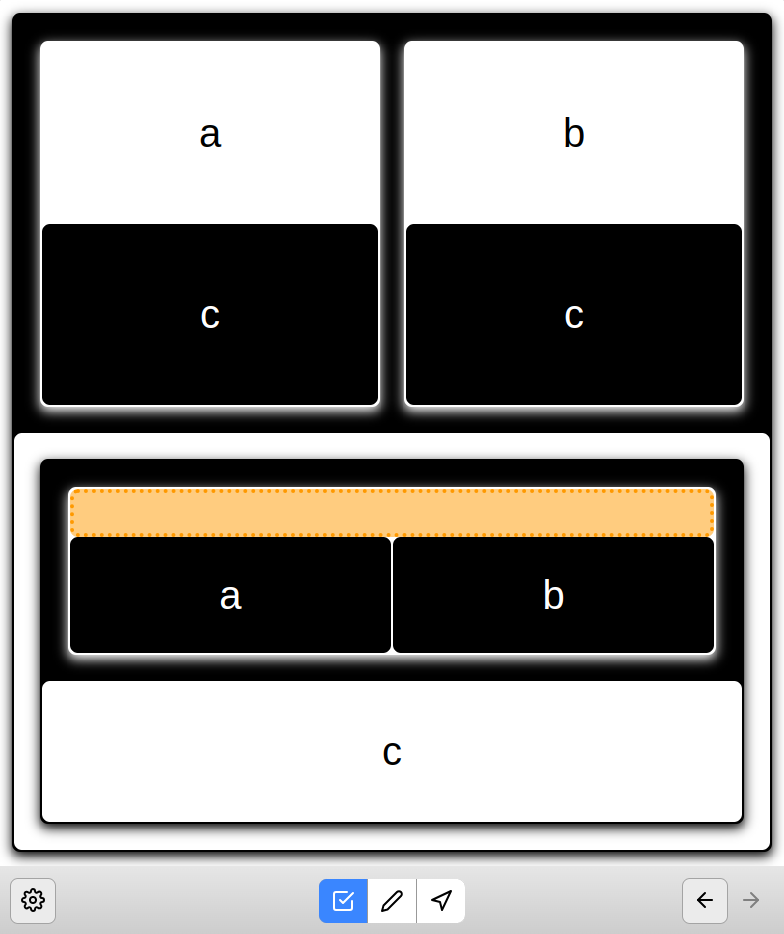
\includegraphics[width=0.7\textwidth]{flower-prover-proof-mode}
  \hspace{1em}
  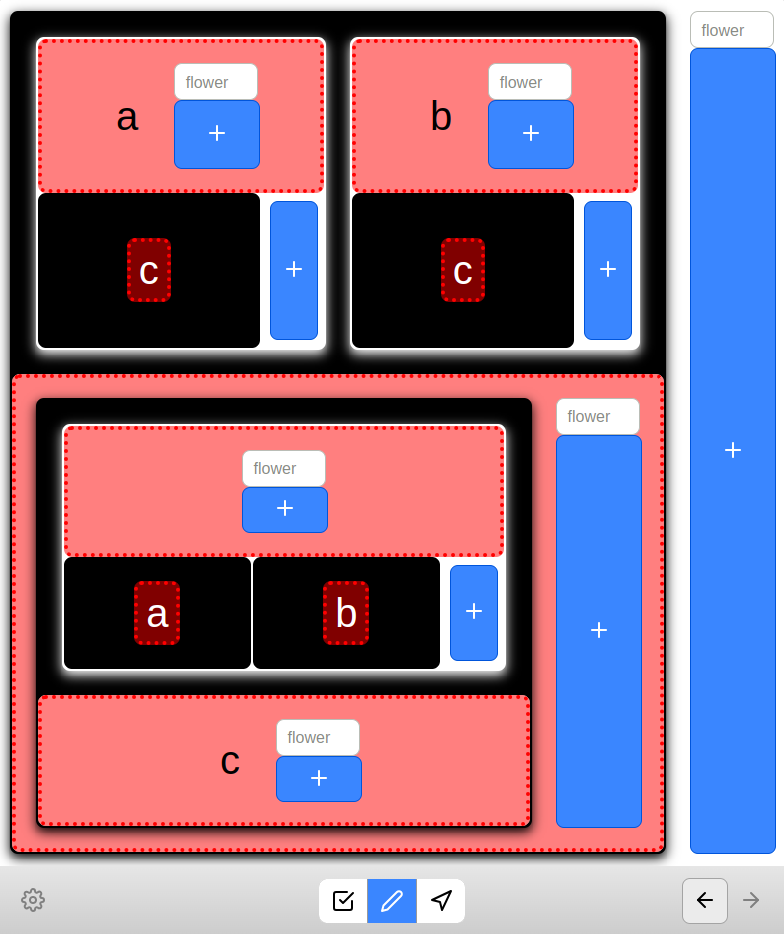
\includegraphics[width=0.7\textwidth]{flower-prover-edit-mode}
  \caption{\kl{Proof} mode (left) and \kl{Edit} mode (right) of the \kl{Flower\,\,Prover}}
  \labfig{flowers-prover-modes}
\end{figure*}

\reffig{flowers-prover-modes} shows side-by-side the same \kl{goal} representing the
flower $\flower{(\flower{a}{c}),(\flower{b}{c})}{(\flower{(\flower{}{a \sep
b})}{c})}$, but viewed through the two different modes. At any point during a
proof, the user can switch between the two modes by clicking on the
corresponding button in the \emph{mode selection bar}, located at the bottom of
the screen: \kl{Proof} and \kl{Edit} modes are mapped respectively to the left button with
a checkmark icon, and the middle button with a pencil icon.

\AP
It is also possible to \intro{Undo}/\intro{Redo} any action, whichever mode it was done
in, by clicking on the arrow buttons located on the bottom-right corner of the
screen. This is implemented by a simple stack recording the entire state of the
application, that is updated every time the user performs an action, and
popped/pushed when the user clicks on the \kl{Undo}/\kl{Redo} buttons. Since the
application state includes the current interaction mode, undoing/redoing an
action will automatically switch to the mode in which the action was performed.

\paragraph{\kl{Proof} actions}

\begin{table*}[h]
  \def\arraystretch{1.5}


% \hspace{-8em}
\subfloat[\Proof actions\labtab{flowers-proof-actions}]{
% \hspace{-0.1\textwidth}
\begin{tabular}{|c|C{5em}|C{11em}|}
\hline
\textbf{Action} & \textbf{Gesture} & \textbf{$\Nature$-rule} \\ \hline
\intro{Justify} & Click on $a$ & $$\R[\kl{poll{\da}}]{\Xi\select{\phantom{a}}}{\Xi\select{a}}$$ \\ \hline
\intro{Import} & \kl{DnD} of $\phi$ into $\Xi\hole$ & $$\prftree[l][r]{\kl{poll{\ua}}}{$\phi$ non-atomic}{\Xi\select{\phi}}{\Xi\select{\phantom{\phi}}}$$ \\ \hline
\intro{QED} & Click on empty petal & $$\R[\kl{epet}]{}{\flower{\gamma}{\garden{}{} \sep \Delta}}$$ \\ \hline
\intro{EFQ} & Click on empty pistil &
$$
\R[\kl{srep}]
{\R[\kl{epet}]
{}
{\flower{\Phi}{\cdot}}}
{\flower{\Phi, (\flower{\garden{}{}}{})}{\Delta}}
$$
\\ \hline
\intro{Case} & Click on empty pistil & $$\prftree[l][r]{\kl{srep}}{$n \geq 2$}{\flower{\Phi}{\fset{i}{n}{\flower{\gamma_i}{\Delta}}}}{\flower{\Phi, (\flower{\garden{}{}}{\fset{i}{n}{\gamma_i}})}{\Delta}}$$ \\ \hline
\intro{Unlock} & Click on empty pistil & $$\R[\kl{epis{\da}}]{\flower{\Phi, \Psi}{\Delta}}{\flower{\Phi, (\flower{\garden{}{}}{\Psi})}{\Delta}}$$ \\ \hline
\end{tabular}
}
\subfloat[\Edit actions\labtab{flowers-edit-actions}]{
\begin{tabular}{|c|C{7em}|C{7em}|}
\hline
\textbf{Action} & \textbf{Gesture} & \textbf{$\Culture$-rule} \\ \hline
\intro{Grow} & \texttt{Add} button in \kl{positive} bouquet & $$\R[\kl{grow}]{\Xi^+\select{\flower{}{\garden{}{}}}}{\Xi^+\select{\phantom{\flower{}{\garden{}{}}}}}$$ \\ \hline
\intro{Glue} & \texttt{Add} button in \kl{negative} corolla & $$\R[\kl{glue}]{\Xi^-\select{\flower{\gamma}{\garden{}{} \sep \Delta}}}{\Xi^-\select{\flower{\gamma}{\Delta}}}$$ \\ \hline
\intro{Insert} & \texttt{Add} button in grown bouquet/corolla & \kl{grow}/\kl{glue} \\ \hline
\intro{Delete} & Click on grown flower/petal & \kl{grow}/\kl{glue} \\ \hline
\intro{Crop} & Click on \kl{negative} flower & $$\R[\kl{crop}]{\Xi^-\select{\phantom{\phi}}}{\Xi^-\select{\phi}}$$ \\ \hline
\intro{Pull} & Click on \kl{positive} petal & $$\R[\kl{pull}]{\Xi^+\select{\flower{\gamma}{\Delta}}}{\Xi^+\select{\flower{\gamma}{\delta \sep \Delta}}}$$ \\ \hline
\end{tabular}
}

  \caption{Graphical actions of the \kl{Flower\,\,Prover}}
  \labfig{flowers-actions}
\end{table*}

\begin{figure*}[h]
  \newcommand{\incl}[1]{\vcenter{\hbox{\includegraphics[width=0.4\textwidth]{#1}}}}
$$
\hspace{-3em}
\begin{array}{cccccc@{\vspace{1em}}}
&\incl{flowers-prover-anim-0}
&\xstep{\Action{Case}}
&\incl{flowers-prover-anim-1}
&\xstep{\Action{Unlock}}
&\incl{flowers-prover-anim-2}
\\
\xstep{\Action{Import}}
&\incl{flowers-prover-anim-3}
&\xstep{\Action{Import}}
&\incl{flowers-prover-anim-4}
&\xstep{\Action{Justify}}
&\incl{flowers-prover-anim-5}
\\
\xstep{\Action{Unlock}}
&\incl{flowers-prover-anim-6}
&\xstep{\Action{Justify}}
&\incl{flowers-prover-anim-7}
&\xstep{\Action{QED}}
&\incl{flowers-prover-anim-8}
\end{array}
$$
  \caption{A sequence of \kl{Proof} actions in the \kl{Flower\,\,Prover}}
  \labfig{flowers-prover-anim}
\end{figure*}

\reftab{flowers-proof-actions} shows the precise mapping of \kl{Proof} actions to
$\Nature$-rules, together with the associated gestures for triggering them; and
\reffig{flowers-prover-anim} shows a sequence of screenshots of the \kl{Flower\,\,Prover}, capturing the execution of a sequence of \kl{Proof} actions reducing the
\kl{subgoal} $\flower{(\flower{}{a \sep b})}{c}$ to $\flower{b}{c}$. A few
comments are in order:

\begin{description}
  \item[Pollination] The most central actions are those implementing
  the \kl{pollination} rules \kl{poll{\da}} and \kl{poll{\ua}}, called respectively
  \kl{Justify} and \kl{Import}. In fact, they are \emph{less} general
  than those rules: one can only \kl{Justify} flowers that are \emph{atomic}
  by clicking on them, and \kl{Import} \emph{non-atomic} flowers by dragging
  and dropping them at the desired location. We conjecture that these
  restrictions do not jeopardize the completeness of $\Nature$-rules, and
  correspond to the process of $\eta$-expansion in \kl{$\lambda$-calculus}.
  
  \item[Suggestions]
  
  The fourth screenshot in \reffig{flowers-prover-anim} shows the flower $\phi
  \deq \flower{a}{c}$ being dragged in the process of an \kl{Import} action.
  If you look closely, you will notice that there are many areas whose border is
  highlighted with dashed yellow lines: these correspond to all \kl{contexts}
  $\Xi\hole$ where $\phi$ can be imported, i.e. such that
  $\chyp{\phi}{\Xi\hole}$. This is a first form of \emph{suggestion} in the
  \kl{Flower\,\,Prover}, indicating available valid actions to the user through visual
  feedback\sidenote{A similar mechanism is implemented in \kl{Actema}, where subterms
  that are possible drop targets for \kl{DnD} actions are also highlighted (see
  \refsec{validity}).}.

  In fact, every \kl{Proof} action has an associated visual cue, guiding interactive
  proof search by suggesting to the user areas of the \kl{goal} where she might want
  to focus her attention. Since every action other than \kl{Import} is
  performed by a \emph{click} gesture, the area that is highlighted corresponds
  precisely to the area that can be clicked for triggering the action: either a
  green box enclosing the justifiable atom for \kl{Justify} actions, an
  orange box covering the empty \kl{pistil} for \kl{EFQ}, \kl{Case} and
  \kl{Unlock} actions, or a green box covering the empty \kl{petal} for
  \kl{QED} actions.
  
  \itemAP[Fencing] We have already mentioned that we suspect that the
  \kl{epis} rule might be \kl{admissible}. However if it is not, one needs a
  corresponding graphical action in \kl{Proof} mode. While it is currently not
  implemented, we plan to add a \emph{selection} mechanism that allows the user
  to select a set of flowers in the \kl{goal}. Then, we could add a \intro{Fence}
  action, whose effect is to enclose the selected flowers in a \kl{petal} attached to
  an empty \kl{pistil}. This action could be mapped to a dedicated button in the
  toolbar that is visible only in \kl{Proof} mode, and enabled only when the
  selected flowers are juxtaposed in the same garden.
\end{description}

Since every \kl{Proof} action implements a $\Nature$-rule, it is guaranteed to be
\emph{\kl{invertible}}: the user never needs to \kl{Undo} a \kl{Proof} action in order to
complete a proof, because it always preserves the provability of the \kl{goal}. Of
course it might still be desirable to do so in specific cases, such as
\kl{Import} actions that may create unneeded copies of flowers\sidenote{In
this specific case, one might want to relax the atomic restriction on
\kl{Justify} actions, in order to avoid the recourse to \kl{Undo}
actions, which can only be performed at the top of the history stack.}.

\paragraph{\kl{Edit} actions}

\reftab{flowers-edit-actions} shows the precise mapping of \kl{Edit} actions to
$\Culture$-rules, together with the associated gestures for triggering them.
Like the edit mode of \texttt{vim}, \kl{Edit} actions are used to \emph{insert} and
\emph{delete} arbitrary flowers in the \kl{goal}:
\begin{description}
  \item[Insertion] The main interface mechanism that is currently
  implemented is the \texttt{Add} button: since the \kl{grow} rule allows to
  insert any flower in a \kl{positive} \kl{bouquet} (i.e. add a new \kl{subgoal}, just like the
  \kl(rule){cut} rule in \kl{sequent calculus}), we expose buttons in all the corresponding
  areas (blue ``+'' buttons in \reffig{flowers-prover-modes}), that can be
  clicked to insert a new flower precisely at the location of the button. There
  are two usage scenarios:
  \begin{itemize}
    \item if the user wants to insert an atomic flower, she can enter the name
    of the atom in a text field placed above the button. Clicking on the button
    will then insert an \kl{occurrence} of this atom;
    \item if the user wants to insert a non-atomic flower, she can leave the
    text field empty. Clicking on the button will then insert an empty flower
    with a single \kl{petal}.
  \end{itemize}
  In both cases, the inserted flower is marked internally by the system with a
  \texttt{grown} tag: this means that as long as the user does not leave
  \kl{Edit} mode, she can perform arbitrary insertions and deletions inside of
  the \texttt{grown} flower, disregarding any \kl{polarity} constraint normally
  imposed by $\Culture$-rules.
  
  Dually, the \kl{glue} rule is implemented by exposing \texttt{Add} buttons in
  all \kl{negative} \kl{corollas}: those have the effect of growing a new empty \kl{petal},
  that can be further edited through arbitrary insertions and deletions.

  \texttt{Grown} flowers/\kl{petals} are distinguished visually by having their
  border painted in blue. Leaving \kl{Edit} mode then has the effect of
  \emph{committing} every \kl{Edit} action, i.e. removing every \texttt{grown}
  tag in the entire \kl{goal}. This mechanism enables an incremental,
  step-by-step construction of flowers, that is still sound logically with
  respect to $\Culture$-rules.

  \item[Deletion] Deleting flowers and \kl{petals} is a more straightforward
  process: one just has to click on the corresponding area, which is highlighted
  in red. To avoid overlap, the area of a flower is identified with its
  \kl{pistil}. Thus areas subject to deletion are \kl{negative} atoms and
  flowers (\kl{crop} rule), \kl{positive} \kl{petals} (\kl{pull} rule), as well
  as any area marked as \texttt{grown}.
\end{description}

Since every \kl{Edit} action implements a $\Culture$-rule, it is guaranteed to be
\emph{non-\kl{invertible}}: the user might need to \kl{Undo} an \kl{Edit} action in order to
complete a proof, because it may break the provability of the \kl{goal}.

\paragraph{\intro{Navigation} mode}

The reader might have noticed that there is a third button with a navigation
icon on the right of the mode selection bar. It can be used to enter
\kl{Navigation} mode, the last mode of interaction that we intend to implement
in the future. The idea is that on real-life \kl{goals}, both the size and level
of nesting of flowers will quickly render the interface unusable, both for
reading/understanding the content and structure of \kl{goals}, and manipulating
them through pointing.

The purpose of the \kl{Navigation} mode is then to enable the user to
\emph{focus} on a specific \kl{subgoal}, by simply clicking on the corresponding
nested flower. This would make the \kl{subgoal} take up the whole screen, hiding
the outer context from view. Dually, it should also be possible to unfocus a
previously focused subgoal --- e.g. by clicking again on it --- so that the full
tree structure of the goal can be freely navigated. \kl{Proof-theoretically},
the \kl{Navigation} mode implements the \emph{functoriality} of rules, i.e. the
fact that they can be applied in \kl{contexts} of \emph{arbitrary} \kl{depth}.

\begin{remark}
This way of navigating tree structures represented as nested areas is typical of
\kl{zoomable user interfaces}, a strand of \kl{GUI} that has been developed by
many pioneers in the field of human-computer interaction such as Ivan Sutherland
in his \intro{Sketchpad} system \sidecite{10.1145/800265.810742}, and Alan Kay
in his \intro{Smalltalk} system \sidecite[4em]{goldberg_smalltalk-72_1976}.
\end{remark}

\paragraph{Automation}

The last feature of the \kl{Flower\,\,Prover} that we have implemented is the
\intro{Auto} \kl{Proof} action. It is similar in purpose to the \texttt{auto}
tactic of \kl{Coq}, that tries to simplify the \kl{goal} by performing a limited
(but customizable) amount of automation. The \kl{Auto} action is mapped to a
dedicated button in the bottom-left corner of the screen, which is only enabled
in \kl{Proof} mode (see \reffig{flowers-prover-modes}).

The idea is quite simple: since all click actions available to the user are
pre-computed by highlighting the corresponding areas, there can only be a finite
number of them. So why not try to apply them all automatically? Applying a click
action might generate new ones in the resulting \kl{goal}, so we have to perform
this until a fixpoint is reached. This is very much like the \kl[reproduction
phase]{reproduction} and \kl[decomposition phase]{decomposition} phases from the
\refproc{life} procedure of \refsec{flowers-search}, except that we also apply
the \kl{poll{\da}} rule (\kl{Justify} actions) wherever possible. The only
\kl{Proof} action that is not considered is the only \kl{DnD} action,
\kl{Import}. This is not surprising, since it corresponds to the \kl{poll{\ua}}
rule, which is the main source of complexity in the \kl{pollination phase} of
the \refproc{life} procedure, because of its ability to duplicate flowers of
arbitrary size.

In fact, one could fine-tune the level of automation by considering only a
\emph{subset} of all types of click actions. This is already what we do by
default, by leaving the application of \kl{Case} actions to the user. This is
motivated by the fact that the latter can induce an explosion in the size of the
\kl{goal}. One could even leave the configuration of automated action types to
the user with a dedicated interface. This could include an additional option for
executing \kl{Auto} systematically after every (other) \kl{Proof} action,
removing the need to click on the \kl{Auto} button. In this setting, any proof
in the \kl{Flower\,\,Prover} could be reduced to a sequence of \kl{Import} and
\kl{Case} actions.


\subsection{Towards a unified workflow}\labsubsec{flowers-unified}

\paragraph{Theories and goals}

In the \kl{proof view} of modern \kl{proof assistants} like \kl{Coq} and
\kl{Lean}, there is no distinction between local and global
\kl(sequent){contexts}: a \kl{subgoal} will inherit automatically every
hypothesis from its parent \kl{subgoals}, which are flattened into a big
unstructured list. To recreate this distinction and reduce the size of
\kl{goals} to a manageable level, the only interface mechanism offered to the
user is to exit interactive proof mode, and outsource chunks of the local
\kl(sequent){context} as additional global lemmas and definitions in the current
theory file.

Thus the user has to juggle between two different interfaces that manipulate two
distinct data structures: a traditional text editor for modifying
\emph{theories}, and an \kl{IDE} for writing and executing \kl{proof scripts}
that modify \emph{\kl{goals}}, themselves visualized in a separate \kl{proof
view}. This results in a duplication of means to achieve essentially the same
things: for instance, reordering two lemmas will require to cut and paste one of
them in the theory file, while reordering two hypotheses will require the use of
a dedicated \texttt{move} \kl{tactic}. Other examples can be found for renaming
definitions, applying lemmas, constructing functions, etc. Crucially, the two
interfaces cannot communicate straightforwardly with eachother. In fact,
communication is completely one-way: the user can only invoke definitions and
lemmas of the theory from her \kl{proof script}, by referring to their names.

The \kl{Flower\,\,Prover} can theoretically solve this divide, because it works on a
single data structure: flowers represent \emph{at the same time} the current
goal to be proved in \kl{Proof} mode, and the theories that are being built in \kl{Edit}
mode. Thus there are still two distinct modes/interfaces, but they work in
unison on the same data. The only (major) current limitation, is that we do not
have any way to \emph{save} proved lemmas for later reuse, because proving a
flower amounts to \emph{erasing} it from the current \kl{goal}. In a sense, theories
built in \kl{Edit} mode are only \emph{transient}: they live in \emph{working}
memory, and are disposed of as soon as they become justified in \kl{Proof} mode;
while we would like them to be \emph{persistent}, recorded in \emph{long-term}
memory along with their justifications (which would stay hidden from the user by
default). We will discuss in \refsec{Conclusion} some research directions that
we envision to achieve the latter. 

\paragraph{Statements and proofs}

Our above example of ``redundant'' manipulations targets \kl{imperative} tactic
languages, but the argument equally applies to more \kl{declarative} languages
like \kl{Isar}: the point is that the \emph{proof} language, be it
\kl{imperative} or \kl{declarative}, is separated both conceptually and through
its available means of interaction from the language of \emph{statements} used
to build theories. And this separation between proofs and statements is a
natural one that is hard to question, since it is rooted in what is arguably the
most important inspiration of formal logic, and also the form in which informal
mathematics present themselves: \emph{natural language}. Indeed, \kl{symbolic}
formulas reproduce the grammatical structure of sentences expressing logical
propositions, and formal proofs reproduce the inferential structure of arguments
built from sequences of sentences.

\paragraph{Context navigation}

After this little conceptual \textit{aparté}, let us come back to the problem of
managing contexts in proofs. In the \kl{Flower\,\,Prover}, the \emph{local}
context is naturally represented as \emph{everything that is displayed
on-screen}. This includes hypotheses that are available from \kl{pistils} at
various levels, but also potentially alternative \kl{goals} (adjacent
\kl{petals}) and further \kl{subgoals} (\kl{positively} nested flowers). Then
rather than being segregated in a separate interface (the text buffer of the
theory), the \emph{global} context is simply the \emph{entire} \kl{goal}. In
fact, there is no reason anymore to make a terminological distinction between
\kl{goals} and theories: a \kl{goal} is just a theory that has yet to be
justified, which can itself be identified with a partial proof (or a ``\kl{proof
term} with holes'' in \kl{type-theoretical} parlance)\sidenote{We will come back
to this idea of merging proofs and statements in the same data structure in the
conclusion, when discussing \emph{development calculi} and the \kl{Curry-Howard
correspondence}. Note however that it is already at work in \emph{dependent}
\kl{type theory}, where \kl{proof terms} can freely occur inside types. This is
exemplified in the \kl{Agda} \kl{proof assistant}, where all manipulations are
done directly on the partial proof/program text.}.

It would still be useful to be able to aggregate automatically the set of all
lemmas, definitions and hypotheses available in a focused subgoal located in
$\Phi\hole$, so that the user does not need to navigate up and down the
goal/proof tree all the time. This can be done with the help of the
\kl{pollination} relation (\refdef{pollination}), by defining the set of
\emph{available} flowers of $\Phi\hole$ as the the union
$\intro*\ctxt{\Phi\hole} \defeq \compr{\phi}{\chyp{\phi}{\Phi\hole}}$.

In terms of UI, we could then add a so-called \emph{shelf} that displays
$\ctxt{\Phi\hole}$ in all interaction modes. We anticipate only two kinds of
interaction with any flower $\phi \in \ctxt{\Phi\hole}$ in the shelf:
\begin{description}
  \item[Pollination (in \kl{Proof} mode)] the user can perform an
  \kl{Import} action by dragging $\phi$;
  \item[Jump to definition (in \kl{Navigation} mode)] the user can focus on
  the \kl{subgoal} where $\phi$ originates by clicking on $\phi$.
\end{description}

Since the shelf might contain \emph{a lot} of hypotheses, it will be important
to provide efficient ways to \emph{filter} or \emph{search} through its content.
We imagine three main ways of doing so\sidenote{The first two types of filtering
are already available in most \kl{proof assistants}, e.g. the \texttt{Search} command
of \kl{Coq}.}:
\begin{description}
  \item[By name] the user can type the \emph{name} of a hypothesis in a
  search bar. This implies that flowers have the ability to be named by the
  user.
  \item[By structure] the user can specify a \emph{pattern} that must
  be satisfied by all hypotheses in the shelf. A pattern is just a flower that
  contains pattern variables, which can match any flower. Thus patterns might be
  built with the same tools offered in \kl{Edit} mode.
  \item[By selection] the user can select subterms of the \kl{goal}, and then
  ask the system to display only hypotheses that can \emph{interact} with these
  subterms\sidenote{Here we imagine something along the lines of what we did for
  \kl{Actema} (see \refsec{funcs}).}.
\end{description}


\section{Conclusion}\labsec{Conclusion}

\subsection{Related works}

\paragraph{Intuitionistic EGs}
 
\begin{marginfigure}
  \begin{mathpar}
    \R[\intro{iter}]
      {\flower{\gamma}{\delta \sep \Delta}}
      {\flower{\gamma}{\delta \sep \delta \sep \Delta}}
    \and
    \R[\intro{deit}]
      {\flower{\gamma}{\delta \sep \delta \sep \Delta}}
      {\flower{\gamma}{\delta \sep \Delta}}
  \end{mathpar}
  \caption{(De)iteration rules for \kl{petals}}
  \labfig{flowers-deit-petals}
\end{marginfigure}

In the original \kl{IEGs} system of Oostra introduced in
\sidecite{oostra_graficos_2010}, the \kl{srep} rule is replaced by an extended
(de)iteration rule, that allows to duplicate/merge not only identical flowers,
but also identical \emph{\kl{petals}}, under the condition that they are
attached to the same \kl{pistil}\sidenote{``Cualquier lazo puede iterarse
adherido \emph{al mismo corte}'' \cite[p.~46]{oostra_graficos_2010}.} (rules
\kl{iter} and \kl{deit} in \reffig{flowers-deit-petals}). Thus in a sense,
(de)iteration on \kl{petals} is not as \emph{deep} as on whole flowers, where
the two identical flowers can be separated by an arbitrary number of layers;
which might seem like an arbitrary restriction. A posteriori, we rationalize
this choice by seeing it as an attempt to stay close to the original system
\kl{Alpha} of Peirce. In particular, (de)iteration on \kl{petals} is compatible
with the quest for \emph{\kl{illative atomicity}}, where all rules should be
expressed in terms of insertions and omissions (\refsec{atomicity}); while the
\kl{srep} rule is not. In our case, this is justified by our quest for an
\emph{\kl{invertible}} calculus (\kl{natural} fragment): indeed to simulate
\kl{srep} with \kl{petal} (de)iteration, one also needs the non-\kl{invertible}
$\Culture$-rule \kl{crop} (as well as the rule \kl{epis{\da}} of
\reffig{flowers-episda}), as illustrated by the \kl{srep}-free proof of
\reffig{flowers-srep-free}.

\begin{figure}
  \begin{mathpar}
  \prftree[r][d]{\rsf{poll{\ua}}}
  {\prftree[r][d]{\rsf{poll{\da}}}
  {\prftree[r][d]{\rsf{crop}}
  {\prftree[r]{\rsf{iter}}
  {\prftree[r][d]{\rsf{epis{\da}}}
  {\prftree[r]{\rsf{poll{\da}}}
  {\prftree[r]{\rsf{epet}}
  {}
  {\flower{(\flower{a}{c}),(\flower{b}{c}),c}{\garden{}{}}}}
  {\flower{(\flower{a}{c}),(\flower{b}{c}),c}{c}}}
  {\flower{(\flower{a}{c}),(\flower{b}{c}),(\flower{}{(\flower{}{c})})}{c}}}
  {\flower{(\flower{a}{c}),(\flower{b}{c}),(\flower{}{(\flower{}{c}) \sep (\flower{}{c})})}{c}}}
  {\flower{(\flower{a}{c}),(\flower{b}{c}),(\flower{}{(\flower{}{c}), a \sep (\flower{}{c}), b})}{c}}}
  {\flower{(\flower{a}{c}),(\flower{b}{c}),(\flower{}{(\flower{a}{c}), a \sep (\flower{b}{c}), b})}{c}}}
  {\flower{(\flower{a}{c}),(\flower{b}{c}),(\flower{}{a \sep b})}{c}}
\end{mathpar}
% \begin{mathpar}
%   \prftree[r][d]{\rsf{poll{\ua}}}
%   {\prftree[r][d]{\rsf{poll{\da}}}
%   {\prftree[r][d]{\rsf{crop}}
%   {\prftree[r]{\rsf{iter}}
%   {\prftree[r][d]{\rsf{srep}}
%   {\prftree[r]{\rsf{poll{\da}}}
%   {\prftree[r][d]{\rsf{epet}}
%   {}
%   {\flower{(\flower{a}{c}),(\flower{b}{c})}{(\flower{}{(\flower{c}{\garden{}{}})})}}}
%   {\flower{(\flower{a}{c}),(\flower{b}{c})}{(\flower{}{(\flower{c}{c})})}}}
%   {\flower{(\flower{a}{c}),(\flower{b}{c}),(\flower{}{(\flower{}{c})})}{c}}}
%   {\flower{(\flower{a}{c}),(\flower{b}{c}),(\flower{}{(\flower{}{c}) \sep (\flower{}{c})})}{c}}}
%   {\flower{(\flower{a}{c}),(\flower{b}{c}),(\flower{}{(\flower{}{c}), a \sep (\flower{}{c}), b})}{c}}}
%   {\flower{(\flower{a}{c}),(\flower{b}{c}),(\flower{}{(\flower{a}{c}), a \sep (\flower{b}{c}), b})}{c}}}
%   {\flower{(\flower{a}{c}),(\flower{b}{c}),(\flower{}{a \sep b})}{c}}
% \end{mathpar}
  \caption{Simulating the \kl{srep} rule by iterating \kl{petals}}
  \labfig{flowers-srep-free}
\end{figure}

In addition to his seminal work in \cite{oostra_graficos_2011}, Oostra describes
in \sidecite{oostra_graficos_2011} a natural extension of intuitionistic
\kl{Alpha} with \kl{LoIs}, in order to get an intuitionistic version of
\kl{Beta}. He also gives in \cite{10.1007/978-3-030-86062-2_16} formal soundness
and completeness proofs for intuitionistic \kl{Alpha}, based on a linear
notation for \kl{graphs}.

Ma and Pietarinen have developed in \cite{minghui_graphical_2019} their own
system of intuitionistic \kl{EGs} for propositional logic, with a different set
of inference rules than Oostra's. They give a more systematic proof theory,
including deduction, soundness and completeness theorems with respect to Heyting
algebras.

Our work brings several new contributions on top of those:
\begin{description}
  \item[Variadicity] Our multiset-based definition of flowers captures
  faithfully the \emph{variadic} nature of \kl{juxtaposition} and $n$-ary
  \kl{scrolls} in the diagrammatic syntax. In contrast, previous formalizations
  rely on a restricted inductive syntax which only captures \kl{graphs} that are
  isomorphic to formulas built with binary connectives\sidenote{Thus we reject
  the claim made in \cite{minghui_graphical_2019} that their system is ``solving
  the problem of defining a sequent calculus in the style of deep inference for
  intuitionistic propositional logic''. In our opinion, \kl{flowers} are closer
  to a form of nested sequent, although there is no consensus in the literature
  on what makes some inductive data structure a nested sequent.}.

  \item[Intuitionistic binders] While replacing \kl{LoIs} with \kl{binders}
  and variables has already been done by Sowa in the context of classical \kl{EGs}
  \cite{sowa_peirces_2011}, it seems like we are the first to adapt the idea to
  the intuitionistic setting.

  \item[Analyticity] To our knowledge, we are the first to give a Kripke
  semantics to a syntax based on \kl{EGs}, and to use this to obtain an
  \kl{analyticity} result, as discussed in \refsec{Completeness}.  

  \item[Invertibility] The \kl{natural} fragment of the flower calculus appears
  to be the first proof system based on \kl{EGs} where all rules are
  \emph{invertible}.
\end{description}

\paragraph{Focusing}

There is a formal connection between the \kl{poll{\ua}} rule of the \kl{flower
calculus}, and the \emph{absorption} rule $[\mathbf{A}]$ of the dyadic system
$\Sigma_2$ of Andreoli, that handles the \kl{focusing} behavior of exponentials in
linear logic \sidecite{andreoli1992}. Indeed, both rules duplicate a formula
available in the (non-linear) \kl{context} of the sequent/location where the rule is
applied, in order to enable further usage of the formula at said location. While
the absorption rule removes the need for permutation-equivalences between proofs
involving the \emph{\kl{contraction}} rule, the identity rule $[I]$ of $\Sigma_2$
removes the need for the \emph{\kl{weakening}} rule by discarding the non-linear
\kl{context} in one go, just as the \kl{epet} rule of the \kl{flower calculus} renders
the \kl{crop} rule \kl{admissible}.

Sonia Marin has noticed the connection between \emph{bipoles} in \kl{focused}
proofs, and the class of geometric/\kl{coherent formulas}, where the former are seen
as a generalization of the latter \sidecite{marin_axioms_2022}. This is to be
related to our own identification of \kl{$n$-ary scrolls}/flowers as a recursive
generalization of \kl{coherent formulas} at the end of \refsec{IEGs}.

Two years earlier, Brock-Nannestad and Ilik had already made some implicit
connections between \kl{focused} proofs and \kl{coherent formulas}, through their
\emph{exponential normal form} for \kl{intuitionistic} formulas based on Tarski's
highschool identities \sidecite{brock-nannestad_intuitionistic_2019}. Quite
remarkably, \kl{first-order} formulas in their exponential normal form have the exact
same structure as flowers
\cite[Definition~4.2]{brock-nannestad_intuitionistic_2019}. However, the \kl{sequent
calculus} \intro{HS} based on them makes the tradeoff opposite to that of the
natural fragment $\Nature$ of the \kl{flower calculus}: every \kl{inference rule} is
\emph{non}-\kl{invertible}, but the calculus is \kl{contraction}-free. One advantage of
this tradeoff is that they can easily show termination of proof search, while we
have not found a terminating procedure yet for the \kl{flower calculus}. The authors
also mention that \kl{HS} could be turned into a \kl{deep inference} calculus in the
style of \kl{G4ip}\sidenote{This is just another name for the system \kl{LJT}
of Dyckhoff already mentioned in \refch{bubbles-symm}.}.

\paragraph{Development calculi}

In \refsec{flowers-prover}, we have seen how the rules of the \kl{flower
calculus} can be understood as a set of (graphical) \kl{tactics} for building
partial proofs interactively. In Chapter 3 of his thesis
\sidecite{ayers_thesis}, Ayers calls such systems \emph{development calculi}. In
particular, he presents his own development calculus inspired by McBride's OLEGs
system \sidecite{mcbride_dependently_2000} and G\&G's prover
\sidecite{ganesalingam_fully_2017} called the \texttt{Box} calculus, where both
goals and partial proofs are represented by the same \texttt{Box} data
structure. Once again, \texttt{Box}es seem to share a very similar structure
with flowers, which was here motivated by the need to avoid backtracking by
having the ability to maintain a disjunction of \kl{goals} with so-called
\emph{disjunctive pairs}, corresponding to the \kl{petals} of flowers. The main
difference is that the \texttt{Box} calculus is based on dependent \kl{type
theory} instead of \kl{first-order logic}: this allows to store the partial
\kl{proof terms} inside of the \texttt{Box}es themselves, while this information
is lost during the construction of flowers (but might be reconstructed from the
sequence of graphical actions and the initial \kl{goal}).

Ayers also mentions the category-theoretical treatment of development calculi by
Sterling and Harper \sidecite{sterling_algebraic_2017}, that abstracts from any
particular type of \kl{judgment}. Thus it might be possible to fit the \kl{flower
calculus} into this framework, by identifying the set of flowers $\flowers$ as a
category of \emph{nested \kl{judgments}}\sidenote{Nested \kl{judgments} are already
considered in some recent categorical semantics of \kl{type theory}, and in
particular those in Sterling's thesis \cite{Sterling2022}. See also
\cite{huang2023synthetic} for a (technical) introduction to the subject.}.

\paragraph{Subformula linking}

Our notion of \emph{\kl{vehicle}} (\refdef{vehicle}) takes its terminology from
Girard, who started giving this name to the set of axiom links of a proof
structure in his transcendental syntax\sidenote{Also, it conveys nicely the idea
that the \kl{vehicle} is the fundamental structure that \emph{drives} the proof
search algorithm.} \sidecite{girard_2017}. But the idea of connecting dual
\kl{occurrences} of atoms, and thus forming a graph with an associated adjacency
matrix whose structure can be exploited in proof search, really dates back to
the \emph{connection method} developed independently by Bibel and Andrews in the
1970s \sidecite{Bibel:2009}. Otten and Kreitz have adapted the connection method
to \kl{intuitionistic} logic \sidecite{10.1007/3-540-59338-1_32}, stating that it is
especially well-suited in an interactive theorem proving environment. Thus it
might be instructive to learn from their proof search algorithm to fix ours.

In fact all proof search procedures designed in this thesis, whether for \kl{bubble
calculi} (\refsubsec{bubbles-search}) or the \kl{flower calculus}
(\refsec{flowers-search}), rest on the fundamental observation coming from the
\kl{subformula linking} methodology of Chaudhuri \sidecite{Chaudhuri2013}, that the
construction of proofs in \kl{deep inference} systems can be driven efficiently and
incrementally by the connection of dual atoms. With its \kl{pollination} rules, the
\kl{flower calculus} allows for a particularly elegant implementation of \kl{subformula
linking} that abstracts away from the syntactic bureaucracy of \kl{symbolic}
connectives, as witnessed by the \kl{pollination phase} of our search procedure. In
\refsubsec{bubbles-search}, we sketched some ideas that blur the frontier
between automated and interactive proof search, notably with the so-called
\emph{rule of thumb} which is another manifestation of \kl{subformula linking}. This
integration of automated and interactive aspects is also at work in the \kl{Flower\,\,Prover}, and it would be interesting to investigate further how to incorporate
our drag-and-drop proof \kl{tactic} (\refch{pba}), but also other \kl{symbolic}
manipulation techniques introduced in the first part of this thesis, into the
\kl{iconic} framework of the \kl{Flower\,\,Prover}.

\paragraph{Analyticity}

We have not discussed the rationale behind our notion of \kl{analyticity}, be it
historical or formal arguments explaining its origins, motivations and
consequences. In a recent article \sidecite{bruscoli_analyticity_2019}, Bruscoli
and Guglielmi propose such a detailed discussion around a precise and generic
definition of \kl{analyticity} for \kl{deep inference} \kl{proof systems} (especially
the \kl{calculus of structures}), which at a glance seems to encompass our own
definition. It would be interesting to study more deeply their work, and related
parts of the \kl{deep inference} literature concerned with \kl{analyticity} and its
applications to efficient proof search procedures
\sidecite{kahramanogullari_reducing_2006,lmcs:1089,10.1145/2003476.2003501,chaudhuri:hal-00772420,10.1007/978-3-662-49630-5_23}.

\subsection{Future works}

\paragraph{Metatheory}

In \refsec{Calculus}, we already mentioned the variant $\Nature \setminus
\{\kl{epis}\} \cup \{\kl{crep}\}$ of the natural fragment, that we conjecture
to enjoy both soundness, completeness and a deduction theorem. But these last
two results shall prove particularly harder to prove, and we currently have very
few insights into how to extend the proofs of this chapter to this setting.
Also, this is not withstanding the fact that we do not really see any practical
applications for such results as of yet. Our initial motivation was to show the
admissibility of the \kl{epis} rule, because it never appears in concrete
proofs. But if this requires adding the \kl{crep} rule instead, then it greatly
reduces the pratical interest of the whole endeavor, since the \kl{crep} rule
does not look particularly well-suited to either automated or interactive
theorem proving.

Another line of research would concern properties of \emph{locality}, in the
sense coined by the \kl{deep inference} community with systems like \kl{SKS} (see
\refsec{eg-completeness}). As mentioned in \refsec{flowers-prover}, we
conjecture that the \kl{poll{\da}} and \kl{poll{\ua}} rules can be restricted
respectively to atomic and non-atomic flowers. But this is less satisfying than
in the \kl{calculus of structures}, where one component of \kl{poll{\ua}}, the
duplicating \emph{\kl{contraction}} rule, can be restricted to atomic formulas. This
probably comes from the fact that \kl{poll{\ua}} also serves the purpose of
\emph{moving} flowers deeper, as witnessed by the \kl{DnD} \kl{Import} action of
the \kl{Flower\,\,Prover}: in the \kl{calculus of structures}, this role is fulfilled by
\emph{switch} rules, which cannot be restricted to atomic structures. The only
solution might be to \emph{simulate} a local \kl{calculus of structures} for
\kl{intuitionistic} logic, like the system \kl{ISp} of Tiu
\sidecite{tiu_local_2006}.

Lastly, it would be interesting to exhibit an \emph{internal}, syntactic
procedure for eliminating cultural $\Culture$-rules in proofs, just like Gentzen
showed \kl{cut-elimination} in \kl{sequent calculus}\sidenote{A sort of
\emph{cult}-elimination, so to speak.}. In this work we preferred a more
semantic approach, because it was simpler and at the right level of abstraction
for our needs. We might be able to take some inspiration from the
\kl{cut-elimination} proofs of \kl{calculi of structures}, which are indeed notoriously
involved.

\paragraph{Automated proof search}

We shall investigate the current sources of non-termination and incompleteness
for our \refproc{life} proof search procedure, through further testing on the
ILTP dataset. If we succeed in passing all tests, the natural continuation will
be to provide formal proofs of termination and completeness. A follow-up
direction would be to extend our algorithm to the \kl{first-order} setting by adding
heuristics for handling \kl{sprinklers}, thus losing completeness.

Another direction of research would consist in comparing our algorithm to
existing search procedures for \kl{EGs}, in particular one that was originally
developed by Peirce, and described by Oostra in \sidecite{oostra_advances_2022}.

\paragraph{Curry-Howard}

We have begun to sketch some ideas for a \kl{Curry-Howard correspondence}, where
flowers and \kl{Proof} actions for justifying them ($\Nature$-rules) are identified
respectively with \emph{normal} and \emph{neutral} \kl{terms} of the simply-typed
\kl{$\lambda$-calculus}. For instance, the computational counterpart of the rule
\kl{poll{\da}} in \kl{pistils} would be a kind of \emph{function application}
expressed by the following \kl{app} rule, which is highly reminiscent of the
instantiation rule \kl{ipis}:
$$
\R[\intro{app}]
  {\Xi\select{t~u : (\flower{\subst{\Phi}{u}{x}}{\subst{\Delta}{u}{x}})}}
  {\Xi\select{t : (\flower{\Phi, x : \phi}{\Delta})}}
$$
Given a flower $\phi$ and a neutral \kl{term} $t$, i.e. an $n$-ary function
application of the form $x~t_1 \ldots t_n$, the expression $t : \phi$ is a
\emph{\kl{term} annotation}, that should be read in context as ``this \kl{occurrence} of
$\phi$ is justified by $t$''. Interestingly, $\phi$ itself may contain \kl{term}
annotations, mimicking the fact that normal and neutral \kl{terms} can be defined by
mutual recursion. Then in the \kl{app} rule, we do not just erase the formula
$\phi$ as in the \kl{poll{\da}} rule, but also keep track of the flow of
information by appending the argument $u$ to the justification $t$ (where
$\chyp{(u : \phi)}{\Xi\hole}$), and substituting $u$ to every \kl{occurrence} of the
hypothetical justification $x$ of $\phi$ in $\Phi$ and $\Delta$.

As of now the syntax of annotated flowers is not yet stable, and it is unclear
what would be the computational interpretation of flowers with $n \not= 1$
\kl{petals}. In particular for disjunctive flowers ($n > 1$), it seems that we are
closer to a notion of non-deterministic or parallel computation, than to the
usual branching computation of sum or inductive \kl{types}.

If our intuition is right, then the fact that flowers correspond to (normal)
\kl{$\lambda$-terms} would embody syntactically a recent motto from Miquel stemming
from his study of the foundations of \kl{forcing} and realizability in
implicative
algebras, where ``elements can be seen both as truth values and as (generalized)
realizers, thus \textbf{blurring the frontier between proofs and
types}''\sidenote{Another recent, related incarnation of this phenomenon is the
correspondence uncovered by Haydon between a linear version of \kl{EGs} already
appearing in Peirce's writings, and the proof nets of Girard for linear logic
\cite{haydon_eg_pn}.} \sidecite{miquel_implicative_2020}. Or as he put it in a
recent talk \cite{miquel_implicative_topos_2022}, we get the ultimate
Curry-Howard identification:
$$
\text{\textbf{Realizer}} = \text{\textbf{Program}} = \text{\textbf{Formula}} = \text{\textbf{Type}}
$$
This could also form the basis for further studies on the connections between
\kl{EGs} and (dependent) \kl{type theory}, and ultimately lead to a tight
integration of the \kl{Flower\,\,Prover} with \kl{proof assistants} based on the
latter such as \kl{Coq}, \kl{Lean} and \kl{Agda}. Existing explorations of the
links between \kl{type theory} and \kl{deep inference} include, in historical
order:
\begin{itemize}
  \item a first attempt by Brünnler and McKinnley to devise a \kl{Curry-Howard
  correspondence} for a simple \kl{intuitionistic} \kl{deep inference} calculus with
  conjunction and implication \sidecite{cervesato_algorithmic_2008};
  \item the thesis of Nicolas Guenot, and more precisely the part on "Nested
  Proofs as Programs" where he gives a correspondence between simply-typed
  \kl{$\lambda$-calculi} with explicit substitutions at one end, and calculi of
  structures (Chapter 6) and \kl{nested sequent} calculi (Chapter 5) for the
  implicational fragment of \kl{intuitionistic} logic at the other end
  \cite{guenot_nested_2013};
  \item the atomic \kl{$\lambda$-calculus}, a simply-typed \kl{$\lambda$-calculus} with
  explicit sharing that has a \kl{Curry-Howard correspondence} with proofs in the
  formalism of \emph{open deduction} \sidecite{gundersen_atomic_2013};
  \item a \kl{type} system for interaction nets based on a \kl{calculus of structures} for
  Multiplicative Exponential Linear Logic \sidecite{gimenez_structure_2013};
  \item the thesis of Fanny He, that explores a \kl{classical} variant of the atomic
  \kl{$\lambda$-calculus} based on Saurin's $\Lambda\mu$-calculus
  \sidecite{he_fanny_thesis};
  \item the \emph{spinal} atomic \kl{$\lambda$-calculus}, an extension and
  improvement on the atomic \kl{$\lambda$-calculus} based on a computational
  interpretation of the \emph{switch} rule \sidecite{goubault-larrecq_spinal_2020};
  \item the \emph{collection calculus} that subsumes resource,
  intersection-typed and simply-typed \kl{$\lambda$-calculi}, with a \kl{type} system
  again in open deduction \sidecite{guerrieri_deep_2021};
  \item Ongoing research by Kaustuv Chaudhuri to extend \kl{subformula linking} to
  dependent \kl{type theory}\sidenote{Private communication.}.
\end{itemize}
The work of Guenot on computational interpretations of \kl{nested sequent} calculi
seems closest to the syntax of flowers. Indeed, \kl{nested sequents} are variadic by
nature, and his version of \kl{nested sequents} in particular exploits the
possibility to have \emph{negative} \kl{occurrences} of sequents. Combined with the
dependently-typed \texttt{Box}es of Ayers mentioned earlier (which cannot be
nested negatively), this should provide great insights for the powerful,
dependently-typed version of the \kl{flower calculus} that we seek for.

\paragraph{Flower Prover}

We have already described many features in \refsec{flowers-prover} that we
intend to implement in the future. This includes the \kl{Navigation} mode, the
ability to \emph{select} flowers, the \kl{Fence} \kl{Proof} action, and the
\emph{shelf} mechanism.

The next step would be to support \kl{first-order} reasoning by adding \kl{sprinklers} and
\kl{first-order} terms, and devising graphical actions for the rules $\{\kl{ipis},
\kl{ipet}\}$ in \kl{Proof} mode, and $\{\kl{apis}, \kl{apet}\}$ in \kl{Edit} mode.

Last but not least, we want to provide a way to \emph{save} proved lemmas along
with their proof, so that they can be reused and read statically. This will be
crucial for \emph{\kl{proof evolution}}\sidenote{See also
\refsubsec{proof-evolution}.}, and will probably rely on the computational,
dependently-typed version of the \kl{flower calculus} sketched above, where \kl{proof
terms} can appear inside flowers.

\subsection{Theory vs. Practice}

Finally, it should be noted that Peirce did not think of \kl{EGs} as a calculus that
could aid in performing reasoning \emph{per se}, but rather as a tool for
analyzing the finer structure of logical endeavor
\cite[pp.~110--111]{Roberts+1973}:
\begin{quote}
  [...] the purpose which the system was designed to fulfill was ``to enable us
to separate reasoning into its smallest steps so that each one may be examined
by itself'' (Ms 455, p.~2). The aim was not to facilitate reasoning, but to
facilitate the study of reasoning.
\end{quote}

The various achievements presented in this chapter incite us to depart from this
conception. Indeed, our particular viewpoint on the \kl{illative transformations},
that emphasizes \kl{goal}-reduction through \kl{invertible} and \kl{analytic}
rules, enabled us to design a novel and promising type of graphical interface
for interactive proof building, which integrates easily and elegantly some
(limited) forms of automation. This was also made possible by the use of
variables instead of \kl{lines of identity}, trading a heavy graphical apparatus
with local \kl{inference rules} for a simple, well-known textual syntax with
complex (but automated) global dynamics in the form of \kl{substitutions}. Hence
we believe the \emph{opposite}, that \kl{EGs} \emph{can} form the basis for an
ergonomic calculus of logical deduction, in addition to being a powerful tool
for meta-logical analysis.


\end{scope}
